\documentclass[10pt,twocolumn,a4paper]{article}
\usepackage[a4paper,top=18mm,bottom=19mm,left=15mm,right=15mm,columnsep=6mm]{geometry}
\usepackage{mathptmx}
\usepackage[T1]{fontenc}
\usepackage[utf8]{inputenc}
\usepackage{amsmath,amssymb}
\usepackage{graphicx}
\graphicspath{{../}{../figures/}{./}{figures/}}
\usepackage{booktabs}
\usepackage{tabularx}
\usepackage{array}
\usepackage{float}
\usepackage{xcolor}
\usepackage{fancyhdr}
\usepackage{microtype}
\usepackage{caption}
\usepackage[colorlinks=true,linkcolor=blue!65!black,citecolor=blue!65!black,urlcolor=blue!65!black,
            pdftitle={Comparative Evaluation of Machine Learning Classifiers for Extreme Rainfall at the Kathmandu Airport Grid Cell, Nepal},
            pdfauthor={Bishow Gurung (College ID: 260005, CUID: 17624457)},
            pdfsubject={STW7072CEM Machine Learning Coursework}]{hyperref}

\sloppy
\setlength{\emergencystretch}{3em}
\tolerance=2000
\hbadness=10000
\hfuzz=2pt

\renewcommand{\thesection}{\Roman{section}}
\renewcommand{\thesubsection}{\Alph{subsection}}
\renewcommand{\thesubsubsection}{\arabic{subsubsection}}
\renewcommand{\thetable}{\Roman{table}}

\captionsetup[figure]{
  font=footnotesize,
  labelfont=bf,
  name={Fig.},
  labelsep=period,
  justification=justified,
  singlelinecheck=false
}
\captionsetup[table]{
  font=footnotesize,
  labelfont=bf,
  name={TABLE},
  labelsep=newline,
  justification=centering
}

\makeatletter
\renewcommand{\@seccntformat}[1]{%
  \csname the#1format\endcsname
}
\newcommand{\thesectionformat}{\thesection.\quad}
\newcommand{\thesubsectionformat}{\thesubsection.\quad}
\newcommand{\thesubsubsectionformat}{\thesubsubsection)\quad}

\renewcommand{\section}{\@startsection{section}{1}{\z@}%
  {-10pt \@plus -2pt \@minus -1pt}%
  {4.5pt \@plus 1pt}%
  {\centering\normalfont\normalsize\bfseries\scshape}}
\renewcommand{\subsection}{\@startsection{subsection}{2}{\z@}%
  {-7pt \@plus -1.5pt \@minus -0.5pt}%
  {3pt \@plus 0.5pt}%
  {\normalfont\normalsize\bfseries\itshape}}
\renewcommand{\subsubsection}{\@startsection{subsubsection}{3}{0.5em}%
  {-5pt \@plus -1pt \@minus -0.5pt}%
  {2pt \@plus 0.5pt}%
  {\normalfont\normalsize\bfseries\itshape}}
\makeatother

\newcommand{\algheading}[1]{%
  \par\vspace{2.5pt}\noindent{\small\bfseries #1}\par\vspace{1pt}\noindent\ignorespaces
}

\pagestyle{fancy}
\fancyhf{}
\fancyhead{}
\fancyfoot[C]{\thepage}
\renewcommand{\headrulewidth}{0pt}
\renewcommand{\footrulewidth}{0pt}

\setlength{\parskip}{2pt plus 0.5pt minus 0.5pt}
\setlength{\textfloatsep}{6pt plus 2pt minus 2pt}
\setlength{\floatsep}{5pt plus 2pt minus 2pt}
\setlength{\intextsep}{5pt plus 2pt minus 2pt}

\begin{document}
\raggedbottom
\thispagestyle{fancy}

\twocolumn[{%
\begin{@twocolumnfalse}
\begin{center}
{\LARGE\bfseries Comparative Evaluation of Machine Learning Classifiers for Extreme Rainfall at the Kathmandu Airport Grid Cell, Nepal\par}
\vspace{8pt}
{\large\textbf{Bishow Gurung}\par}
\vspace{2pt}
{\normalsize College ID: 260005 $\mid$ Coventry University ID: 17624457\par}
{\normalsize\textit{MSc Data Science and Computational Intelligence}\par}
{\normalsize Softwarica College of IT \& E-Commerce, Kathmandu, Nepal\par}
{\small Email: \href{mailto:260005@softwarica.edu.np}{260005@softwarica.edu.np} $\mid$ Module: STW7072CEM Machine Learning\par}
\vspace{10pt}
\end{center}
\end{@twocolumnfalse}
}]

{\small\noindent{\bfseries\textit{Abstract}---}{\bfseries Severe monsoon downpours in the Kathmandu Valley regularly cause destructive flash floods, yet identifying these rare storms from gridded weather records remains challenging because dry and moderate days vastly outnumber extreme rainfall days. Guided by three consolidated research objectives, this study develops a leak-free daily weather dataset spanning {\normalfont 30} years ({\normalfont 1995}--{\normalfont 2024}, {\normalfont 10,958} raw days and {\normalfont 10,951} complete records after lag creation) for the Tribhuvan International Airport grid cell. Using a strict chronological split, historical records from {\normalfont 1995} to {\normalfont 2018} ({\normalfont 8,759} days, {\normalfont 439} extreme days above {\normalfont 13.74} mm/day) are used exclusively for model training, while records from {\normalfont 2019} to {\normalfont 2024} ({\normalfont 2,192} days, {\normalfont 164} extreme days) serve as an unseen holdout test set. First, Principal Component Analysis (PCA) compresses {\normalfont 22} weather predictors into {\normalfont 7} components retaining {\normalfont 91.46\%} of data variation, Fast Independent Component Analysis (FastICA) isolates sharp storm bursts, and K-Means clustering identifies three seasonal regimes in which a single wet monsoon cluster captures {\normalfont 94.99\%} ({\normalfont 417} of {\normalfont 439}) of training storms. Second, five supervised classifiers are compared: Logistic Regression, Decision Tree (CART), Radial Basis Function Support Vector Machine (RBF-SVM), Random Forest, and k-Nearest Neighbours (k-NN). On the {\normalfont 2019}--{\normalfont 2024} test set, Random Forest delivers the best overall balance between storm detection and false-alarm control (F{\normalfont 1}-score of {\normalfont 0.4385}, Precision-Recall AUC of {\normalfont 0.5517}, ROC-AUC of {\normalfont 0.9349}, and {\normalfont 90.24\%} recall), while class-weighted Logistic Regression achieves the highest storm sensitivity ({\normalfont 96.34\%} recall, catching {\normalfont 158} of {\normalfont 164} storms). In contrast, unweighted k-NN reaches {\normalfont 93.16\%} overall accuracy but misses {\normalfont 71.34\%} of extreme storms ({\normalfont 28.66\%} recall). Finally, lowering the Random Forest warning threshold to {\normalfont 0.30} based on training cross-validation under a {\normalfont 15}-to-{\normalfont 1} missed-flood penalty raises test recall to {\normalfont 98.17\%} ({\normalfont 161} of {\normalfont 164} storms detected) and successfully flags the catastrophic {\normalfont 24}--{\normalfont 28} September {\normalfont 2024} Kathmandu flood both on the same day and {\normalfont 24} hours in advance.}

\vspace{4pt}
\noindent{\bfseries\textit{Index Terms}---Cost-sensitive threshold tuning, extreme rainfall classification, imbalanced weather data, Kathmandu Valley, machine learning comparison, monsoon flood warning.\par}\par}

\section{Introduction}

\subsection{Background and Motivation}
Heavy monsoon downpours and late-season low-pressure storms frequently trigger flash flooding and infrastructure damage across central Nepal \cite{ref1,ref2,ref3}. Surrounded by mountain ridges rising above 2,500 metres, the bowl-shaped Kathmandu Valley (1,300--1,400 m elevation) channels runoff from the Bagmati and Bishnumati rivers through a single narrow outlet at the Chobhar gorge \cite{ref4,ref5}. Rapid urban growth has replaced open floodplains with concrete, meaning that daily rainfall above 14 to 25 mm/day quickly overwhelms drainage networks \cite{ref5,ref6,ref7,ref8}. During 24--28 September 2024, five consecutive days of extreme rain peaking at 93.26 mm/day at the Tribhuvan International Airport grid cell halted flights, flooded riverside settlements, and claimed over 240 lives, underscoring the urgent need for reliable statistical flood warning tools \cite{ref6,ref7}.

While physics-based weather models capture regional circulation \cite{ref9,ref10,ref11}, their coarse grid spacing smooths out local valley cloudbursts and requires heavy computing resources \cite{ref3,ref12}. Machine learning classifiers offer a practical alternative by mapping daily temperature, humidity, pressure, solar radiation, and past rainfall to storm probabilities \cite{ref1,ref2,ref12}. However, building a trustworthy classifier requires overcoming three challenges: (1) extreme rain above the 95th percentile (13.74 mm/day) occurs on only 5.01\% of training days, causing standard models to favour the dry majority class \cite{ref2,ref3}; (2) multi-day monsoon persistence causes data leakage under random splits \cite{ref1,ref13}; and (3) missing a damaging flood is far costlier than issuing a precautionary standby alert \cite{ref3,ref6}.

\subsection{Research Aim and Objectives}
The primary aim of this study is to compare supervised machine learning classifiers and unsupervised weather pattern analysis techniques for identifying extreme daily rainfall at the Kathmandu Airport grid cell, supporting reliable and cost-sensitive early flood warning. To achieve this aim, the study is structured around three consolidated Research Objectives (RO1--RO3):

\subsubsection{RO1 (Data Preparation and Unsupervised Meteorological Pattern Analysis)}
To develop a reproducible and leakage-free meteorological dataset for extreme rainfall classification at the Kathmandu Airport grid cell using NASA POWER/MERRA-2 historical observations (1995--2024), incorporating physically meaningful feature engineering, chronological data partitioning, and unsupervised techniques (PCA, FastICA, and K-Means clustering) to investigate underlying meteorological patterns and rainfall regimes.

\subsubsection{RO2 (Comparative Evaluation of Machine Learning Algorithms)}
To implement and critically compare five supervised machine learning classifiers---Logistic Regression, Decision Tree (CART), Radial Basis Function Support Vector Machine (RBF-SVM), Random Forest, and k-Nearest Neighbours (k-NN)---evaluating their effectiveness in identifying extreme rainfall events under severe class imbalance in terms of predictive performance, interpretability, probability calibration, and computational efficiency.

\subsubsection{RO3 (Operational Evaluation and Cost-Sensitive Extreme Rainfall Prediction)}
To evaluate the operational suitability and reliability of the developed classification framework through cost-sensitive threshold optimisation, strict 24-hour lead-time forecasting, wet-day extreme rainfall classification, and retrospective validation against the September 2024 Kathmandu flood event.

\section{Literature Review}

\subsection{Himalayan Extreme Rainfall Trends}
Multi-decade station studies confirm that extreme monsoon rain in the Kathmandu Valley is intensifying even as total rainy days fluctuate \cite{ref4,ref5,ref8}. Analysing station observations across the valley, Chaulagain \textit{et al.} \cite{ref4} and Khanal \textit{et al.} \cite{ref5} linked rising 95th-percentile downpours to large-scale moisture transport from the Bay of Bengal and rapid urban surface heating. Phuyal \cite{ref8} further showed that heavy downpours are strongly concentrated between June and September along the valley floor and surrounding hillslopes. Across the wider Himalayan region, Wani \textit{et al.} \cite{ref9}, Pujara and Paudel \cite{ref10}, and Bashyal \textit{et al.} \cite{ref11} demonstrated that traditional linear time-series models fail to capture sudden mountain cloudbursts, whereas complex deep neural networks require large computing budgets and dense local sensor networks \cite{ref11,ref12}, motivating practical machine learning classifiers built on continuous satellite and reanalysis archives \cite{ref13}.

\subsection{Limitations of Continuous Rainfall Regression}
A recurring flaw in recent rainfall modelling is framing extreme storm detection as a continuous regression problem. On a 10-year Kathmandu city weather dataset (2015--2025), Poudyal \textit{et al.} \cite{ref1} compared Random Forest, Support Vector Regression, k-NN, and deep recurrent models using root-mean-square error and mean absolute error. Because symmetric regression losses penalise errors across all days equally, models pull predictions toward the dry average and systematically underestimate dangerous flood peaks \cite{ref1,ref3}. Similarly, Nurmayati \cite{ref2} evaluated Random Forest, SVM, and k-NN on 52,703 ten-minute rainfall records in Indonesia; because over 90\% of intervals were dry, predicting near-zero rain everywhere produced deceptively low average error but negative explanatory skill ($R^2 < 0$), while random 10-fold cross-validation leaked temporally adjacent storm observations across folds. Even state-of-the-art global weather models such as Pangu-Weather \cite{ref15}, GraphCast \cite{ref16}, GenCast \cite{ref17}, WeatherBench 2 \cite{ref18}, and Aurora \cite{ref19} smooth out local upper-tail extremes \cite{ref3}, prompting Zhu \textit{et al.} \cite{ref20} and Talan \textit{et al.} \cite{ref16} to recommend local supervised classification using multi-day moisture and solar radiation indicators.

\subsection{Unsupervised Clustering and Imbalanced Classification}
Recent hydrometeorological studies show that pairing PCA with K-Means clustering helps compress correlated humidity and temperature variables into clear seasonal weather regimes prior to supervised modelling \cite{ref16,ref17}, while FastICA isolates sharp, non-normal storm bursts from background seasonal cycles. In supervised flood and rainfall classification, recent benchmarks by Wu \textit{et al.} \cite{ref18}, Liu \textit{et al.} \cite{ref19}, and Toufique \textit{et al.} \cite{ref20} demonstrate that class-weighted models and bagged tree ensembles handle severe class skew far more reliably than unweighted neighbour search when evaluated with chronological splits, Precision-Recall curves, and calibrated decision thresholds \cite{ref2,ref3}.

\subsection{Identified Research Gaps Mapping to RO1--RO3}
Reviewing the 2022--2026 literature reveals three clear gaps addressed by this study. First, regarding \textbf{RO1}, no Kathmandu study has combined a 30-year leak-free reanalysis pipeline with PCA, FastICA, and K-Means regime analysis to quantify how strongly extreme rain concentrates inside a specific monsoon regime. Second, regarding \textbf{RO2}, local studies have relied on bulk regression errors or unweighted k-NN without comparing linear, tree, kernel, ensemble, and instance-based classifiers on minority-class storm recall, probability calibration, and feature reliance. Third, regarding \textbf{RO3}, prior work has not tested training-only 15-to-1 cost-sensitive thresholds, strict 24-hour advance forecasting, wet-day deluges, and retrospective warning performance on the September 2024 Kathmandu flood.

\section{Problem and Dataset Description}

\subsection{Problem Definition and Significance}

\subsubsection{Formulation of the Extreme Rainfall Classification Problem}
Predicting extreme monsoon rainfall in the steep terrain of the Kathmandu Valley is formulated in this study as a supervised binary classification problem rather than a continuous regression task. While continuous regression models attempt to estimate exact daily millimetre totals across all days of the year, they are dominated by the 95\% majority of dry and moderate rain days and systematically underestimate rare, flood-producing cloudbursts. By defining extreme daily rainfall through historical 95th-percentile thresholds ($P_{95} = 13.74$ mm/day across all days and $R95p = 22.75$ mm/day across wet days), the problem is structured to estimate the calibrated probability that local atmospheric conditions at the Tribhuvan International Airport grid cell will produce a hazardous downpour.

\subsubsection{Practical Significance for Flood Warning and Aviation Safety}
Solving this problem holds direct operational significance for municipal disaster management and aviation operations in Kathmandu. Because surface runoff from the surrounding mountain ridges converges rapidly into the urbanised Bagmati and Bishnumati river corridors, early probability alerts of extreme rainfall provide vital lead time for internal meteorologist watch duties, municipal drainage clearance, and flood preparedness in vulnerable riverside communities.

\subsection{Study Site and 30-Year Weather Dataset}

\subsubsection{Kathmandu Airport Grid Cell and Seasonality}
This study analyses 30 years of daily NASA POWER and MERRA-2 observations (1 January 1995 to 31 December 2024, 10,958 raw days) \cite{ref4,ref13} for the Tribhuvan International Airport grid cell (27.697$^\circ$N, 85.359$^\circ$E; 1,269.39 m elevation). Fig.~\ref{fig:f1} shows the valley location and monthly rainfall distribution, where 88.7\% of extreme rain events occur between June and September.

\begin{figure}[H]
\centering
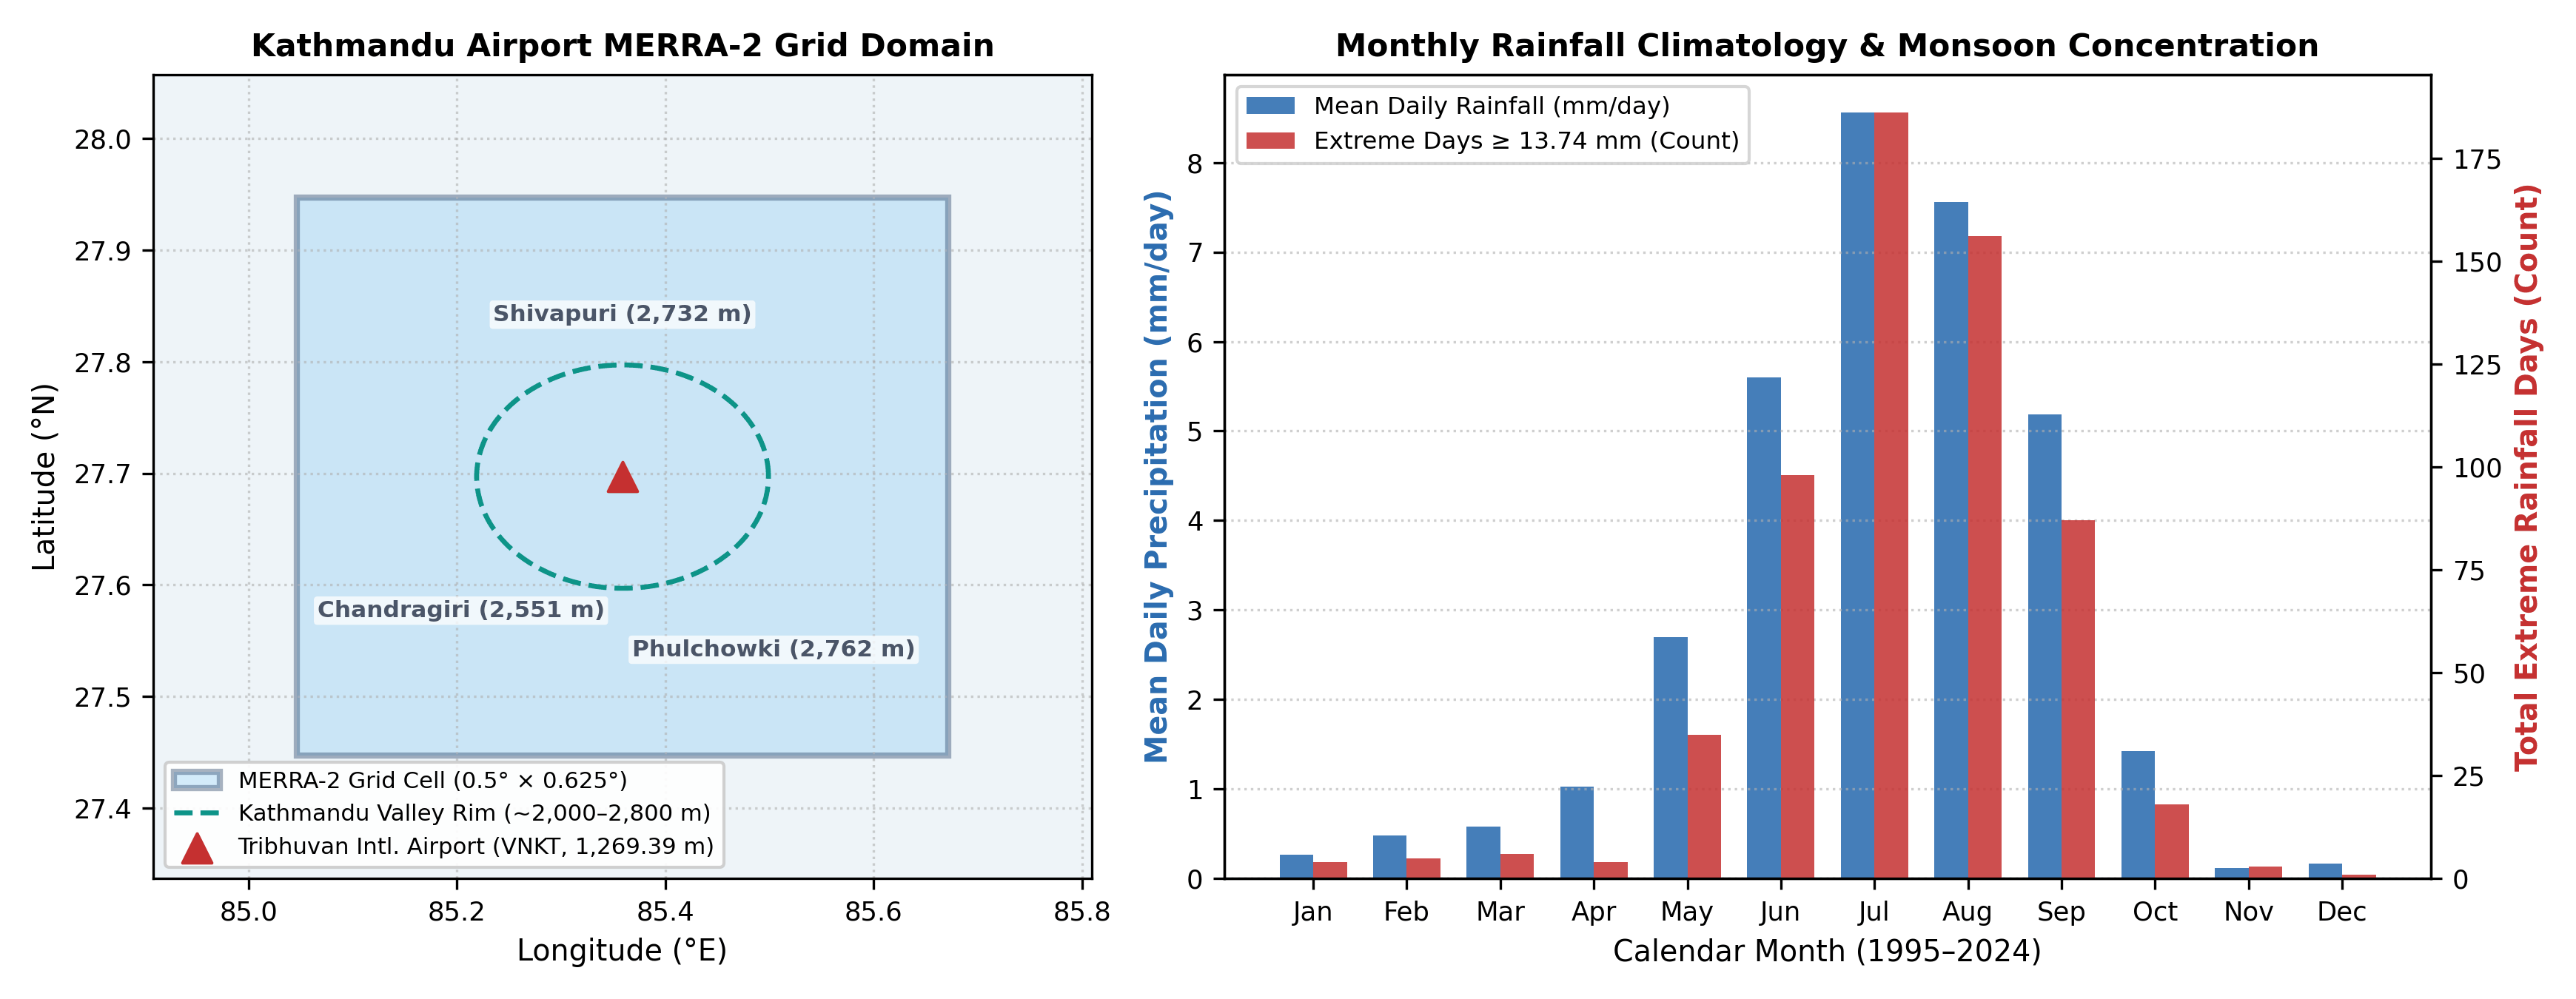
\includegraphics[width=\columnwidth]{figures/figure_01_location.png}
\caption{Study domain showing the NASA POWER MERRA-2 grid cell centred at Tribhuvan International Airport within the Kathmandu Valley rim (left), alongside the 1995--2024 monthly mean rainfall and extreme event counts (right).}
\label{fig:f1}
\end{figure}

\subsubsection{Chronological Train-Test Split and Data Quality Audit}
Trimming the first 7 dry winter days of January 1995 to initialise 7-day past rainfall totals leaves 10,951 complete daily records. To prevent temporal leakage, the dataset is split chronologically at 31 December 2018 into an 80\% training set (1995--2018, 8,759 days) and a 20\% holdout test set (2019--2024, 2,192 days), as shown in Table~\ref{tab:t1}. Table~\ref{tab:t2} summarises the 13 raw variables. Data checks confirmed zero missing dates, while post-2012 negative calm-wind placeholder codes (-8994.0 to -5404.0) in 10m wind direction were converted into a binary calm-wind indicator.

\begin{table}[H]
\caption{CHRONOLOGICAL DATASET PARTITIONS, SAMPLE SIZES, AND EXTREME RAINFALL COUNTS}
\label{tab:t1}
\centering
\resizebox{\columnwidth}{!}{%
\begin{tabular}{llll}
\toprule
\textbf{Dataset Partition} & \textbf{Date Range} & \textbf{All-Day Threshold (13.74 mm)} & \textbf{Wet-Day Threshold (22.75 mm)} \\
\midrule
Raw Archive & 1995-01-01 to 2024-12-31 & 10,958 days (603 extremes) & 10,958 days (212 extremes) \\
Lag Trim Window & 1995-01-01 to 1995-01-07 & 7 winter days (0 extremes) & 7 winter days (0 extremes) \\
Complete Modelling Set & 1995-01-08 to 2024-12-31 & 10,951 days (603 extremes, 5.51\%) & 10,951 days (212 extremes, 1.94\%) \\
\textbf{Training Set (80\%)} & \textbf{1995-01-08 to 2018-12-31} & \textbf{8,759 days (439 extremes, 5.01\%)} & \textbf{8,759 days (148 extremes, 1.69\%)} \\
\textbf{Holdout Test Set (20\%)} & \textbf{2019-01-01 to 2024-12-31} & \textbf{2,192 days (164 extremes, 7.48\%)} & \textbf{2,192 days (64 extremes, 2.92\%)} \\
\bottomrule
\end{tabular}%
}
\end{table}

\begin{table}[H]
\caption{RAW METEOROLOGICAL VARIABLES AND TRAINING SUMMARY STATISTICS (1995--2018, 8,759 DAYS)}
\label{tab:t2}
\centering
\resizebox{\columnwidth}{!}{%
\begin{tabular}{lllcc}
\toprule
\textbf{Variable} & \textbf{Units} & \textbf{Physical Weather Role} & \textbf{Train Mean $\pm$ SD} & \textbf{Min / Max} \\
\midrule
PRECTOTCORR & mm/day & Daily total rainfall (target source) & 2.59 $\pm$ 5.72 & 0.00 / 60.01 \\
T2M & $^\circ$C & Mean 2m air temperature & 19.22 $\pm$ 4.98 & 4.11 / 30.11 \\
T2M\_MAX & $^\circ$C & Maximum daily 2m temperature & 24.72 $\pm$ 4.64 & 9.93 / 37.30 \\
T2M\_MIN & $^\circ$C & Minimum daily 2m temperature & 15.10 $\pm$ 5.08 & -0.12 / 24.91 \\
T2MDEW & $^\circ$C & Dew point temperature at 2m & 8.78 $\pm$ 9.35 & -16.63 / 22.26 \\
RH2M & \% & Relative humidity at 2m & 57.31 $\pm$ 23.06 & 5.43 / 96.45 \\
QV2M & g/kg & Specific humidity (water vapour) & 9.67 $\pm$ 5.38 & 0.97 / 19.56 \\
PS & kPa & Surface air pressure & 87.27 $\pm$ 0.40 & 85.92 / 88.20 \\
WS10M & m/s & Mean 10m wind speed & 2.17 $\pm$ 0.52 & 0.86 / 4.65 \\
WS10M\_MAX & m/s & Peak daily 10m wind gust & 4.49 $\pm$ 1.02 & 1.72 / 9.55 \\
WD10M$^*$ & Degrees & 10m wind direction (non-calm days) & 217.8 $\pm$ 43.7 & 1.20 / 359.9 \\
ALLSKY\_SW & MJ/m$^2$/d & Downward solar radiation & 17.60 $\pm$ 4.69 & 2.21 / 30.54 \\
TS & $^\circ$C & Surface skin temperature & 18.46 $\pm$ 6.43 & 2.60 / 31.46 \\
\bottomrule
\end{tabular}%
}
\vspace{1.5pt}
{\scriptsize\raggedright $^*$Note: Post-2012 negative calm-wind codes in WD10M are captured via a binary calm-wind indicator.\par}
\end{table}

\subsection{Target Thresholds and Operational Classification Tasks}

\subsubsection{Extreme Rainfall Thresholds (13.74 mm and 22.75 mm)}
Two extreme rainfall thresholds are calculated strictly from the 1995--2018 training set \cite{ref3,ref4}: the all-day 95th percentile (13.74 mm/day, giving 439 training extremes at 5.01\% and 164 test extremes at 7.48\%) and the wet-day 95th percentile across days with at least 1.0 mm of rain (22.75 mm/day, giving 148 training and 64 test deluges), as plotted in Fig.~\ref{fig:f2}.

\begin{figure}[H]
\centering
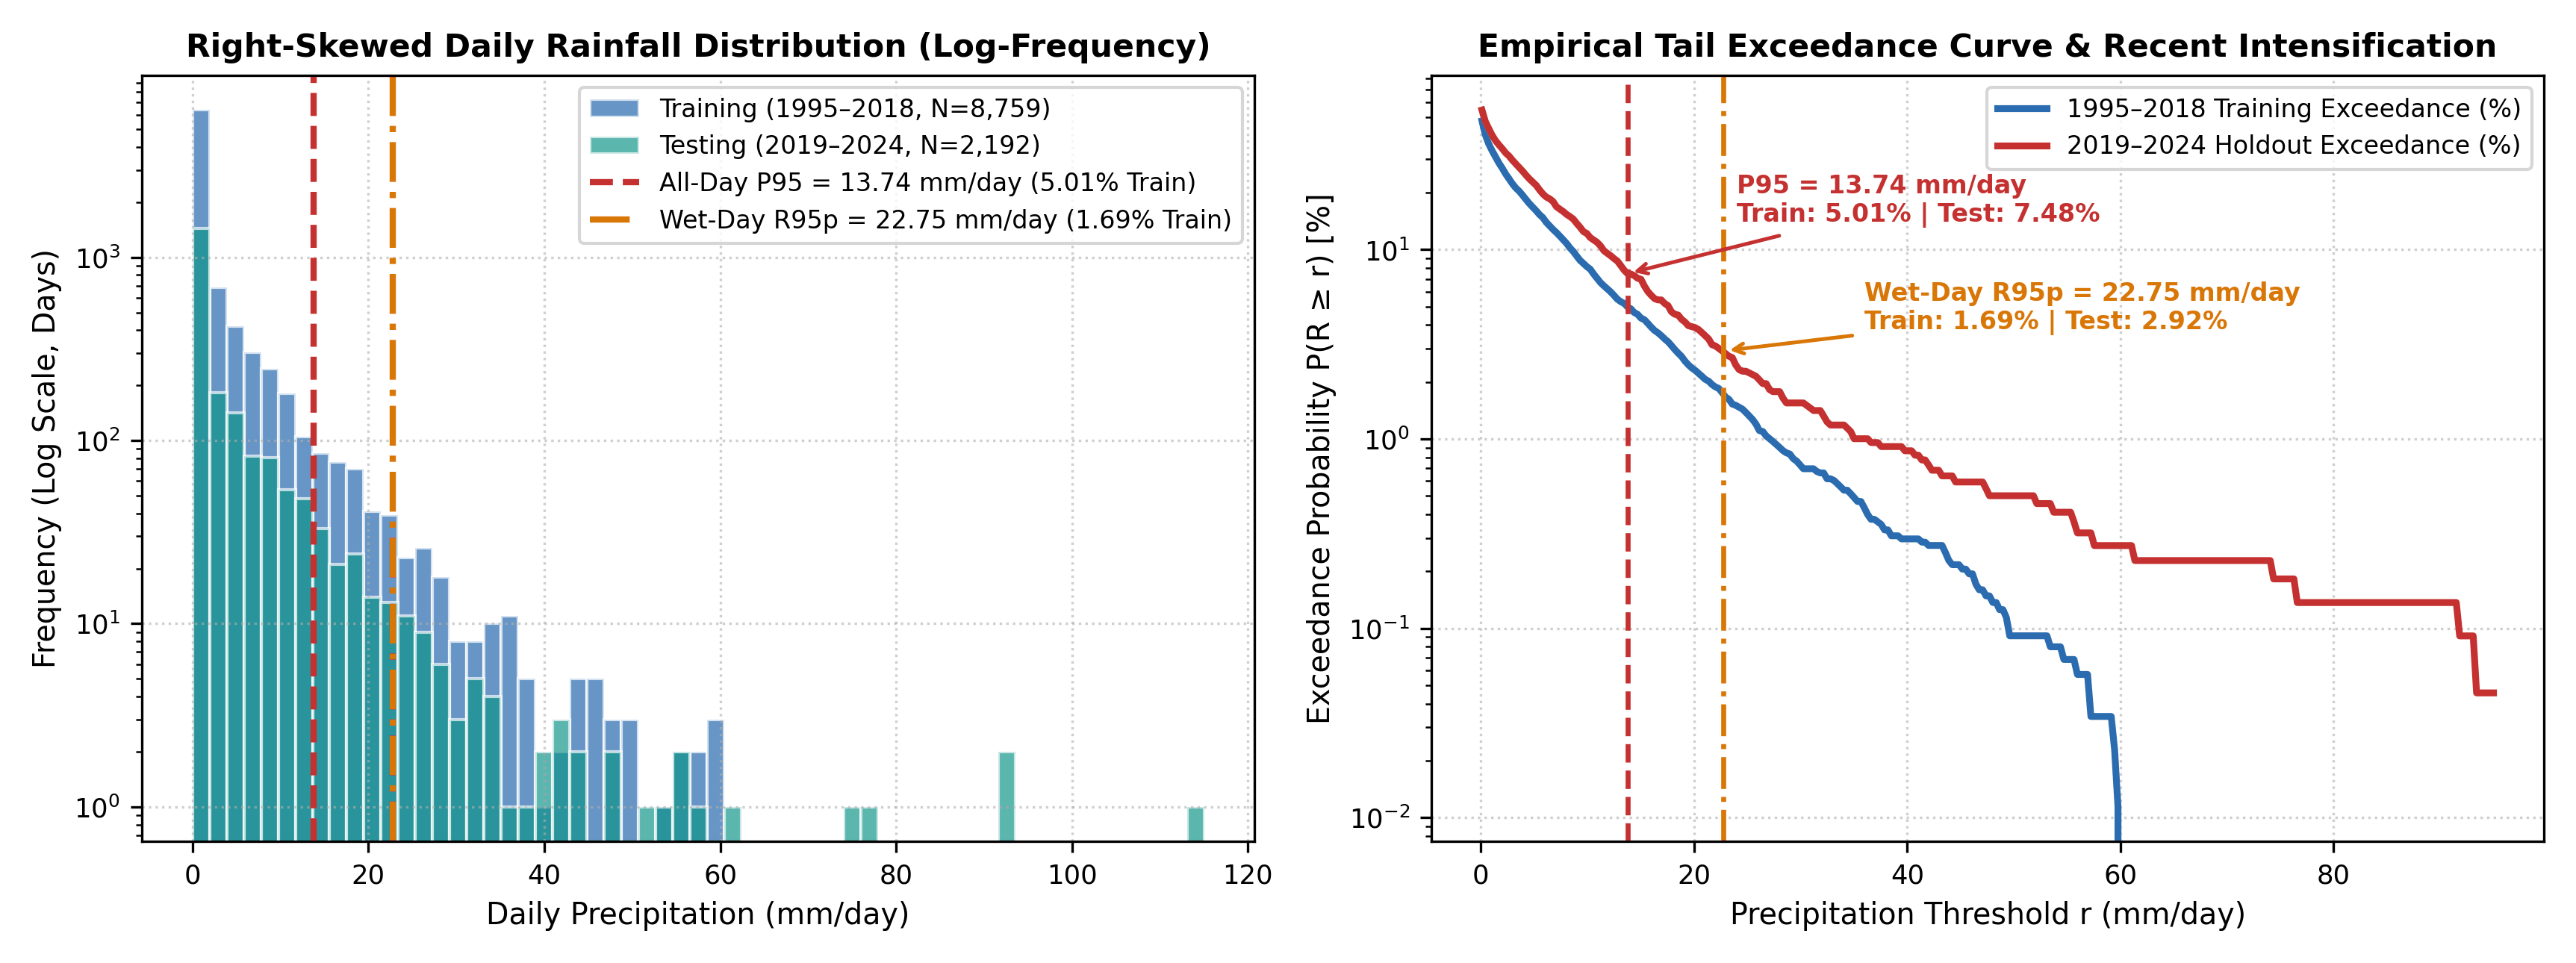
\includegraphics[width=\columnwidth]{figures/figure_02_tail_distribution.png}
\caption{Daily rainfall frequency distribution (left) and exceedance probability curves comparing the 1995--2018 training period against the 2019--2024 holdout period (right) at the 13.74 mm/day and 22.75 mm/day thresholds.}
\label{fig:f2}
\end{figure}

\subsubsection{Operational Classification Tasks (Tasks A, B, and C)}
To evaluate both same-day weather diagnosis and true advance warning under RO3, three classification tasks are defined:
\begin{itemize}
  \setlength{\itemsep}{1.5pt}\setlength{\parskip}{0pt}
  \item \textbf{Task A (Same-Day Atmospheric State Classification at 13.74 mm/day):} Uses same-day non-rainfall weather conditions (humidity, temperature, pressure, wind, and solar radiation) together with 1-to-7-day past rainfall to diagnose whether that same day experiences extreme rainfall ($\ge 13.74$ mm/day).
  \item \textbf{Task B (Strict 24-Hour Advance Forecasting at 13.74 mm/day):} Shifts all 15 weather state variables back by one full day so that only observations recorded on or before yesterday are used to forecast tomorrow's extreme rainfall a full 24 hours in advance.
  \item \textbf{Task C (Severe Wet-Day Deluge Classification at 22.75 mm/day):} Evaluates classifier ability to detect severe wet-day downpours exceeding the 22.75 mm/day threshold.
\end{itemize}

\section{Methods and Experimental Setup}

\subsection{Experimental Setup, Data Pre-Processing, and Feature Extraction}

\subsubsection{Leak-Free Pre-Processing and Feature Extraction Pipeline}
Fig.~\ref{fig:f3} shows the leak-free workflow and 5-fold expanding-window time-series validation design, and Table~\ref{tab:t3} lists the 22 engineered predictors. Inside each training fold, continuous weather predictors are standardised using z-score normalisation so that variables measured in different units share a common scale:
\begin{equation}
z_{i,j} = \frac{x_{i,j} - \mu_j}{\sigma_j}
\end{equation}
where $x_{i,j}$ is the raw value of feature $j$ on day $i$, and $\mu_j$ and $\sigma_j$ are the mean and standard deviation calculated strictly from the historical training records.

\begin{figure}[H]
\centering
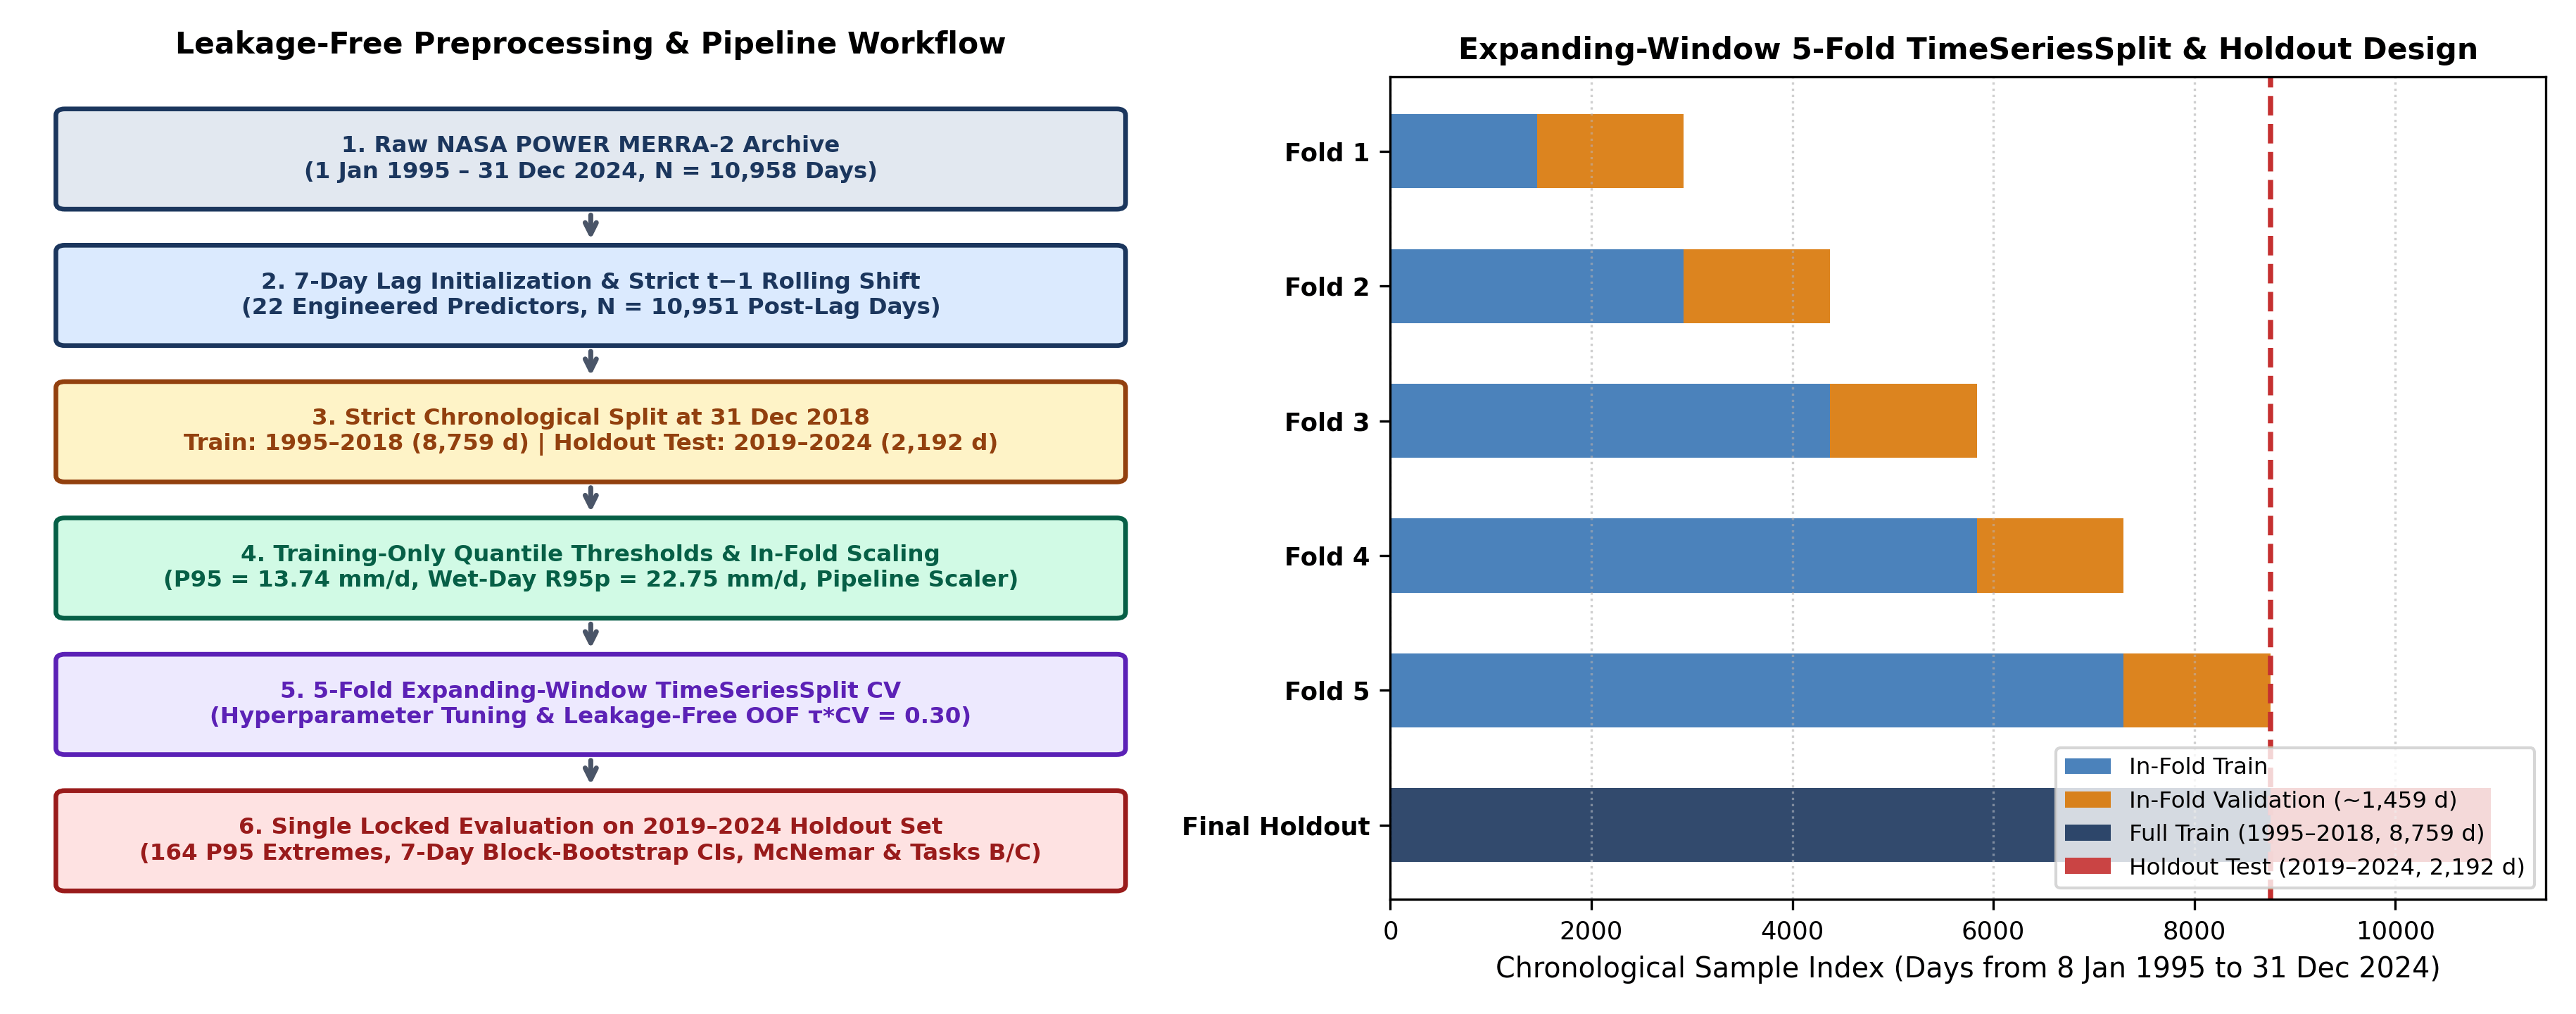
\includegraphics[width=\columnwidth]{figures/figure_03_workflow_cv.png}
\caption{Leak-free data preparation and evaluation workflow (left) and the 5-fold expanding-window time-series validation schedule applied strictly within the 1995--2018 training set (right).}
\label{fig:f3}
\end{figure}

\begin{table}[H]
\caption{INVENTORY OF THE 22 ENGINEERED WEATHER PREDICTORS}
\label{tab:t3}
\centering
\resizebox{\columnwidth}{!}{%
\begin{tabular}{clll}
\toprule
\textbf{\#} & \textbf{Predictor Name} & \textbf{Calculation Method and Units} & \textbf{Physical Weather Meaning} \\
\midrule
1 & T2M & Daily mean 2m air temperature ($^\circ$C) & Warmth governing moisture capacity \\
2 & T2M\_MAX & Daily maximum 2m temperature ($^\circ$C) & Daytime surface heating peak \\
3 & T2M\_MIN & Daily minimum 2m temperature ($^\circ$C) & Nighttime cloud heat trapping \\
4 & temp\_diurnal\_range & Max minus min daily temperature ($^\circ$C) & Cloud cooling (narrows on rainy days) \\
5 & T2MDEW & Dew point temperature at 2m ($^\circ$C) & Condensation temperature threshold \\
6 & dew\_point\_depression & Air temperature minus dew point ($^\circ$C) & Near-surface air saturation gap \\
7 & RH2M & Relative humidity at 2m (\%) & Near-surface moisture saturation \\
8 & QV2M & Specific humidity at 2m (g/kg) & Water vapour fuel for storm clouds \\
9 & PS & Surface atmospheric pressure (kPa) & Monsoon low-pressure trough depth \\
10 & pressure\_tendency & Today minus yesterday pressure (kPa) & 24-hour barometric rise or fall \\
11 & WS10M & Mean 10m wind speed (m/s) & Valley moisture transport speed \\
12 & WS10M\_MAX & Maximum daily 10m wind gust (m/s) & Storm downdraught gust strength \\
13 & ALLSKY\_SW & Downward solar radiation (MJ/m$^2$/d) & Sunlight blocked by storm clouds \\
14 & TS & Surface skin temperature ($^\circ$C) & Land-surface heating state \\
15 & wind\_calm\_flag & Binary flag for negative wind code (0/1) & Calm or variable valley wind state \\
16 & precip\_lag1 & Rainfall 1 day ago (mm/day) & Yesterday's rainfall persistence \\
17 & precip\_lag2 & Rainfall 2 days ago (mm/day) & 48-hour storm track memory \\
18 & precip\_lag3 & Rainfall 3 days ago (mm/day) & 72-hour wet spell persistence \\
19 & precip\_roll3 & Total rainfall over past 3 days (mm) & Short-term soil and air wetting \\
20 & precip\_roll7 & Total rainfall over past 7 days (mm) & Weekly catchment moisture build-up \\
21 & sin\_doy & Sine wave of calendar day of year & Smooth seasonal progression (spring/autumn) \\
22 & cos\_doy & Cosine wave of calendar day of year & Smooth winter-to-monsoon cycle \\
\bottomrule
\end{tabular}%
}
\end{table}

\subsection{Unsupervised Pattern Analysis and Clustering Methods (RO1)}

\subsubsection{Principal Component Analysis (PCA)}
PCA is selected to measure overlap among the 22 predictors and test whether compressing them into uncorrelated axes retains extreme rain signals \cite{ref17}. It is fitted strictly on the standardised 1995--2018 training matrix (8,759 days across 22 features) without access to rainfall labels or test data. Configured in Scikit-learn with random seed 42 (fit time 0.0028 s, Table~\ref{tab:t4}), the number of retained components $m$ is selected using the cumulative explained variance ratio:
\begin{equation}
\text{EVR}_m = \frac{\sum_{k=1}^{m} \lambda_k}{\sum_{j=1}^{22} \lambda_j} \ge 0.90
\end{equation}
where $\lambda_k$ is the eigenvalue of component $k$, which retains $m = 7$ components explaining 91.46\% of total training variance. PCA advances RO1 by isolating monsoon moisture saturation (Component 1, 42.29\%) and solar heating (Component 2, 24.17\%), but compressing 22 features into 7 components reduces downstream storm recall because global variance smoothing blurs sharp 1-day rain spikes.

\subsubsection{Fast Independent Component Analysis (FastICA)}
FastICA is selected as an exploratory diagnostic method to separate sharp, non-normal storm spikes from smooth seasonal cycles. It is applied to the standardised 8,759-day training table after 7-component whitening as an unsupervised diagnostic tool rather than a supervised classifier, configured in Scikit-learn with 7 components, a log-cosh contrast function, 500 maximum iterations, and seed 42 (fit time 0.1383 s, Table~\ref{tab:t4}). This supports RO1 by separating the post-2012 calm-wind shift from sharp multi-day rain bursts, though its unitless axes are less interpretable than physical features for tree splits.

\subsubsection{K-Means Clustering}
K-Means clustering is selected to group daily valley weather states into objective seasonal regimes and measure storm concentration \cite{ref17}. It is applied to the unlabelled standardised training matrix across 2 to 6 candidate clusters before comparing cluster assignments against historical storm labels, configured in Scikit-learn with 3 clusters, 10 initialisations, and seed 42 (fit time 0.0804 s, Table~\ref{tab:t4}) to partition daily weather states by minimising the Within-Cluster Sum of Squares (WCSS):
\begin{equation}
J_{\text{WCSS}} = \sum_{k=1}^{K} \sum_{z_i \in C_k} \| z_i - \mu_k \|_2^2
\end{equation}
where $C_k$ is weather regime cluster $k$ and $\mu_k$ is its cluster centre across the 22 standardised features. K-Means advances RO1 by identifying an Active Saturated Monsoon cluster that captures 94.99\% (417 of 439) of training storms, though 87.35\% of days in that cluster remain non-extreme, requiring supervised classifiers for precise warning.

\subsection{Supervised Classification Algorithms (RO2 and RO3)}

\subsubsection{Logistic Regression}
Logistic Regression is selected as an interpretable linear baseline to test weighted straight-line separation of extreme rain days \cite{ref18}. It is trained on all 22 standardised predictors inside an in-fold scaling pipeline and configured in Scikit-learn with L2 penalty, the LBFGS solver, balanced class weights (19-to-1 storm weighting), and a tuned regularisation strength of $C = 0.01$ (Table~\ref{tab:t5}), minimising the weighted cross-entropy loss function:
\begin{equation}
L_{\text{LR}} = -\frac{1}{N}\sum_{i=1}^{N}\left[w_1 y_i \ln(\hat{p}_i) + w_0(1-y_i)\ln(1-\hat{p}_i)\right] + \frac{\|w\|_2^2}{2C}
\end{equation}
where $\hat{p}_i$ is the predicted storm probability on day $i$, and $w_1 = 9.98$ and $w_0 = 0.53$ are the inverse-frequency class weights that counter the 1-to-19 imbalance. Logistic Regression achieves the highest test storm recall (96.34\%, 158 of 164 storms, ROC-AUC 0.9411), but its flat boundary flags 523 humid monsoon days as false alarms (23.20\% precision).

\subsubsection{Decision Tree (CART)}
Decision Tree (CART) is selected as a rule-based baseline that splits weather variables along clear step thresholds \cite{ref16}. Trained on the 22 unscaled physical features so split rules remain readable in original physical units, it is configured in Scikit-learn with Gini impurity, balanced class weights, maximum depth 8, minimum split 10, and minimum leaf size 5 (Table~\ref{tab:t5}). On the holdout test set, CART reaches 85.98\% recall and an F1-score of 0.4046, but suffers from single-feature dominance by placing 73.35\% of its total decision weight on yesterday's rainfall alone.

\subsubsection{Radial Basis Function Support Vector Machine (RBF-SVM)}
RBF-SVM is selected to test whether a smooth, curved kernel boundary improves storm separation over linear and single-tree models \cite{ref2}. Trained on the 22 standardised predictors inside an in-fold scaling pipeline, it is configured in Scikit-learn with an RBF kernel, penalty C of 1.0, automatic kernel scaling, balanced weights, and Platt probability calibration (Table~\ref{tab:t5}). RBF-SVM achieves the best probability calibration (Brier 0.0553) and 87.80\% recall, but trails Random Forest in Precision-Recall AUC (0.3676) and requires the longest training time (10.45 s).

\subsubsection{Random Forest}
Random Forest is selected as a bagged tree ensemble designed to prevent single-variable overfitting and reduce false alarms \cite{ref1,ref18,ref19}. Trained on the 22 physical predictors across 100 bootstrap trees while restricting each split to 4 randomly chosen candidate features, it is configured in Scikit-learn with 100 trees, maximum depth 8, minimum leaf size 5, balanced class weights, and seed 42 (fit time 1.29 s, Table~\ref{tab:t4} and Table~\ref{tab:t5}). Random Forest delivers the best overall balance on the holdout set (F1 of 0.4385, Precision-Recall AUC 0.5517, ROC-AUC 0.9349, and 90.24\% recall), with only minor first-day lag delay after dry spells.

\subsubsection{k-Nearest Neighbours (k-NN)}
k-NN is selected as a distance-based baseline to test whether matching days to closest historical weather records works under class skew \cite{ref2,ref20}. Trained on the 22 standardised predictors using straight-line Euclidean distance and configured in Scikit-learn with 5 nearest neighbours and uniform voting (Table~\ref{tab:t5}), k-NN exposes the accuracy paradox: despite 93.16\% overall accuracy, it misses 71.34\% of extreme storms (28.66\% recall) because non-extreme days dominate local 5-day neighbourhoods.

\subsection{Validation and Cost-Sensitive Threshold Design}

\subsubsection{Time-Series Cross-Validation and Evaluation Metrics}
All models are tuned via 5-fold expanding-window time-series cross-validation on 1995--2018 (Table~\ref{tab:t4} and Table~\ref{tab:t5}). Because overall accuracy is misleading on imbalanced data, models are evaluated using Precision, Recall, the harmonic $F_1$-score, and the Brier probability calibration score (BS):
\begin{equation}
\begin{aligned}
\text{Prec} &= \frac{\text{TP}}{\text{TP}+\text{FP}}, \quad \text{Rec} = \frac{\text{TP}}{\text{TP}+\text{FN}}, \\
F_1 &= \frac{2\,\text{TP}}{2\,\text{TP}+\text{FP}+\text{FN}}, \quad \text{BS} = \frac{1}{N}\sum_{i=1}^{N}(\hat{p}_i - y_i)^2
\end{aligned}
\end{equation}
where TP, FP, and FN denote true positives, false positives, and false negatives.

\subsubsection{Asymmetric 15-to-1 Disaster Cost Function}
Under RO3, decision thresholds $\tau$ from 0.05 to 0.95 are evaluated using an asymmetric 15-to-1 \textbf{missed-storm cost function} that weights each missed flood 15 times more heavily than a false alarm:
\begin{equation}
\text{Cost}(\tau) = 15 \times \text{FN}(\tau) + 1 \times \text{FP}(\tau)
\end{equation}
selecting the operational threshold of 0.30 strictly from out-of-fold training predictions without viewing the holdout test set.

\begin{table}[H]
\caption{TRAINING RUNTIMES, TEST INFERENCE SPEED, AND SCALING BEHAVIOUR ACROSS ALL EIGHT ALGORITHMS}
\label{tab:t4}
\centering
\resizebox{\columnwidth}{!}{%
\begin{tabular}{llll}
\toprule
\textbf{Method / Classifier} & \textbf{Scaling Behaviour} & \textbf{Train Fit Time} & \textbf{Test Inference (2,192 d)} \\
\midrule
PCA (22 features) & Fast matrix decomposition & 0.0028 s & Not applicable \\
FastICA (7 components) & Fast iterative projection & 0.1383 s & Not applicable \\
K-Means (3 clusters) & Fast centroid distance updates & 0.0804 s & Not applicable \\
Logistic Regression & Fast linear gradient optimisation & 0.0533 s & 0.0011 s \\
Decision Tree (CART) & Fast single-tree threshold sorting & 0.0576 s & 0.0006 s \\
RBF-Kernel SVM & Slow pairwise kernel optimization & 10.4518 s & 0.7772 s \\
\textbf{Random Forest (100 trees)} & \textbf{Moderate parallel tree building} & \textbf{1.2909 s} & \textbf{0.0290 s} \\
k-NN (5 neighbours) & Instant storage; slow test distance scan & 0.0024 s & 0.0702 s \\
\bottomrule
\end{tabular}%
}
\end{table}

\begin{table}[H]
\caption{FIVE-FOLD TIME-SERIES CROSS-VALIDATION SEARCH GRIDS AND SELECTED MODEL CONFIGURATIONS}
\label{tab:t5}
\centering
\resizebox{\columnwidth}{!}{%
\begin{tabular}{lllc}
\toprule
\textbf{Classifier} & \textbf{Candidate Settings Tested} & \textbf{Selected Best Configuration} & \textbf{Train CV F1 ($\pm$ SD)} \\
\midrule
Logistic Regression & Penalty C: 0.01, 0.1, 1.0, 10.0 & C = 0.01, L2 penalty, balanced weights & 0.3172 $\pm$ 0.0778 \\
Decision Tree (CART) & Depth: 3, 4, 5, 6, 8; Leaf: 5, 10, 20 & Max depth = 8, min leaf = 5, balanced & 0.3383 $\pm$ 0.0566 \\
RBF-Kernel SVM & Penalty C: 0.5, 1.0, 2.0; scale kernel & C = 1.0, RBF kernel, balanced, Platt & 0.3476 $\pm$ 0.0514 \\
\textbf{Random Forest} & \textbf{Trees: 100, 150; Depth: 4, 6, 8; Leaf: 5, 10} & \textbf{100 trees, max depth = 8, min leaf = 5} & \textbf{0.3780 $\pm$ 0.0429} \\
k-NN & Neighbours: 5, 9, 15, 21; uniform/distance & 5 neighbours, uniform voting & 0.2003 $\pm$ 0.0844 \\
\bottomrule
\end{tabular}%
}
\end{table}

\section{Results}

\subsection{Unsupervised Regime Findings (RO1)}

\subsubsection{Optimal Cluster Selection}
Applying PCA, FastICA, and K-Means to the 1995--2018 training set (8,759 days across 22 features) reveals clear seasonal weather structure in the Kathmandu Valley. As shown in Fig.~\ref{fig:f4}, testing cluster counts from 2 to 6 identifies a clear optimum at 3 clusters, where the Silhouette score reaches its global peak of 0.3119 and the Davies--Bouldin index reaches its lowest value of 1.1327. This confirms that daily Kathmandu weather naturally divides into three macro-seasonal regimes rather than an arbitrary number of groups.

\begin{figure}[H]
\centering
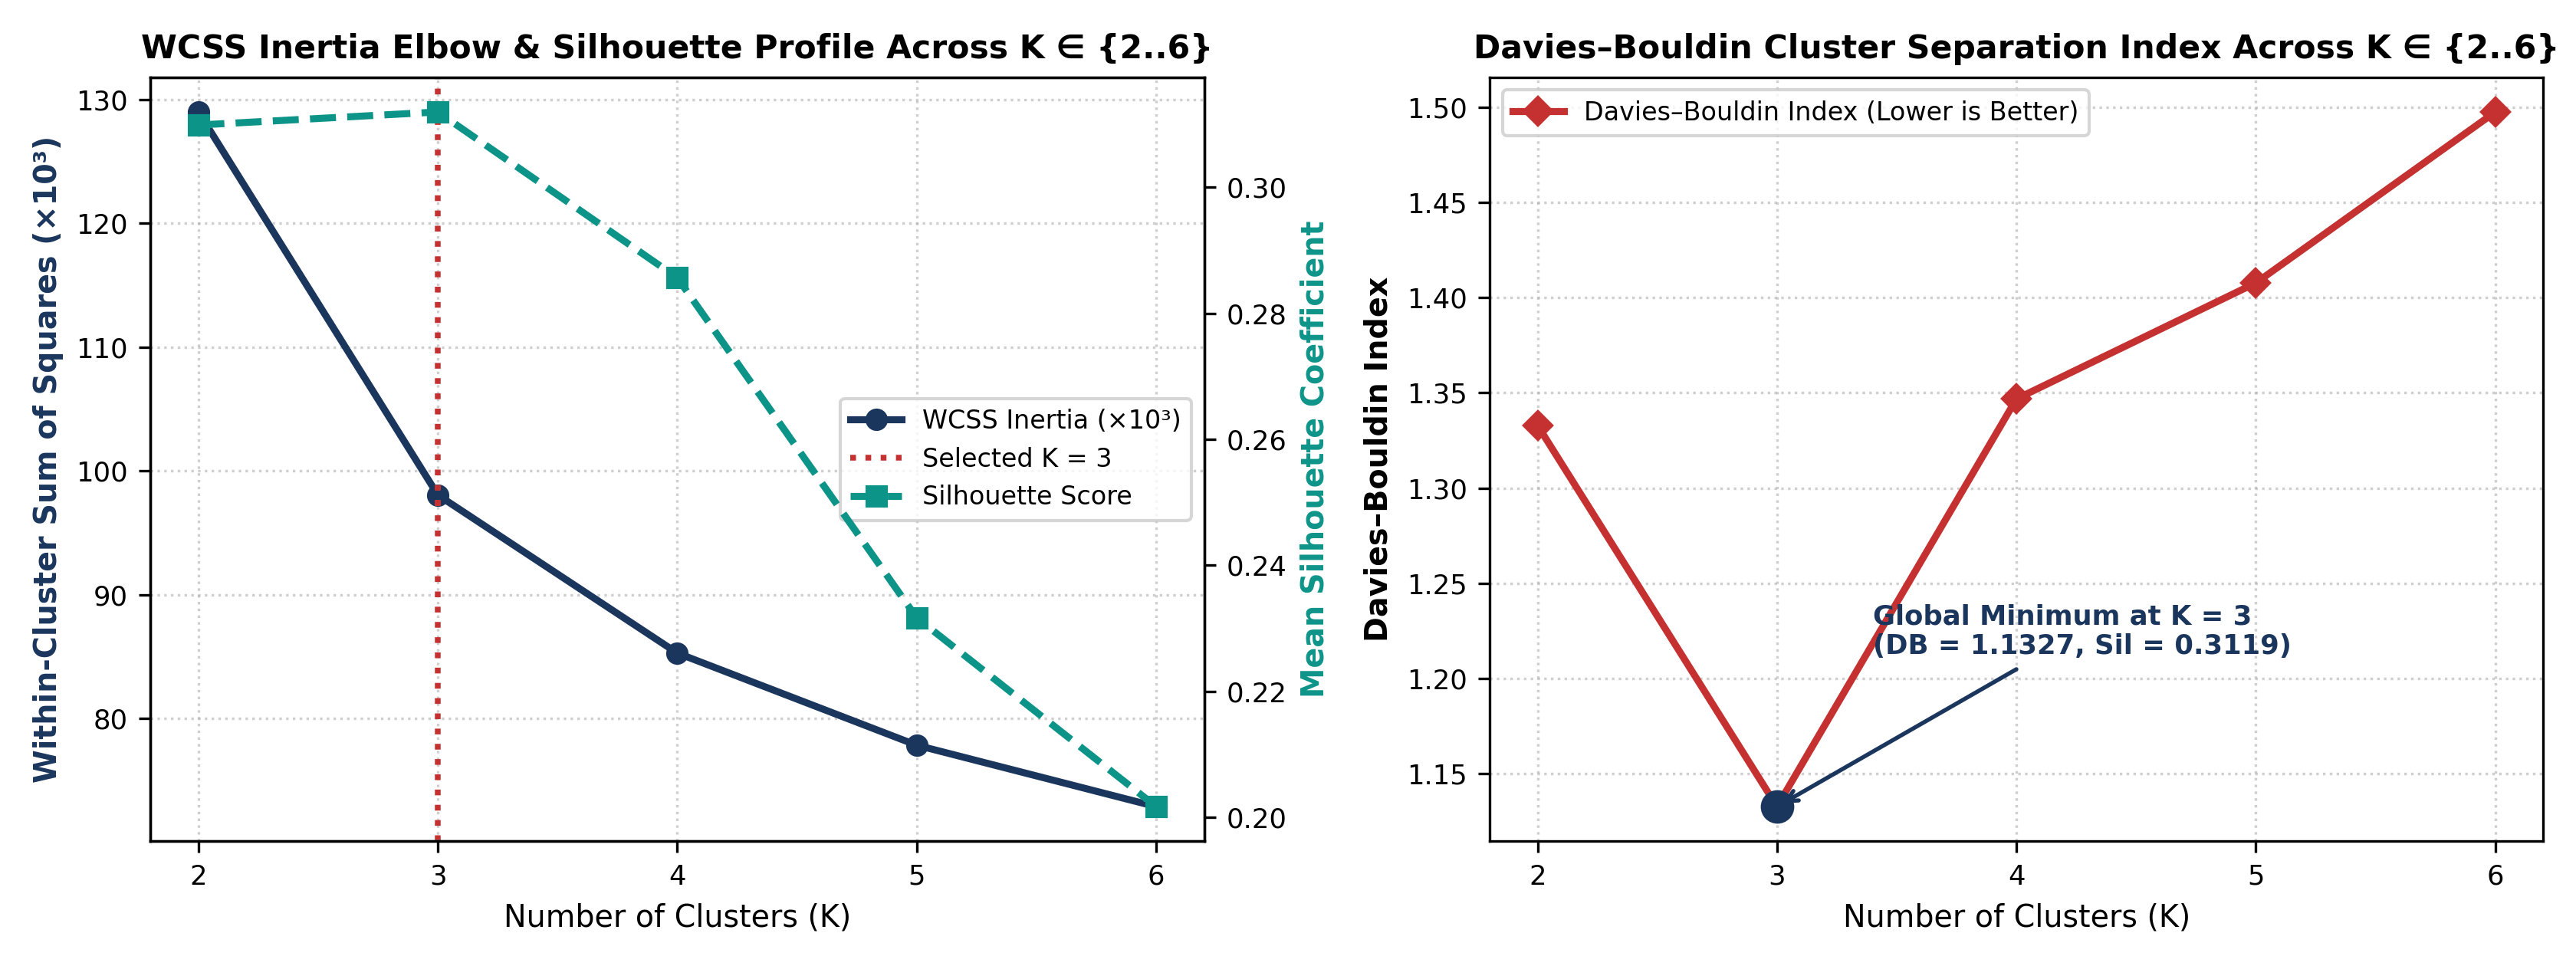
\includegraphics[width=\columnwidth]{figures/figure_04_kmeans_diagnostics.png}
\caption{Unsupervised K-Means cluster validation across 2 to 6 clusters on the 1995--2018 training set: inertia elbow and Silhouette peak at 3 clusters (left), and Davies--Bouldin minimum at 3 clusters (right).}
\label{fig:f4}
\end{figure}

\subsubsection{PCA and FastICA Component Structure}
Fig.~\ref{fig:f5} and Fig.~\ref{fig:f6} show how PCA and FastICA organise the 22 weather predictors. In Fig.~\ref{fig:f5} (left) and Fig.~\ref{fig:f6} (left), the first principal component accounts for 42.29\% of total training variance and is driven by high specific humidity (+0.313), high dew point (+0.307), warm nighttime minimum temperature (+0.282), high relative humidity (+0.265), and heavy 7-day past rainfall (+0.261), paired with low surface pressure (-0.245) and narrow daily temperature range (-0.233). Physically, this first axis represents warm, saturated monsoon low-pressure conditions. The second component explains 24.17\% of variance (bringing the two-axis total to 66.46\%) and reflects strong 10m wind speed (+0.360), high daytime temperature (+0.357), and bright solar radiation (+0.332) typical of clear pre-monsoon days. The third component (9.15\% variance) tracks 3-day and 2-day past rainfall persistence (+0.440 and +0.407). Together, the top 7 components retain 91.46\% of total variance (and 9 components retain 95.11\%). In Fig.~\ref{fig:f5} (right), FastICA separates the post-2012 calm-wind archive shift along its first axis while isolating sharp, heavy multi-day storm spikes along its second axis, confirming that extreme rain events stand out as distinct non-normal bursts.

\begin{figure}[H]
\centering
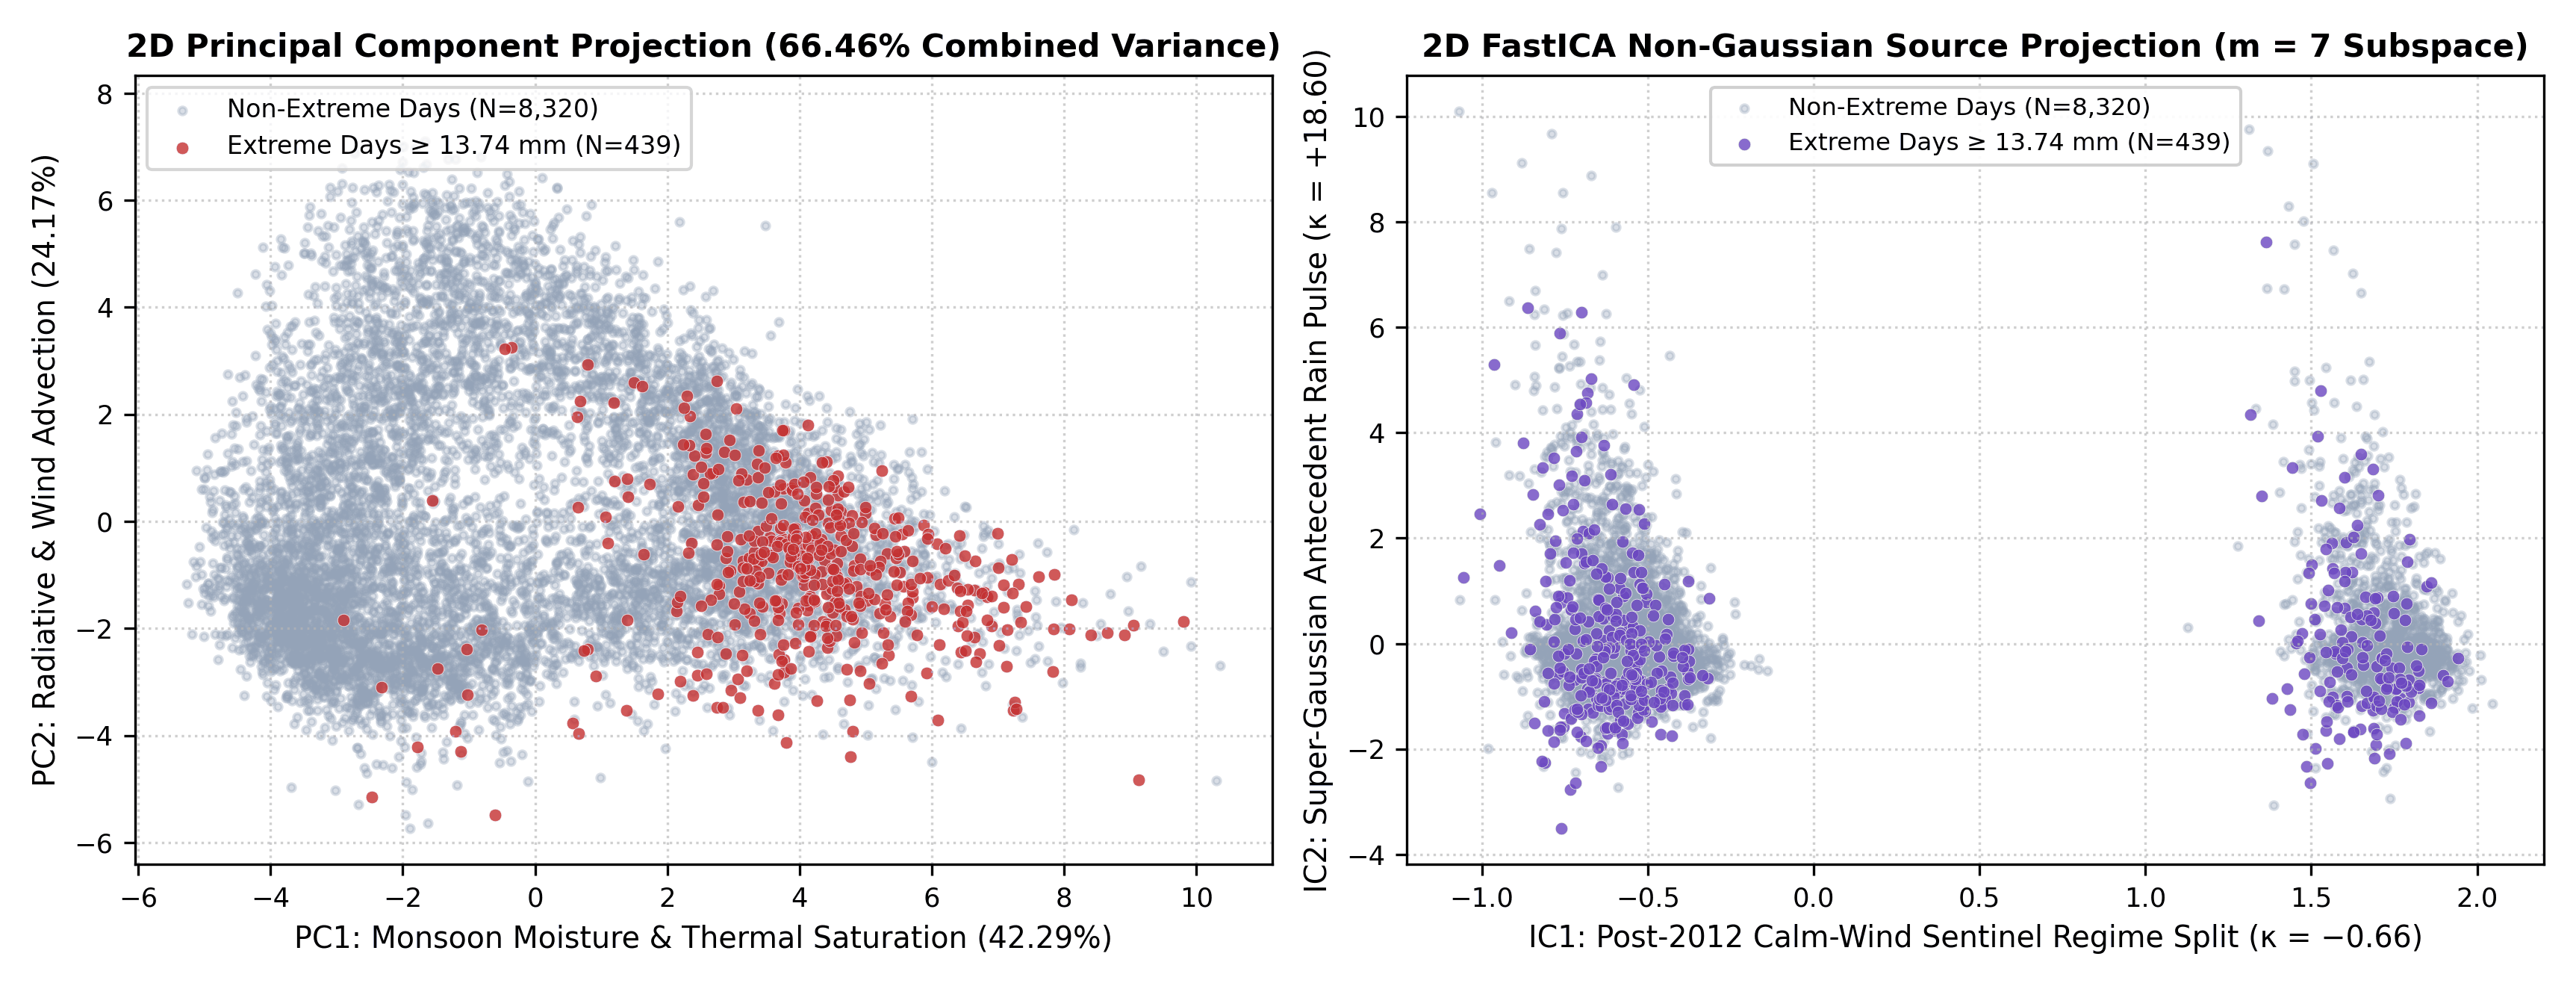
\includegraphics[width=\columnwidth]{figures/figure_05_pca_ica_projections.png}
\caption{Two-dimensional projections of the 22-feature training set coloured by extreme rainfall status: PCA projection capturing 66.46\% of variance (left) and FastICA independent source projection (right).}
\label{fig:f5}
\end{figure}

\begin{figure}[H]
\centering
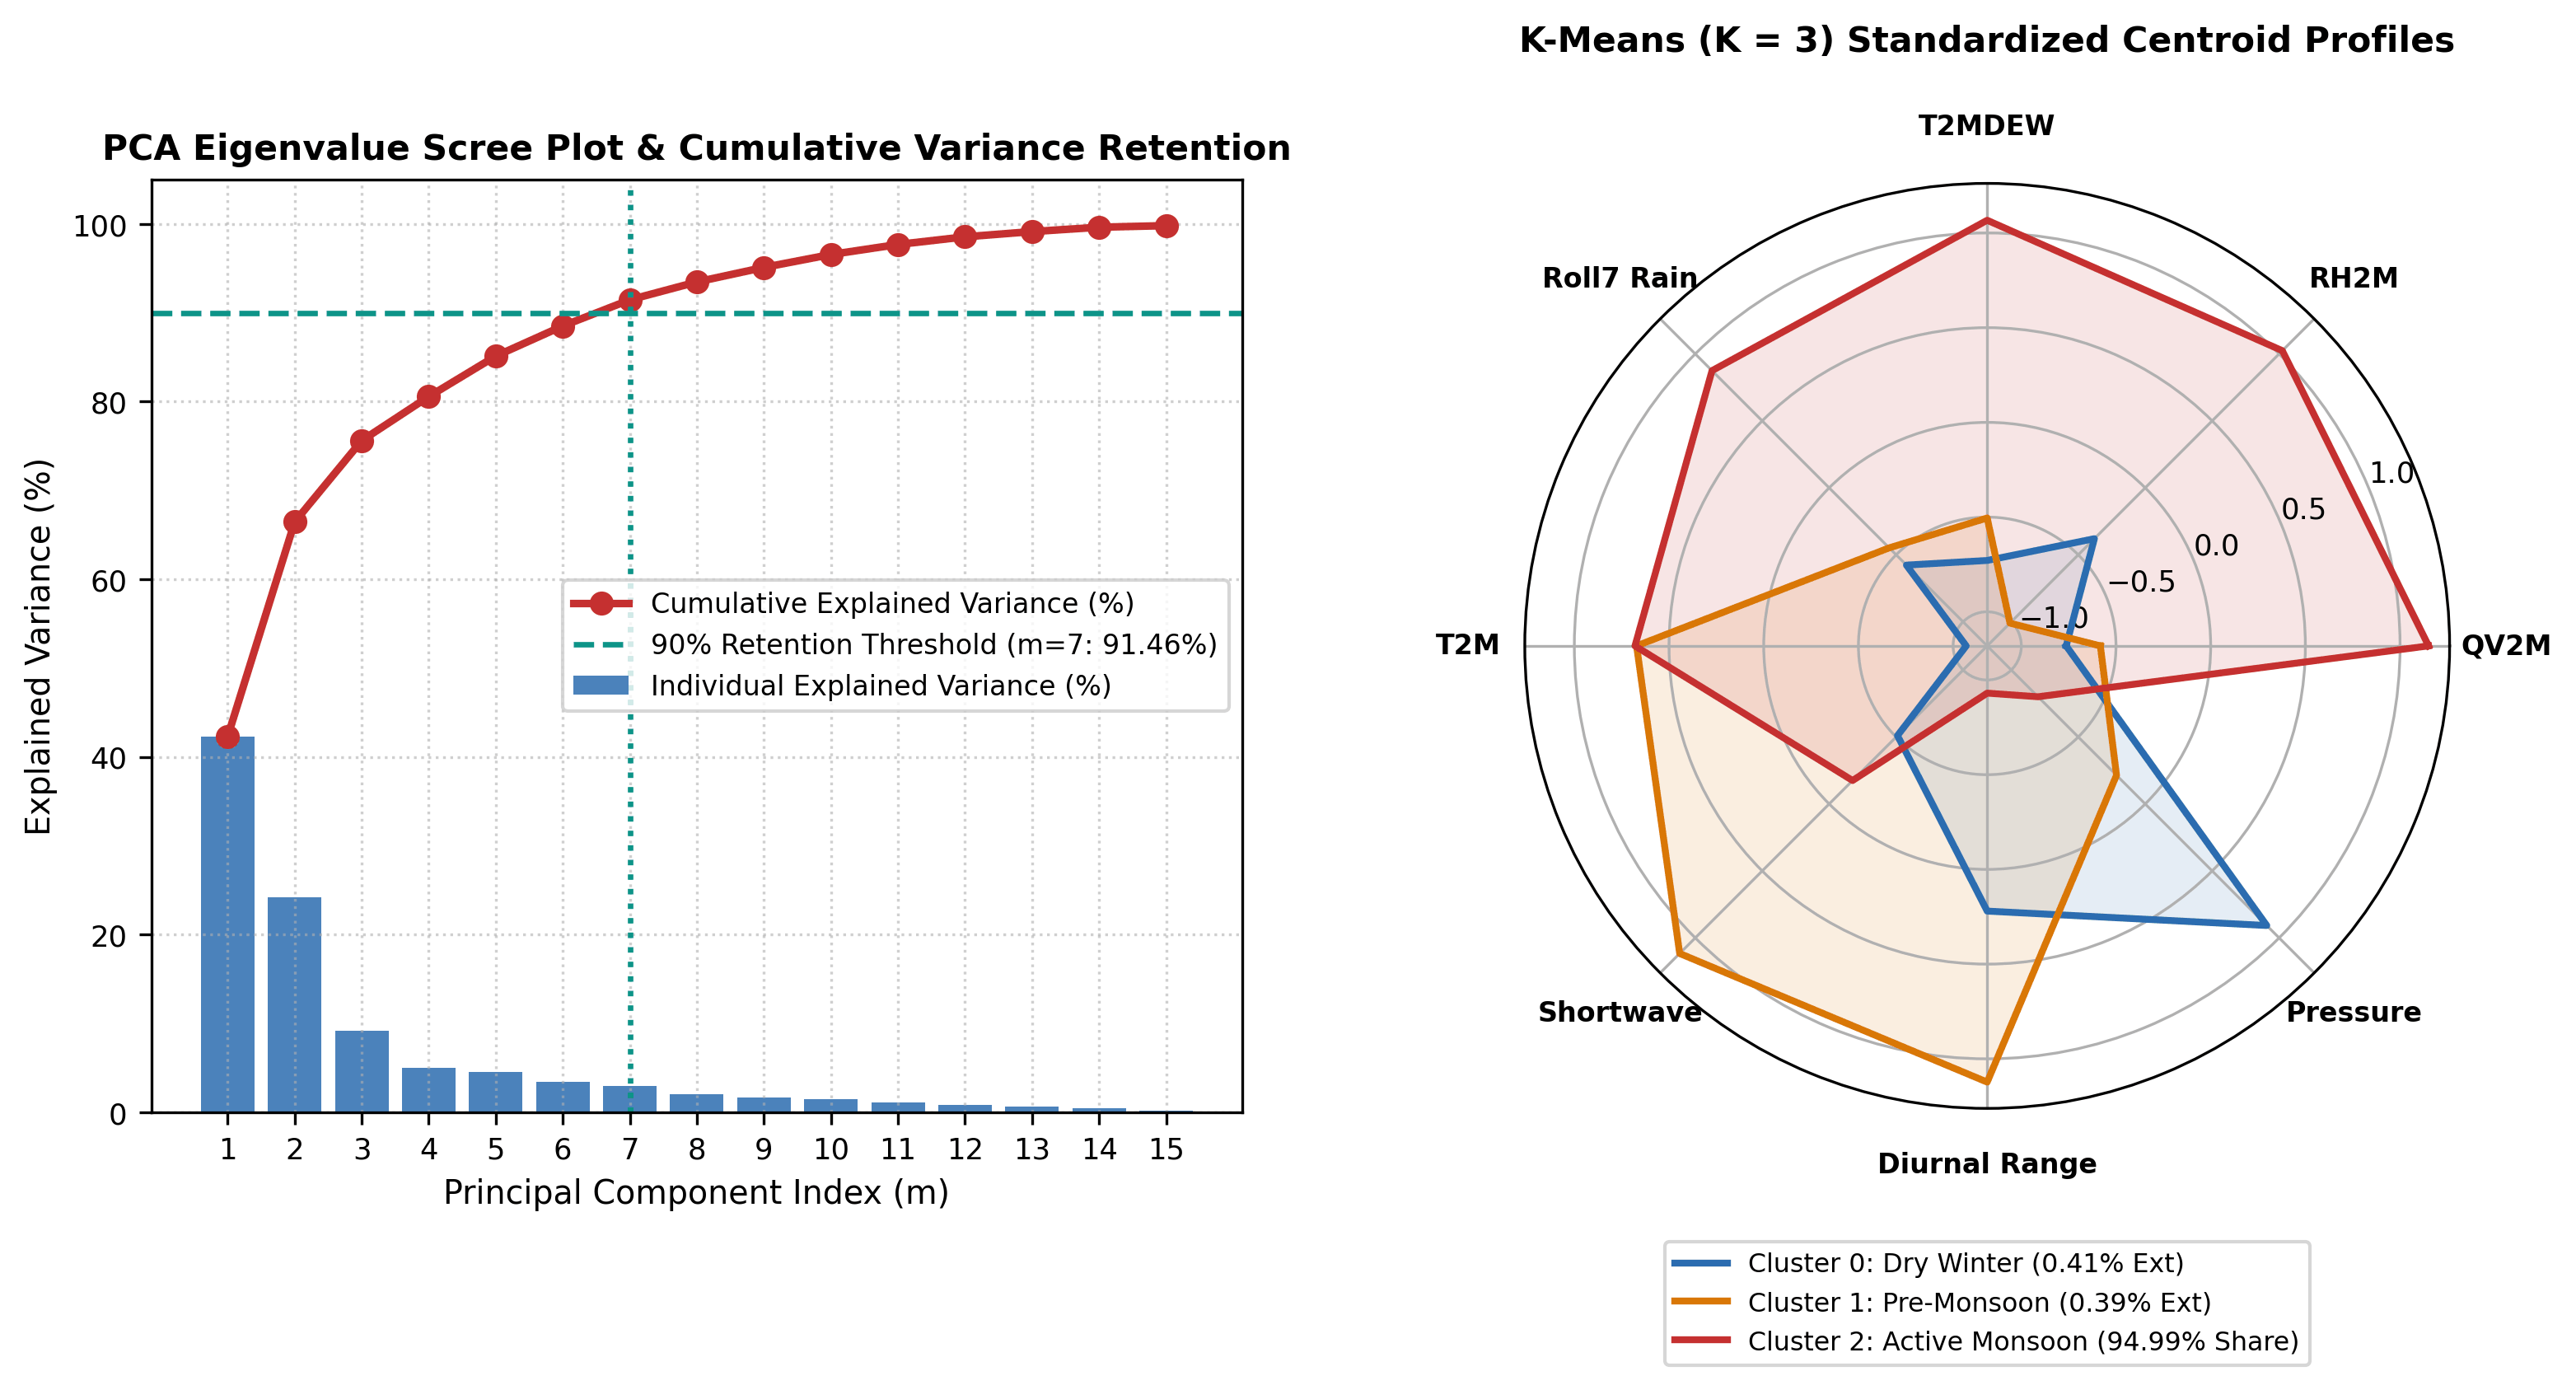
\includegraphics[width=\columnwidth]{figures/figure_06_pca_scree_kmeans_radar.png}
\caption{PCA explained variance scree plot showing 91.46\% retention at 7 components (left), paired with the K-Means (3 clusters) radar profile across eight core weather variables (right).}
\label{fig:f6}
\end{figure}

\subsubsection{Physical Profiles of the Three Weather Regimes}
Table~\ref{tab:t6} and Fig.~\ref{fig:f6} (right) summarise the average weather conditions and extreme storm counts across the three K-Means clusters on the 1995--2018 training set:
\begin{itemize}
  \setlength{\itemsep}{1.5pt}\setlength{\parskip}{0pt}
  \item \textbf{Cluster 0 (Dry Winter and Post-Monsoon Regime):} Covers 3,395 training days (38.76\%) characterised by cool air (13.90$^\circ$C), low specific humidity (5.57 g/kg), high air pressure (87.63 kPa), and minimal 7-day rain (2.28 mm). Only 14 extreme rain events occur in this regime (0.41\% of days, or 3.19\% of all training storms).
  \item \textbf{Cluster 1 (Hot Pre-Monsoon Transitional Regime):} Covers 2,067 training days (23.60\%) with warm temperatures (22.56$^\circ$C), strong sunshine (22.82 MJ/m$^2$/day), wide daily temperature swings (13.02$^\circ$C), and dry air (34.02\% relative humidity). Only 8 extreme events fall in this cluster (0.39\% of days, or 1.82\% of storms).
  \item \textbf{Cluster 2 (Active Saturated Monsoon Regime):} Covers 3,297 training days (37.64\%) featuring high water vapour content (15.85 g/kg), near-saturated relative humidity (80.92\%), high dew point (18.76$^\circ$C), narrow daily temperature range from thick cloud cover (6.80$^\circ$C), low surface pressure (86.95 kPa), and high 7-day past rainfall (42.26 mm). Without ever seeing rainfall labels during clustering, Cluster 2 captures \textbf{nearly all training extreme events} (417 of 439 storms, or 94.99\%). However, because 2,880 days inside Cluster 2 are still non-extreme monsoon days (giving a 12.65\% storm rate inside the cluster), supervised classifiers are essential to separate destructive downpours from ordinary wet monsoon days.
\end{itemize}

\begin{table}[H]
\caption{UNSUPERVISED K-MEANS (3 CLUSTERS) WEATHER REGIME PROFILES AND EXTREME STORM CONCENTRATION (1995--2018)}
\label{tab:t6}
\centering
\resizebox{\columnwidth}{!}{%
\begin{tabular}{lcccc}
\toprule
\textbf{Weather Variable / Metric} & \textbf{Cluster 0: Dry Winter} & \textbf{Cluster 1: Pre-Monsoon} & \textbf{Cluster 2: Active Monsoon} & \textbf{All Training Days} \\
\midrule
Total Training Days (Share) & 3,395 (38.76\%) & 2,067 (23.60\%) & \textbf{3,297 (37.64\%)} & 8,759 (100.0\%) \\
Specific Humidity QV2M (g/kg) & 5.57 & 6.54 & \textbf{15.85} & 9.67 \\
Relative Humidity RH2M (\%) & 48.56 & 34.02 & \textbf{80.92} & 57.31 \\
Dew Point T2MDEW ($^\circ$C) & 1.97 & 4.07 & \textbf{18.76} & 8.78 \\
Mean Temperature T2M ($^\circ$C) & 13.90 & 22.56 & \textbf{22.60} & 19.22 \\
Daily Temp. Range DTR ($^\circ$C) & 10.29 & 13.02 & \textbf{6.80} & 9.62 \\
Surface Pressure PS (kPa) & 87.63 & 87.18 & \textbf{86.95} & 87.27 \\
Solar Radiation (MJ/m$^2$/d) & 15.20 & 22.82 & \textbf{16.77} & 17.60 \\
7-Day Past Rainfall (mm) & 2.28 & 5.83 & \textbf{42.26} & 18.17 \\
Extreme Rain Days (Rate) & 14 (0.41\%) & 8 (0.39\%) & \textbf{417 (12.65\%)} & 439 (5.01\%) \\
\textbf{Share of All 439 Extremes} & 3.19\% & 1.82\% & \textbf{94.99\%} & 100.00\% \\
\bottomrule
\end{tabular}%
}
\end{table}

\subsection{Supervised Classifier Comparison (RO2)}

\subsubsection{Holdout Test Performance Across All Five Models}
Table~\ref{tab:t7} presents the out-of-sample evaluation of all five supervised classifiers on the unseen 2019--2024 holdout test set (2,192 days containing 164 extreme rain events, or 7.48\% positive prevalence) at the standard 0.50 probability cutoff. Fig.~\ref{fig:f7}, Fig.~\ref{fig:f8}, and Fig.~\ref{fig:f9} show the corresponding ROC curves, Precision-Recall curves, and five-model confusion matrices.

\begin{table}[H]
\caption{HOLDOUT TEST PERFORMANCE ACROSS ALL FIVE SUPERVISED CLASSIFIERS (2019--2024, 2,192 DAYS, 164 EXTREMES, CUTOFF 0.50)}
\label{tab:t7}
\centering
\resizebox{\columnwidth}{!}{%
\begin{tabular}{lccccc}
\toprule
\textbf{Evaluation Metric} & \textbf{Logistic Reg.} & \textbf{Decision Tree} & \textbf{RBF-SVM} & \textbf{Random Forest} & \textbf{k-NN (k=5)} \\
\midrule
Overall Accuracy (\%) & 75.87 & 81.07 & 79.06 & 82.71 & \textbf{93.16} \\
Precision (\%) & 23.20 & 26.45 & 24.70 & 28.96 & \textbf{58.75} \\
\textbf{Recall / Storm Detection (\%)} & \textbf{96.34} & 85.98 & 87.80 & \textbf{90.24} & 28.66 \\
\textbf{F1-Score} & 0.3740 & 0.4046 & 0.3855 & \textbf{0.4385} & 0.3852 \\
95\% Block-Bootstrap CI (F1) & [31.97, 42.63] & [34.75, 45.44] & [33.07, 43.70] & \textbf{[38.17, 49.14]} & [30.77, 44.90] \\
Specificity (\%) & 74.21 & 80.67 & 78.35 & 82.10 & \textbf{98.37} \\
\textbf{ROC-AUC} & \textbf{0.9411} & 0.8718 & 0.9011 & \textbf{0.9349} & 0.8219 \\
\textbf{Precision-Recall AUC} & 0.5478 & 0.4068 & 0.3676 & \textbf{0.5517} & 0.3547 \\
Brier Calibration Score & 0.1621 & 0.1418 & \textbf{0.0553} & 0.1154 & 0.0560 \\
True Positives (Caught Storms) & \textbf{158} & 141 & 144 & \textbf{148} & 47 \\
False Negatives (Missed Storms) & \textbf{6} & 23 & 20 & \textbf{16} & 117 \\
False Positives (False Alarms) & 523 & 392 & 439 & 363 & \textbf{33} \\
True Negatives (Correct Dry) & 1,505 & 1,636 & 1,589 & 1,665 & \textbf{1,995} \\
\bottomrule
\end{tabular}%
}
\end{table}

\begin{figure}[H]
\centering
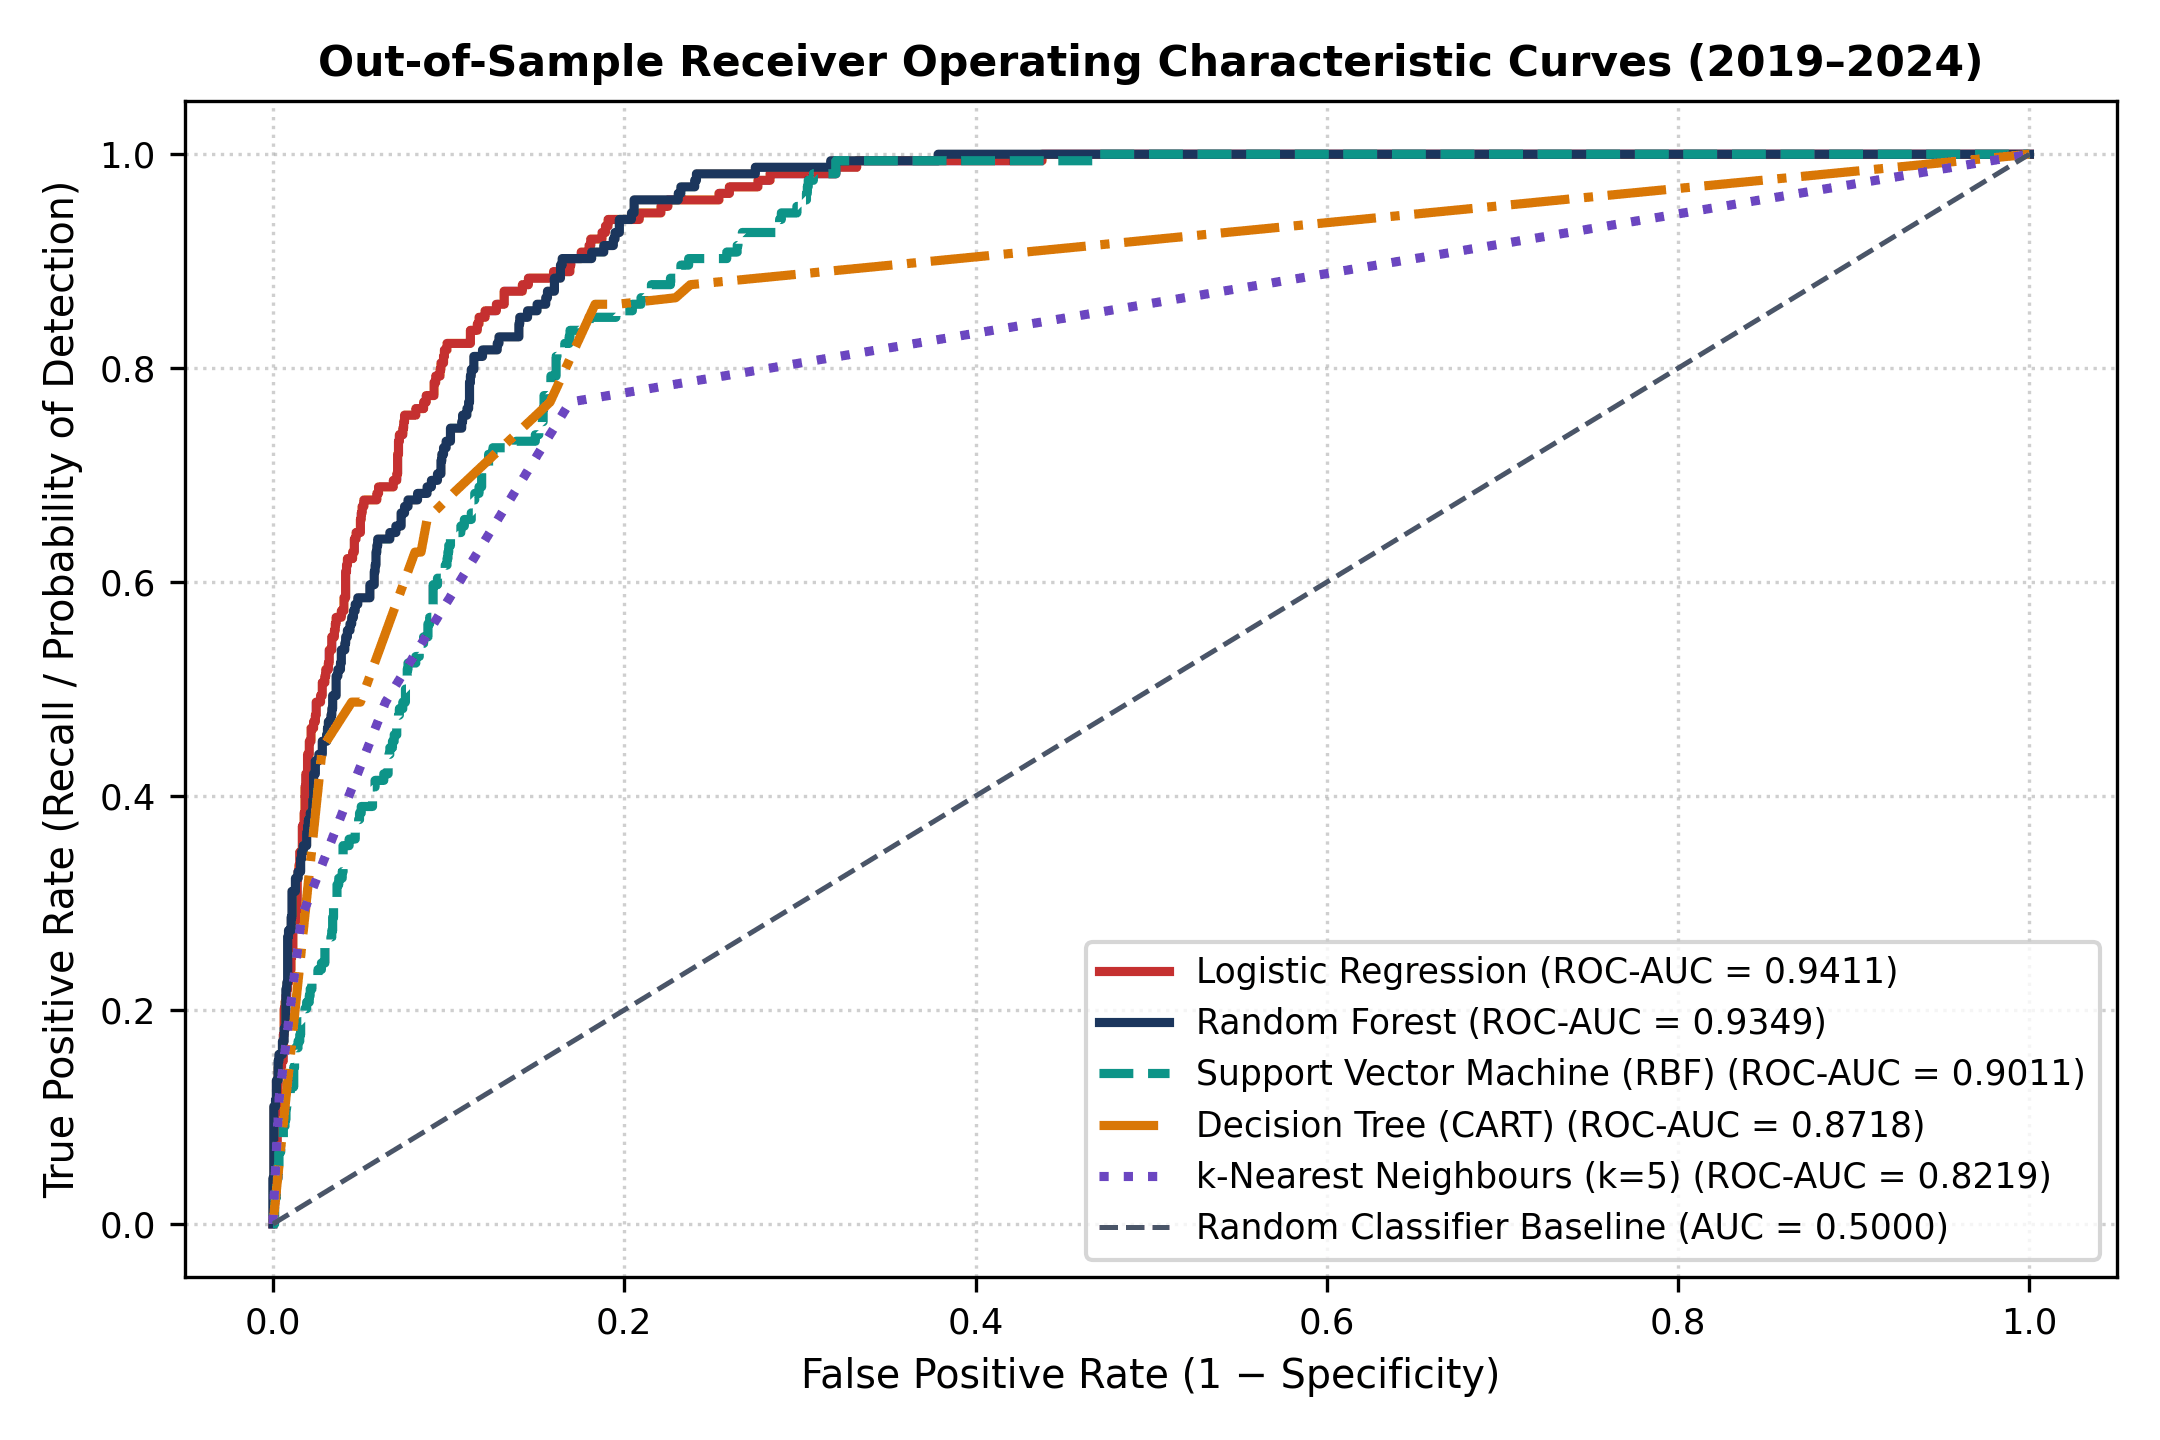
\includegraphics[width=\columnwidth]{figures/figure_07_roc_curves.png}
\caption{Receiver Operating Characteristic (ROC) curves across all five classifiers on the 2019--2024 holdout test set (2,192 days).}
\label{fig:f7}
\end{figure}

\begin{figure}[H]
\centering
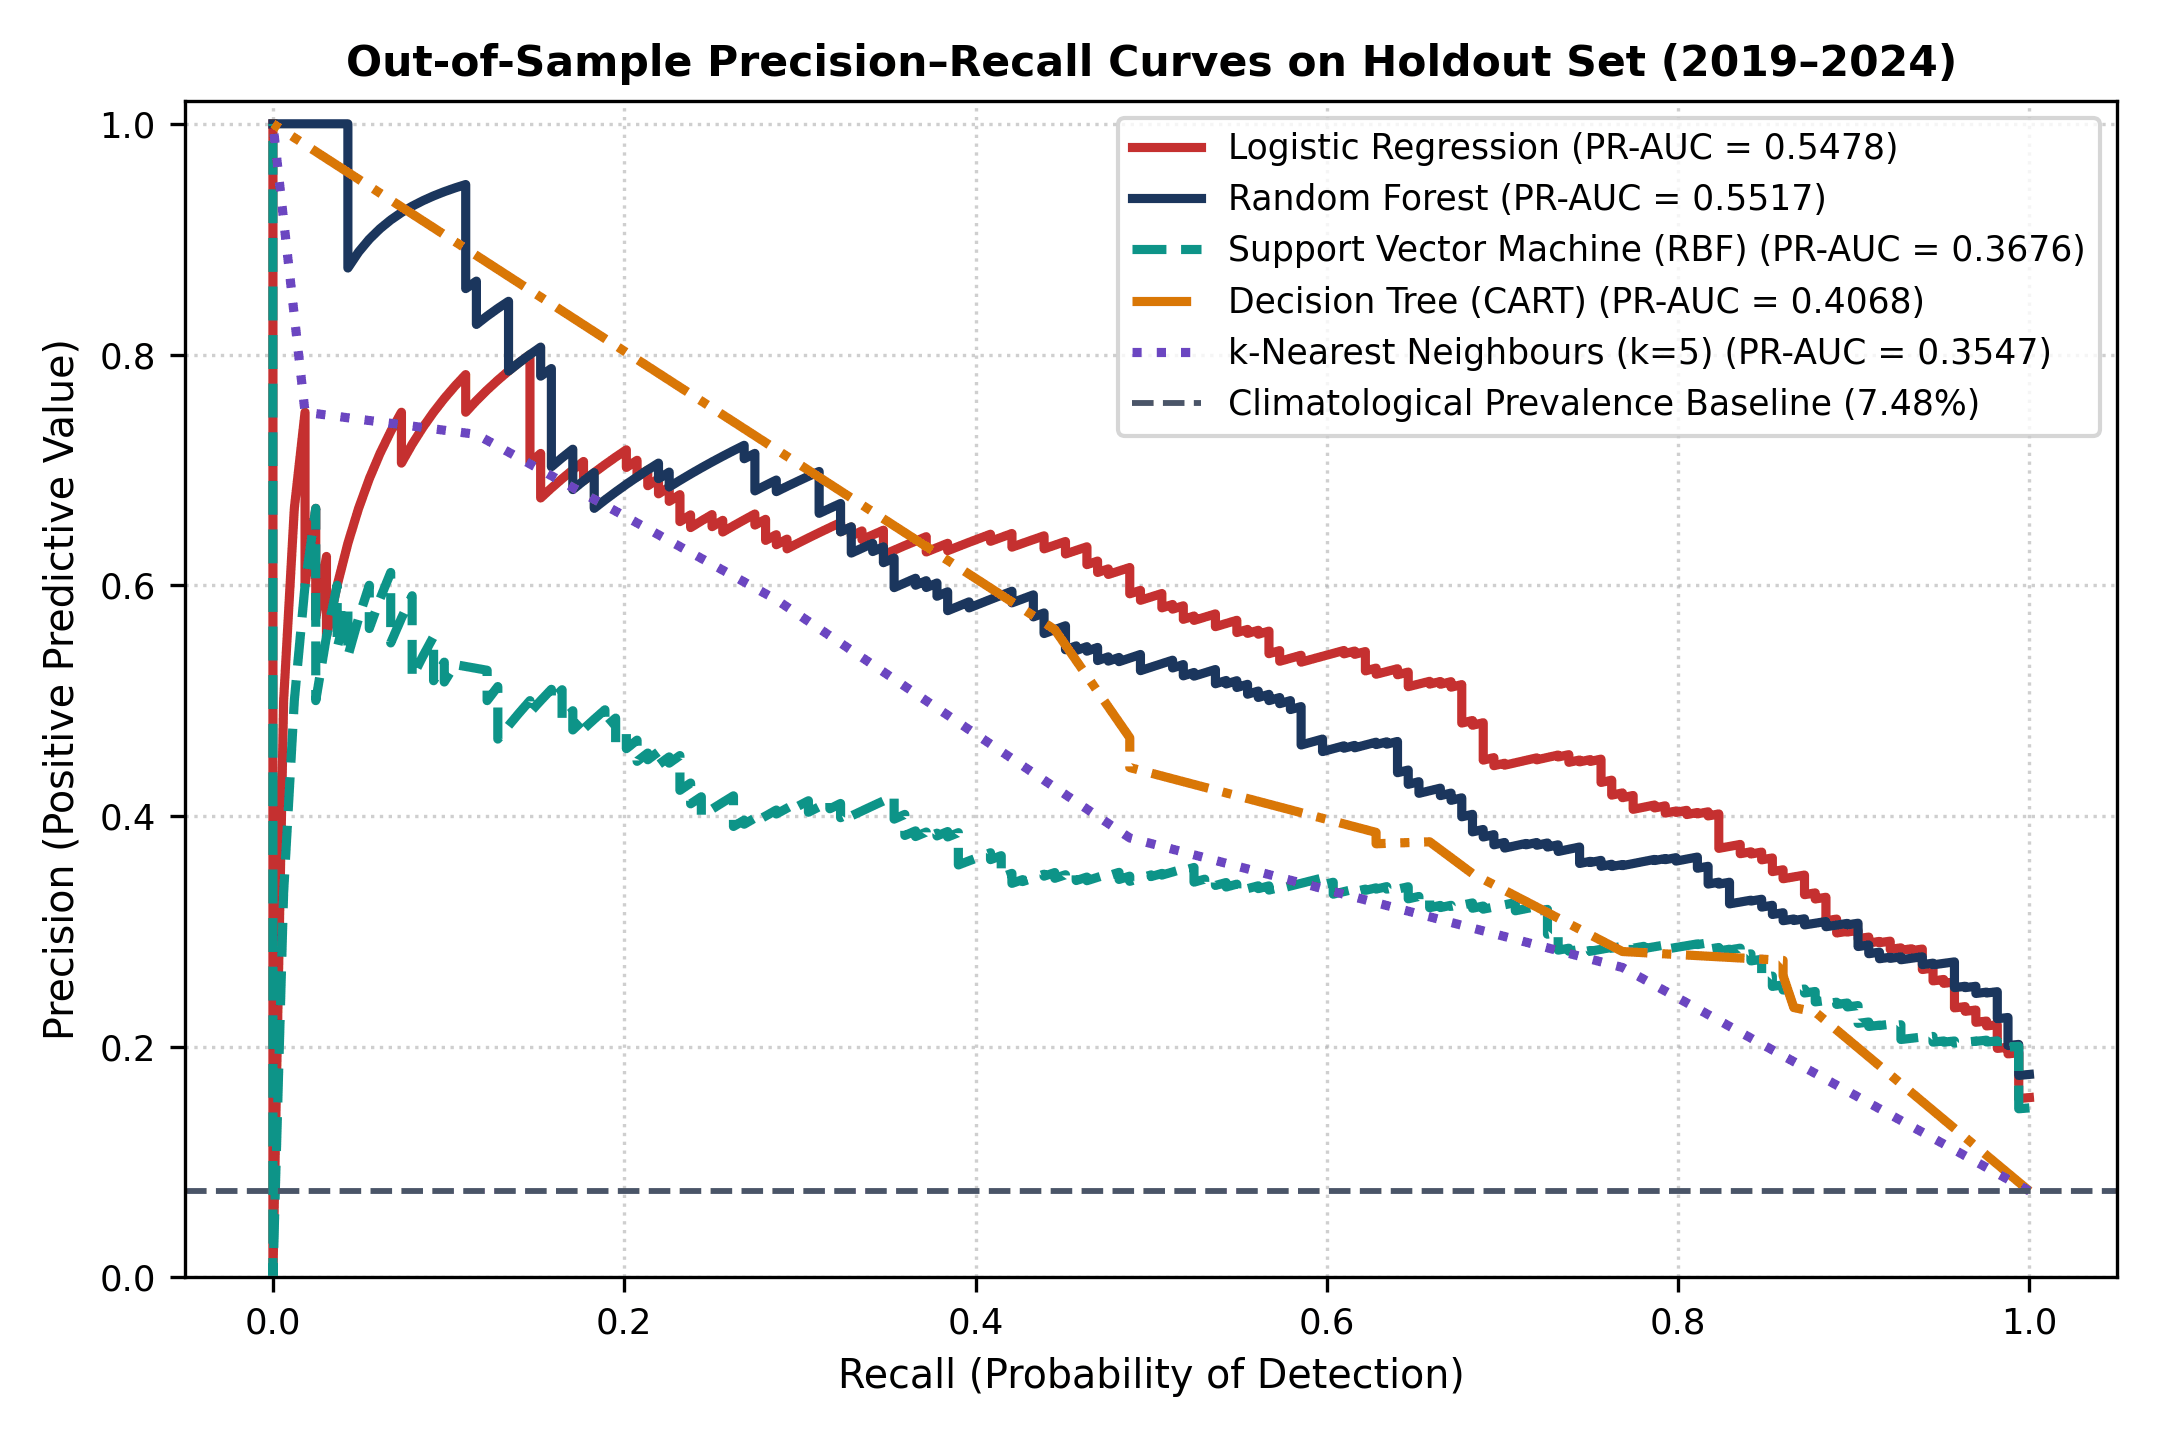
\includegraphics[width=\columnwidth]{figures/figure_08_pr_curves.png}
\caption{Precision-Recall curves on the 2019--2024 holdout test set against the 7.48\% storm prevalence baseline, showing Random Forest (0.5517) and Logistic Regression (0.5478) achieving over a seven-fold gain above random chance.}
\label{fig:f8}
\end{figure}

\begin{figure*}[!t]
\centering
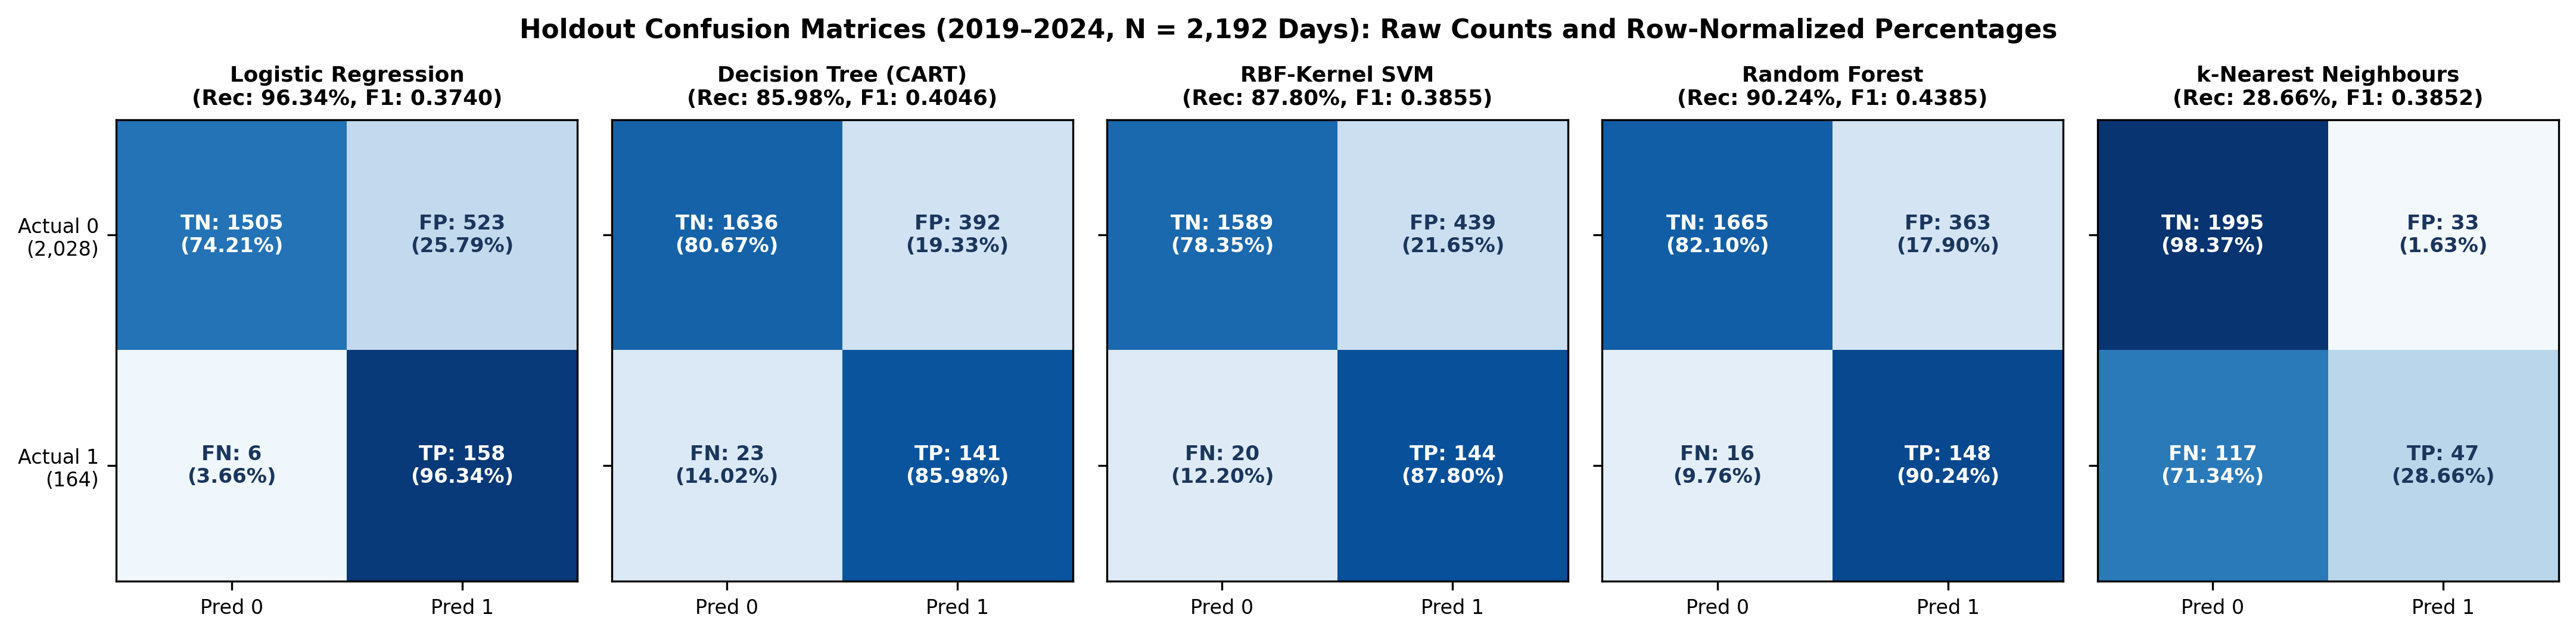
\includegraphics[width=0.95\textwidth]{figures/figure_09_confusion_matrices.png}
\caption{Holdout confusion matrices across all five classifiers (2019--2024, 2,192 days: 2,028 non-extreme, 164 extreme) showing raw counts and row percentages.}
\label{fig:f9}
\end{figure*}

\subsubsection{Random Forest: Best Overall Operational Balance}
Comparing the five models in Table~\ref{tab:t7} and Figs.~\ref{fig:f7}--\ref{fig:f9} shows that Random Forest records the highest holdout F1-score (0.4385, with a 95\% block-bootstrap confidence interval of 38.17\% to 49.14\%) and the highest Precision-Recall AUC (0.5517, more than 7.3 times higher than the 0.0748 no-skill baseline), alongside an ROC-AUC of 0.9349, 82.71\% accuracy, and 90.24\% recall (catching 148 of 164 extreme storms). Compared with a single Decision Tree (F1 of 0.4046, 23 missed storms, and 392 false alarms), combining 100 trees with random 4-feature splits catches 7 additional extreme storms while eliminating 29 false alarms.

\subsubsection{Logistic Regression: Maximum Storm Sensitivity}
Class-weighted Logistic Regression achieves the highest default-cutoff recall of 96.34\% (catching 158 of 164 extreme rain days and missing only 6 storms across 6 years) and the highest ROC-AUC (0.9411). However, because its straight-line boundary cannot bend around warm, humid monsoon break days, it produces 523 false alarms (160 more false alarms than Random Forest), resulting in 23.20\% precision and an F1-score of 0.3740.

\subsubsection{RBF-SVM: Strong Calibration but Lower Precision-Recall Skill}
RBF-SVM detects 144 of 164 storms (87.80\% recall, ROC-AUC of 0.9011) and achieves the lowest Brier calibration error (0.0553) thanks to internal Platt scaling, but its Precision-Recall AUC (0.3676) lags substantially behind Random Forest (0.5517) because of high-probability false alarms on humid days.

\subsubsection{k-Nearest Neighbours: Demonstration of the Accuracy Paradox}
Unweighted k-NN (5 neighbours) appears best if judged by overall accuracy (93.16\%) or precision (58.75\%), yet it misses 117 out of 164 extreme storms (28.66\% recall, catching only 47 events). Because 92.52\% of test days are non-extreme, a trivial model that predicts ``no extreme rain'' every single day achieves 92.52\% accuracy while catching zero floods.

\subsubsection{Feature Importance and Physical Drivers}
Table~\ref{tab:t8} and Fig.~\ref{fig:f10} compare how Random Forest, Decision Tree (CART), Logistic Regression, and test-set permutation importance rank the top 10 weather predictors. This comparison explains why Random Forest outperforms a single Decision Tree. When a single CART tree evaluates all 22 predictors greedily at every split, it assigns 73.35\% of its total decision weight to yesterday's rainfall (\texttt{precip\_lag1}) while giving 0.00\% weight to specific humidity (\texttt{QV2M}) and 7-day rainfall accumulation (\texttt{precip\_roll7}). In contrast, because Random Forest restricts each split to 4 randomly chosen predictors, it spreads decision weight across multi-day rainfall memory (\texttt{precip\_lag1} at 20.83\%, \texttt{precip\_roll3} at 11.55\%, and \texttt{precip\_roll7} at 5.24\%), atmospheric moisture (\texttt{QV2M} at 10.37\%, \texttt{T2MDEW} at 9.36\%, \texttt{RH2M} at 5.43\%, and \texttt{dew\_point\_depression} at 5.12\%), and cloud cooling (\texttt{temp\_diurnal\_range} at 7.00\% and \texttt{ALLSKY\_SW} at 4.41\%). Logistic Regression weights and permutation tests confirm the same physical mechanism: high previous-day rain and high relative humidity strongly increase storm probability, whereas bright sunshine and wide daily temperature ranges strongly indicate dry weather.

\begin{table}[H]
\caption{TOP-10 WEATHER PREDICTOR IMPORTANCE RANKINGS ACROSS MODELS}
\label{tab:t8}
\centering
\resizebox{\columnwidth}{!}{%
\begin{tabular}{clcccc}
\toprule
\textbf{Rank} & \textbf{Predictor Variable} & \textbf{Random Forest} & \textbf{Decision Tree} & \textbf{Logistic Reg. Weight} & \textbf{Permutation Drop} \\
\midrule
1 & precip\_lag1 (Yesterday rain) & \textbf{0.2083} & \textbf{0.7335} & \textbf{+0.4969} & \textbf{0.0721} \\
2 & precip\_roll3 (3-day rain) & 0.1155 & 0.0109 & +0.1092 & 0.0105 \\
3 & QV2M (Specific humidity) & 0.1037 & 0.0000 & +0.2888 & 0.0034 \\
4 & T2MDEW (Dew point) & 0.0936 & 0.0037 & +0.3057 & 0.0012 \\
5 & temp\_diurnal\_range & 0.0700 & 0.0461 & -0.4886 & 0.0099 \\
6 & RH2M (Relative humidity) & 0.0543 & 0.0122 & +0.4679 & 0.0070 \\
7 & precip\_roll7 (7-day rain) & 0.0524 & 0.0000 & +0.0756 & 0.0018 \\
8 & dew\_point\_depression & 0.0512 & 0.0086 & -0.3168 & 0.0039 \\
9 & ALLSKY\_SW (Solar radiation) & 0.0441 & 0.0322 & \textbf{-0.5355} & 0.0206 \\
10 & T2M\_MIN (Min temperature) & 0.0349 & 0.0097 & +0.2000 & 0.0005 \\
\bottomrule
\end{tabular}%
}
\end{table}

\begin{figure}[H]
\centering
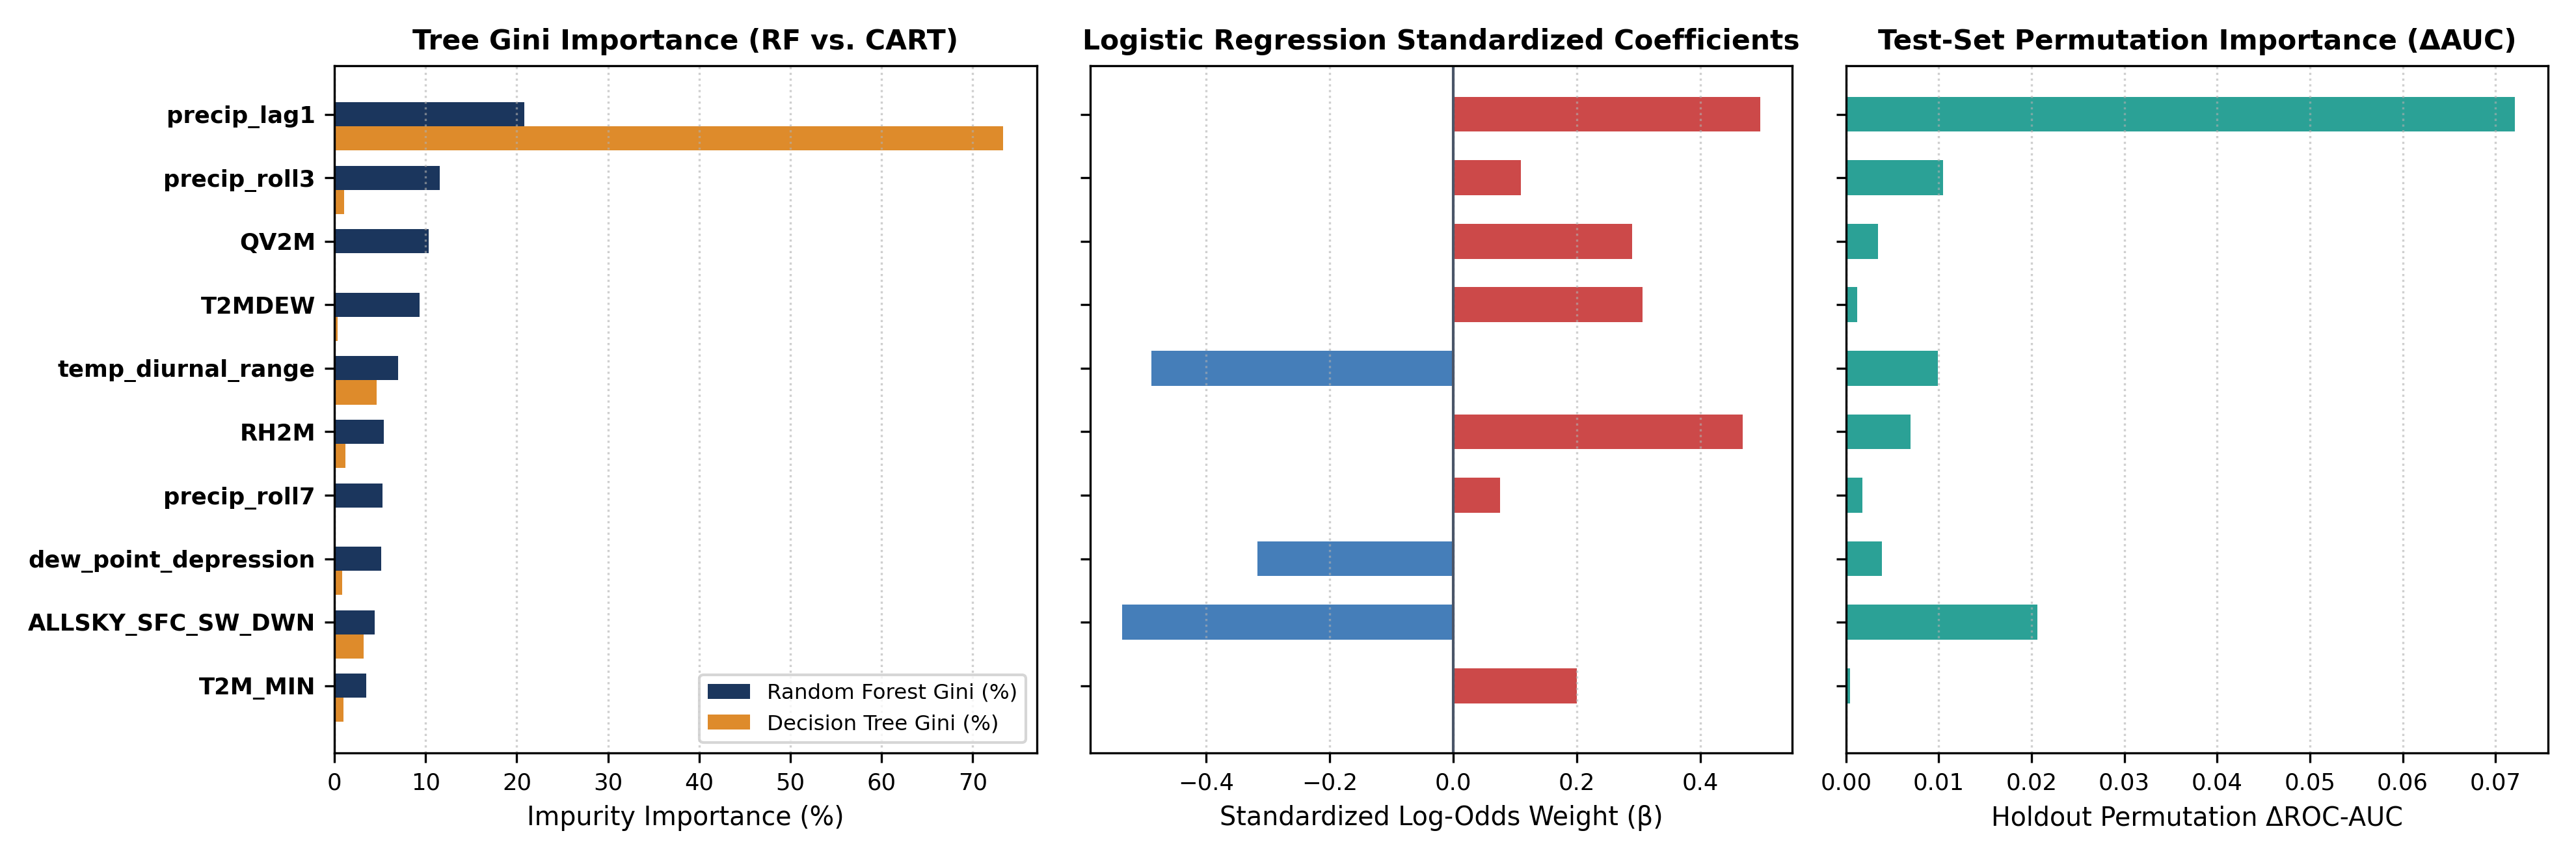
\includegraphics[width=\columnwidth]{figures/figure_10_feature_attribution.png}
\caption{Comparison of top-10 weather predictors: Random Forest versus Decision Tree Gini importance (left), Logistic Regression standardized weights (centre), and holdout test permutation importance (right).}
\label{fig:f10}
\end{figure}

\subsubsection{Probability Calibration and Subspace Ablation}
Fig.~\ref{fig:f11} compares the probability calibration curves and Brier scores across all five models. Platt-scaled RBF-SVM (0.0553) and unweighted k-NN (0.0560) record the lowest raw Brier scores because their predicted probabilities stay close to the 7.48\% average storm rate, whereas balanced class weighting in Random Forest (0.1154), CART (0.1418), and Logistic Regression (0.1621) intentionally pushes storm probabilities upward to prevent missed floods. Table~\ref{tab:t9} reports paired McNemar statistical comparisons alongside the PCA dimensionality reduction ablation test. Part A confirms that Random Forest catches 101 extreme storms missed by k-NN while k-NN catches zero storms missed by Random Forest (highly significant with $p < 10^{-30}$). Part B shows that replacing the 22 physical features with the 7 PCA components reduces Logistic Regression recall from 96.34\% to 93.29\% (F1 dropping from 0.3740 to 0.3562) and reduces k-NN recall from 28.66\% to 24.39\% (F1 dropping from 0.3852 to 0.3265), confirming that retaining all 22 physical predictors preserves vital storm precursors.

\begin{figure}[H]
\centering
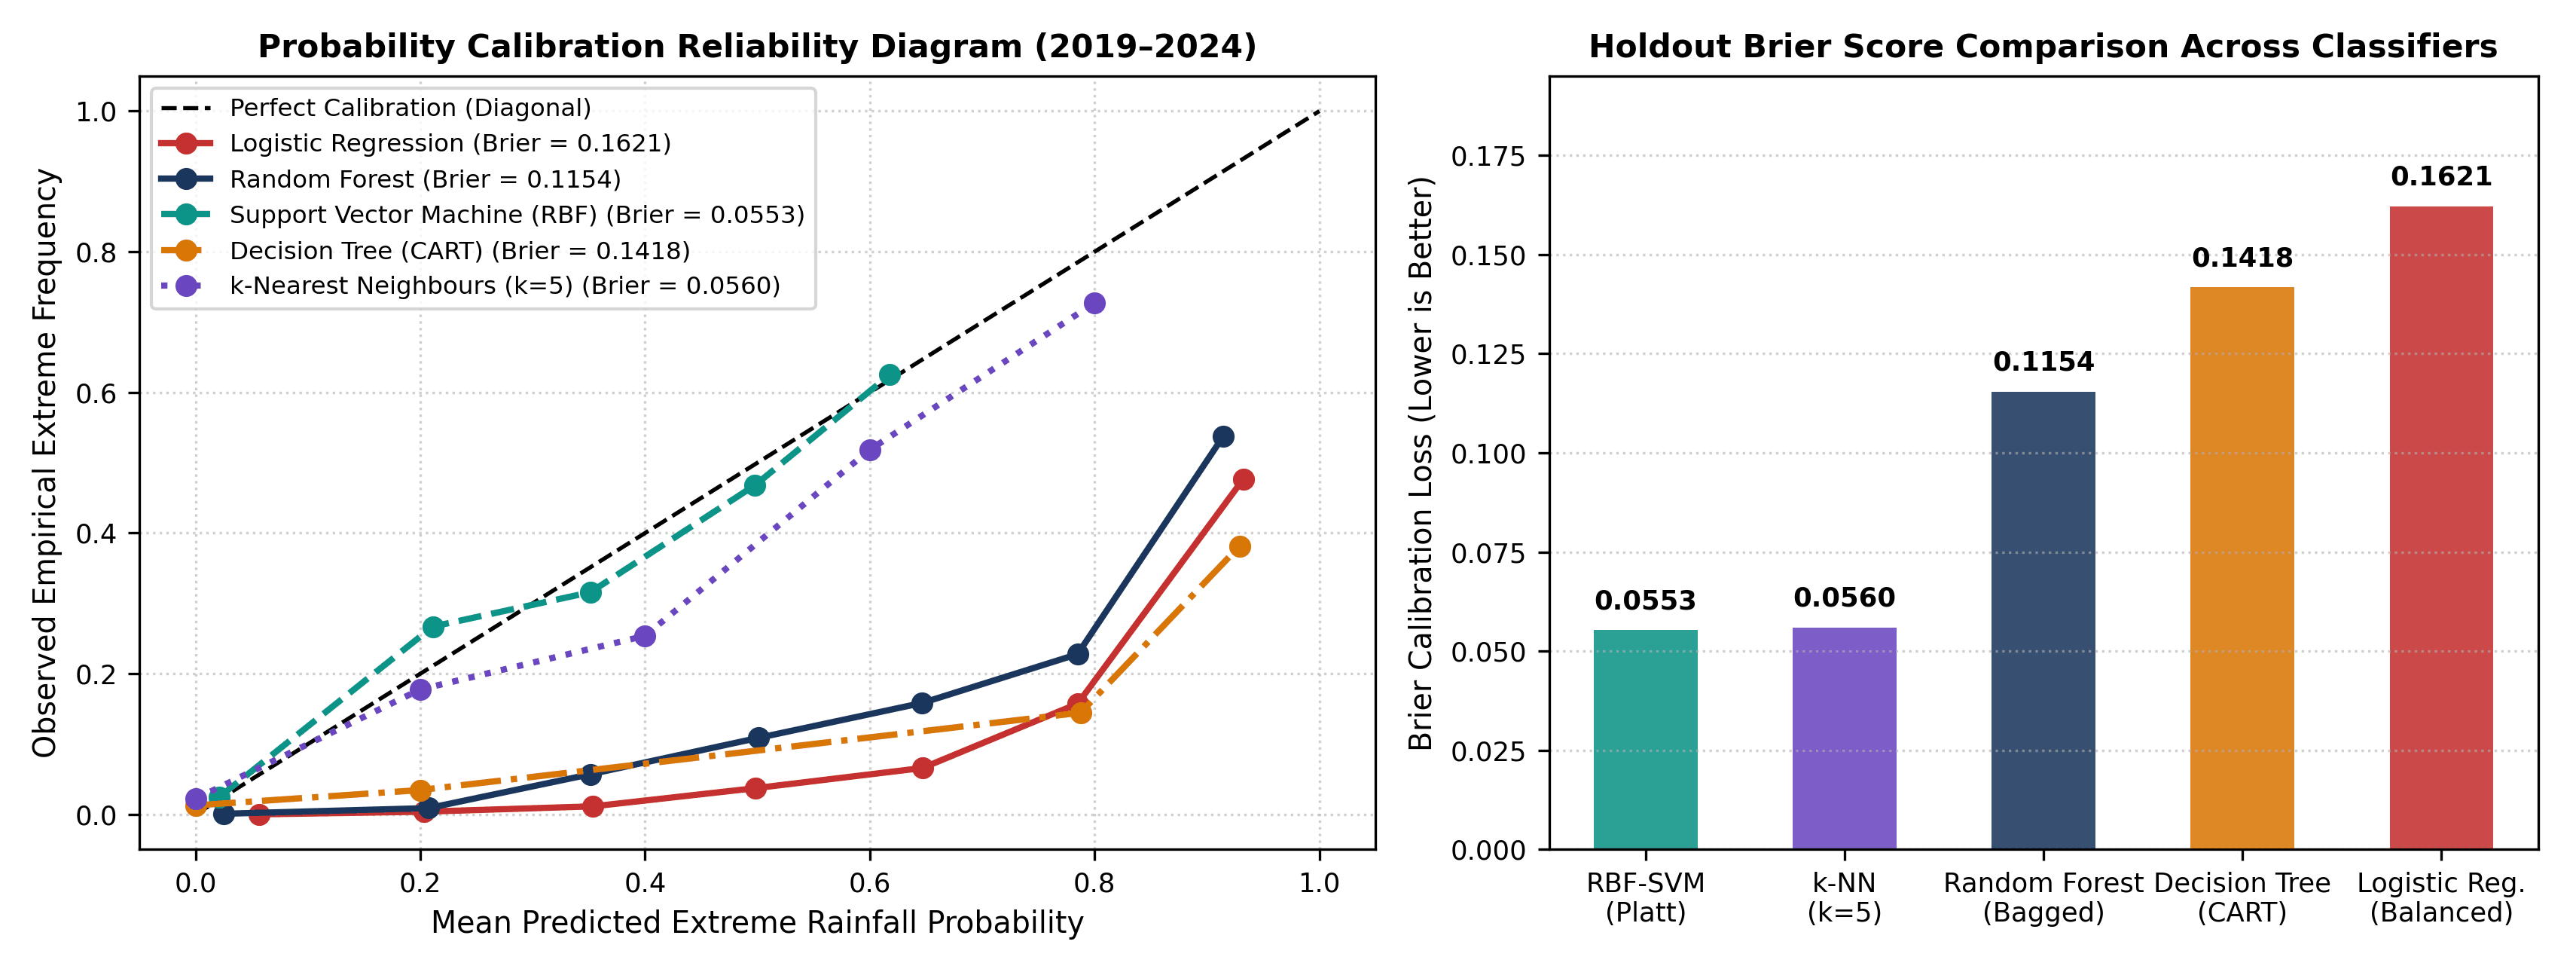
\includegraphics[width=\columnwidth]{figures/figure_11_calibration_reliability.png}
\caption{Probability calibration curves across all five classifiers on the 2019--2024 holdout test set (left) and Brier score comparison showing the effect of balanced class weighting versus Platt scaling (right).}
\label{fig:f11}
\end{figure}

\begin{table}[H]
\caption{PAIRED MCNEMAR SIGNIFICANCE TESTS AND 7-COMPONENT PCA VERSUS 22-FEATURE ABLATION (2019--2024 TEST SET)}
\label{tab:t9}
\centering
\resizebox{\columnwidth}{!}{%
\begin{tabular}{lcccc}
\toprule
\textbf{Part A: Paired Model Comparison} & \textbf{All Days Disagreed} & \textbf{Chi-Square (p-value)} & \textbf{Storms Disagreed} & \textbf{Storm Chi-Square (p)} \\
\midrule
Random Forest vs. k-NN & 106 vs. 335 & 117.88 ($< 10^{-28}$) & \textbf{101 vs. 0} & \textbf{99.01 ($< 10^{-30}$)} \\
Logistic Regression vs. k-NN & 112 vs. 491 & 236.96 ($< 10^{-56}$) & \textbf{111 vs. 0} & \textbf{109.01 ($< 10^{-33}$)} \\
Random Forest vs. Decision Tree & 99 vs. 63 & 7.56 (0.0058) & 13 vs. 6 & 1.89 (0.170) \\
Random Forest vs. RBF-SVM & 135 vs. 55 & 32.85 ($< 10^{-8}$) & 13 vs. 9 & 0.41 (0.520) \\
Logistic Reg. vs. Random Forest & 22 vs. 172 & 114.44 ($< 10^{-29}$) & 11 vs. 1 & 6.75 (0.0063) \\
\midrule
\textbf{Part B: PCA Subspace Ablation} & \textbf{Accuracy (\%)} & \textbf{Storm Recall (\%)} & \textbf{F1-Score} & \textbf{ROC / PR-AUC} \\
\midrule
Logistic Reg. (Full 22 Features) & \textbf{75.87} & \textbf{96.34} & \textbf{0.3740} & \textbf{0.9411 / 0.5478} \\
Logistic Reg. (7 PCA Modes, 91.5\%) & 74.77 & 93.29 & 0.3562 & 0.9287 / 0.5240 \\
k-NN (Full 22 Features) & \textbf{93.16} & \textbf{28.66} & \textbf{0.3852} & \textbf{0.8219 / 0.3547} \\
k-NN (7 PCA Modes, 91.5\%) & 92.47 & 24.39 & 0.3265 & 0.8159 / 0.3053 \\
\bottomrule
\end{tabular}%
}
\end{table}

\subsection{Operational and Flood Case Study Results (RO3)}

\subsubsection{Cost-Sensitive Threshold Optimisation}
Table~\ref{tab:t10} and Fig.~\ref{fig:f12} evaluate how adjusting the Random Forest warning threshold changes storm detection and total disaster cost under the 15-to-1 penalty rule (where each missed storm costs 15 points and each false alarm costs 1 point). At the standard 0.50 cutoff, Random Forest misses 16 extreme storms and produces 363 false alarms, resulting in a total 15-to-1 cost of 603. When we apply the \textbf{leak-free training cross-validation threshold} of 0.30 (chosen strictly using 1995--2018 training folds without viewing test data), holdout storm recall rises from 90.24\% to \textbf{near-complete storm detection} (98.17\% recall, catching 161 of 164 extreme rain events), cutting missed storms by more than 81\% (from 16 down to just 3 missed storms) and lowering total disaster cost from 603 to 550. For comparison, the post-hoc test minimum occurs at a threshold of 0.40 (catching 157 of 164 storms with a cost of 532), which is reported only as a retrospective reference because finding it requires looking at test labels.

\begin{table}[H]
\caption{RANDOM FOREST COST-SENSITIVE THRESHOLD SWEEP UNDER THE 15-TO-1 MISSED-STORM PENALTY (2019--2024 TEST SET)}
\label{tab:t10}
\centering
\resizebox{\columnwidth}{!}{%
\begin{tabular}{lccccccc}
\toprule
\textbf{Probability Cutoff \& Rule} & \textbf{Acc (\%)} & \textbf{Prec (\%)} & \textbf{Recall (\%)} & \textbf{F1} & \textbf{Caught / Missed} & \textbf{False Alarms} & \textbf{15:1 Cost} \\
\midrule
0.10 (High Standby Watch) & 61.59 & 16.30 & 100.00 & 0.2803 & 164 / 0 & 842 & 842 \\
0.20 (Low Warning Cutoff) & 70.44 & 20.12 & 99.39 & 0.3347 & 163 / 1 & 647 & 662 \\
\textbf{0.30 (Prospective Training CV)} & \textbf{76.82} & \textbf{24.17} & \textbf{98.17} & \textbf{0.3880} & \textbf{161 / 3} & \textbf{505} & \textbf{550 (OOF)} \\
0.35 (Intermediate Cutoff) & 78.38 & 25.16 & 95.73 & 0.3985 & 157 / 7 & 467 & 572 \\
\textit{0.40 (Retrospective Test Min)} & 80.20 & 26.88 & 95.73 & 0.4198 & 157 / 7 & 427 & 532 (Test) \\
0.50 (Standard Default Cutoff) & 82.71 & 28.96 & 90.24 & 0.4385 & 148 / 16 & 363 & 603 \\
0.60 (Moderate Confidence) & 84.72 & 31.13 & 85.98 & 0.4571 & 141 / 23 & 312 & 657 \\
0.70 (High-Priority Red Alert) & 87.96 & 36.19 & 79.88 & \textbf{0.4981} & 131 / 33 & 231 & 726 \\
\bottomrule
\end{tabular}%
}
\end{table}

\begin{figure}[H]
\centering
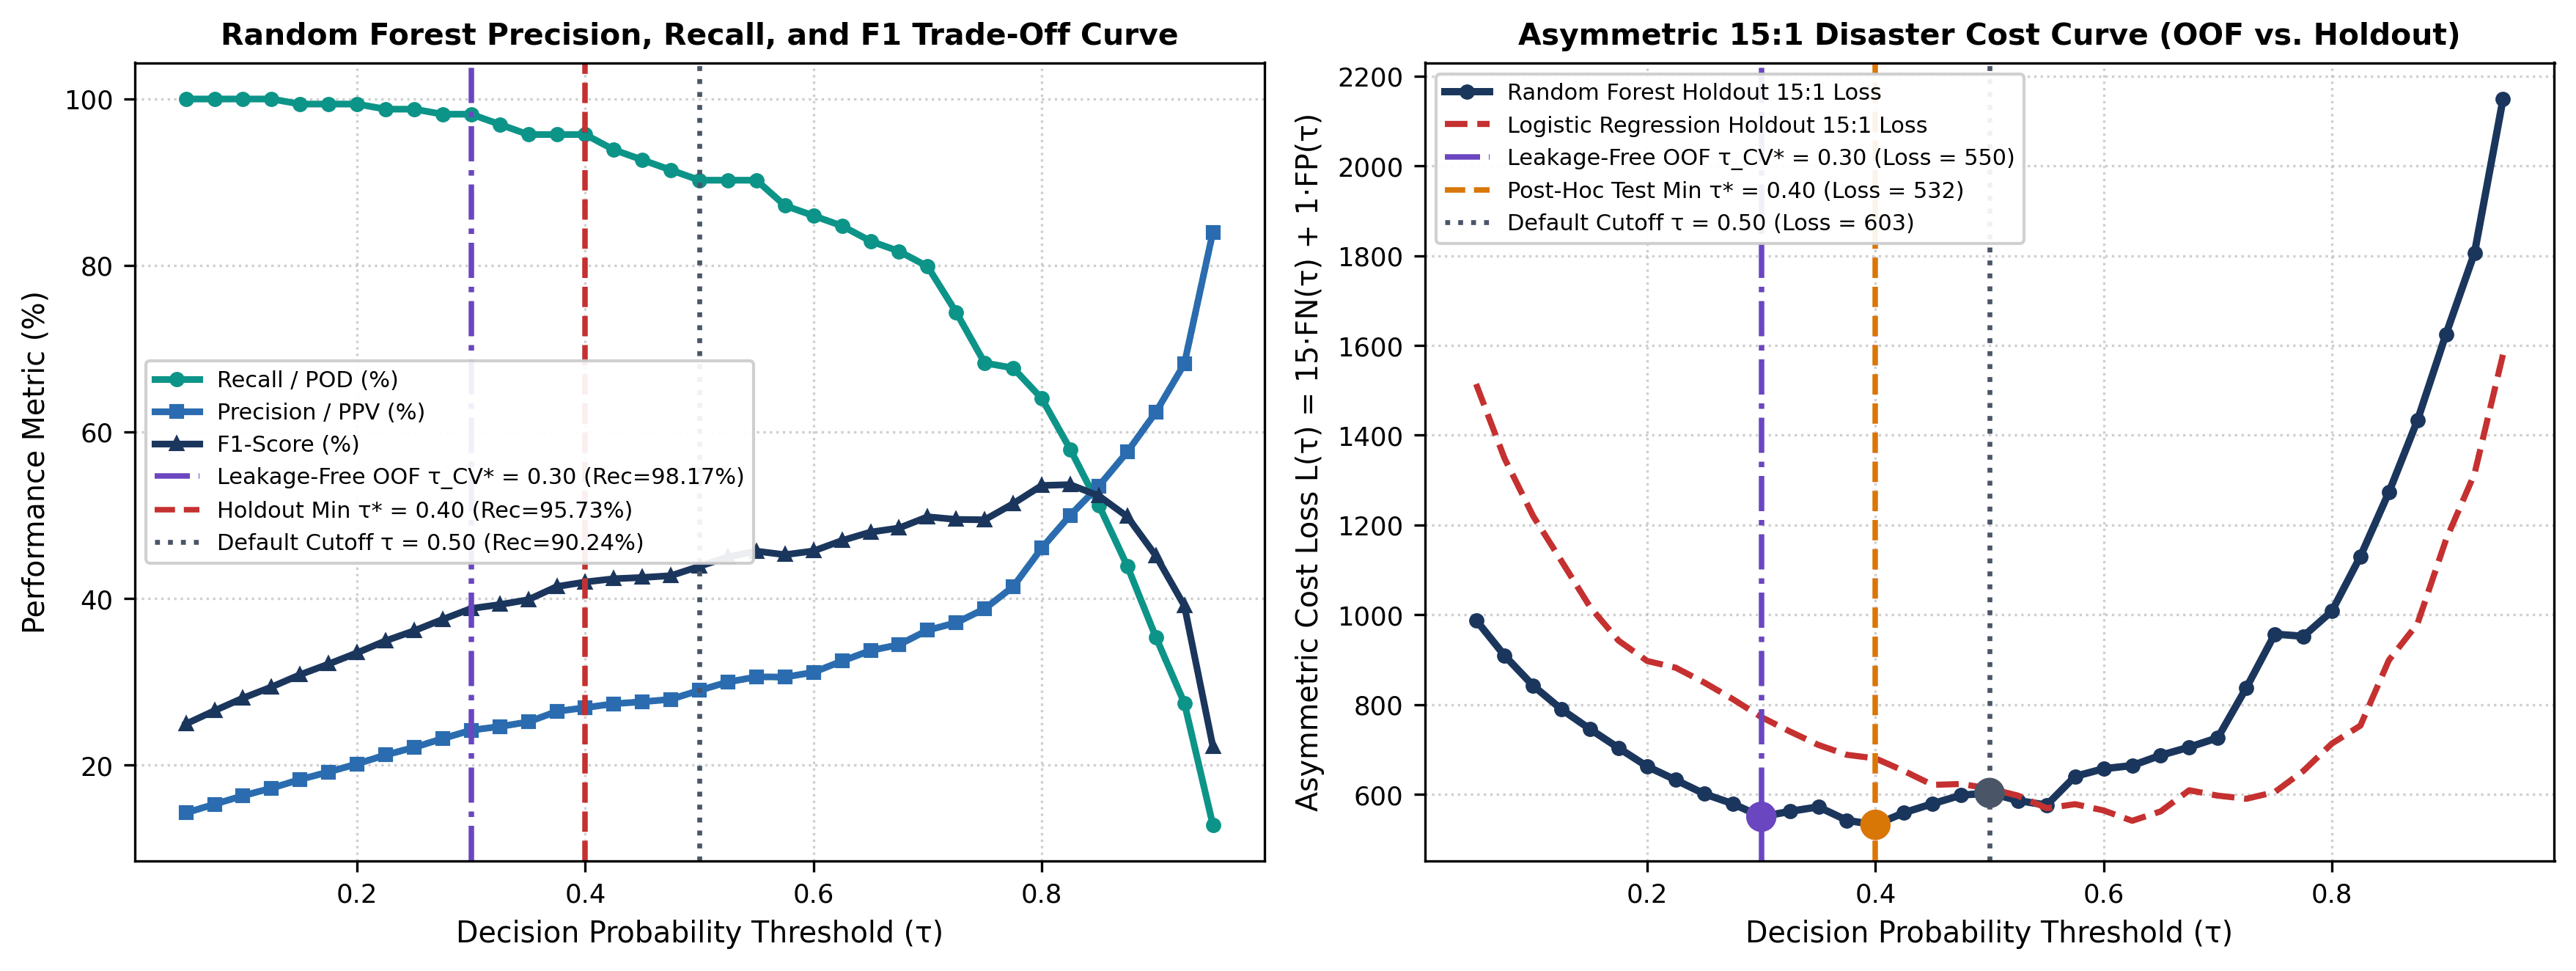
\includegraphics[width=\columnwidth]{figures/figure_12_threshold_cost_sweep.png}
\caption{Random Forest precision, recall, and F1 trade-off curves across probability cutoffs (left) and the 15-to-1 disaster cost curve comparing the training-derived 0.30 threshold against the 0.40 test minimum and 0.50 default cutoff (right).}
\label{fig:f12}
\end{figure}

\subsubsection{Retrospective Validation on the September 2024 Flood}
Fig.~\ref{fig:f13} tracks daily rainfall and model warning probabilities day by day across the catastrophic 20--30 September 2024 Kathmandu flood event \cite{ref6,ref7}. Following four days of light rain (0.39 to 1.14 mm/day during 20--23 September, where Random Forest probabilities remained low at 0.1831 or less), rainfall jumped suddenly to 47.54 mm/day on 24 September, 55.89 mm/day on 25 September, 16.56 mm/day on 26 September, 76.28 mm/day on 27 September, and 93.26 mm/day on 28 September. On the sudden first-day onset (24 September, when yesterday's rain was only 0.58 mm), same-day Logistic Regression immediately detected the spike in relative humidity (90.47\%) and cloud cooling (daily temperature range compressed to 3.66$^\circ$C), issuing a strong warning probability of 0.7154. From 25 to 28 September, once 1-day and 3-day rain memory engaged, both Random Forest (probabilities of 0.7189, 0.6992, 0.6973, and 0.6881) and Logistic Regression (probabilities of 0.9962, 0.9939, 0.8674, and 0.9997) issued sustained high-confidence flood alerts well above both the 0.30 and 0.50 thresholds.

\begin{figure}[H]
\centering
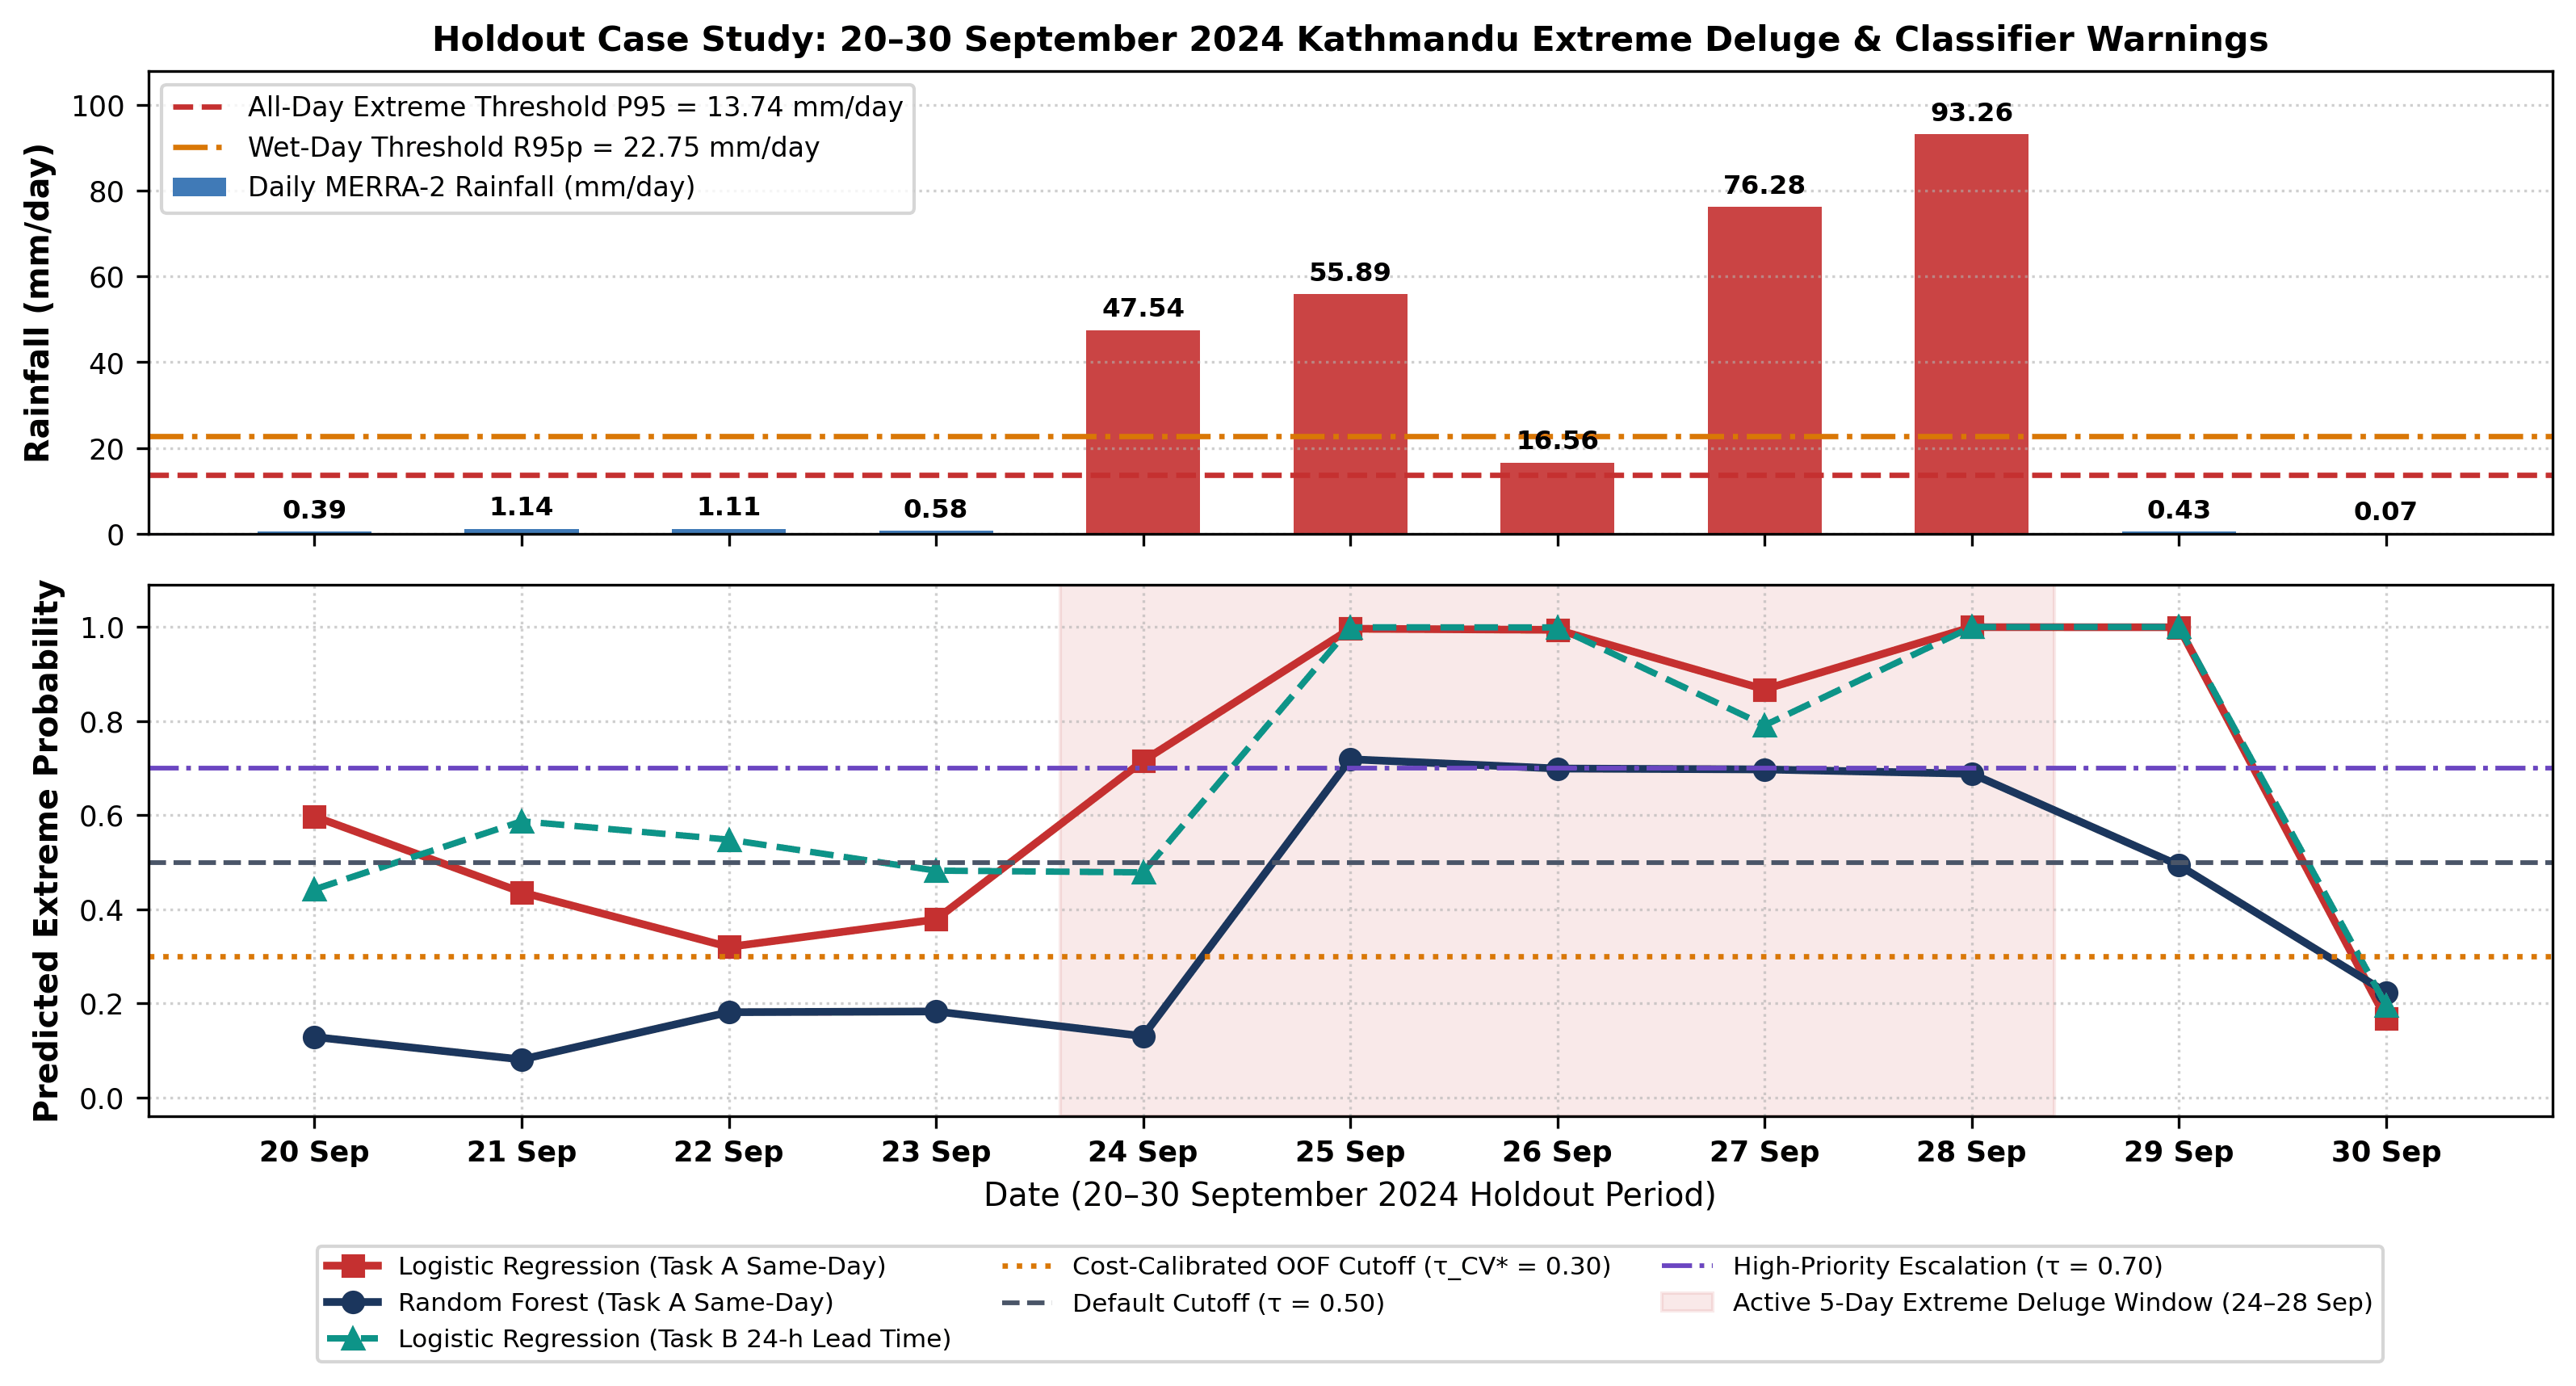
\includegraphics[width=\columnwidth]{figures/figure_13_sept2024_case_study.png}
\caption{Retrospective timeline of the 20--30 September 2024 Kathmandu flood disaster: daily rainfall against the 13.74 mm/day and 22.75 mm/day thresholds (top), and predicted storm probabilities from Random Forest and Logistic Regression (bottom).}
\label{fig:f13}
\end{figure}

\subsubsection{24-Hour Advance Forecasting and Wet-Day Benchmarks}
Table~\ref{tab:t11} and Fig.~\ref{fig:f14} compare model performance across Task A (same-day atmospheric state classification), Task B (strict 24-hour advance forecasting where all weather predictors come from yesterday or earlier), and Task C (severe wet-day deluge classification above 22.75 mm/day). Under the strict 24-hour lead time (Task B), Random Forest maintains the highest balanced F1-score (0.4097), catching 144 of 164 extreme storms a full day in advance (87.80\% recall, ROC-AUC of 0.9135, Precision-Recall AUC of 0.4194), while Logistic Regression catches 152 of 164 storms 24 hours ahead (92.68\% recall, ROC-AUC of 0.9088, Precision-Recall AUC of 0.4526). In contrast, k-NN recall drops to just 17.68\% on Task B (missing 135 of 164 storms). On Task C (wet-day threshold of 22.75 mm/day across 64 test deluges), Logistic Regression detects 62 of 64 severe deluges (96.88\% recall, ROC-AUC of 0.9461) and Random Forest detects 57 of 64 (89.06\% recall, ROC-AUC of 0.9276), confirming robust early-warning skill across both lead times and severity thresholds.

\begin{table}[H]
\caption{COMPARISON OF SAME-DAY CLASSIFICATION (TASK A), STRICT 24-HOUR ADVANCE FORECASTING (TASK B), AND WET-DAY DELUGE DETECTION (TASK C)}
\label{tab:t11}
\centering
\resizebox{\columnwidth}{!}{%
\begin{tabular}{lccccccc}
\toprule
\textbf{Forecasting Task \& Model} & \textbf{Acc (\%)} & \textbf{Prec (\%)} & \textbf{Recall (\%)} & \textbf{F1} & \textbf{ROC-AUC} & \textbf{PR-AUC} & \textbf{TP / FN / FP} \\
\midrule
\textbf{Task A (Same-Day, 13.74 mm)} -- RF & 82.71 & 28.96 & 90.24 & \textbf{0.4385} & 0.9349 & \textbf{0.5517} & 148 / 16 / 363 \\
\textbf{Task A (Same-Day, 13.74 mm)} -- LR & 75.87 & 23.20 & \textbf{96.34} & 0.3740 & \textbf{0.9411} & 0.5478 & 158 / 6 / 523 \\
\textbf{Task B (24-Hr Lead, 13.74 mm)} -- RF & 81.07 & 26.72 & 87.80 & \textbf{0.4097} & \textbf{0.9135} & 0.4194 & 144 / 20 / 395 \\
\textbf{Task B (24-Hr Lead, 13.74 mm)} -- LR & 72.31 & 20.35 & \textbf{92.68} & 0.3337 & 0.9088 & \textbf{0.4526} & 152 / 12 / 595 \\
\textbf{Task B (24-Hr Lead, 13.74 mm)} -- k-NN & \textbf{92.29} & \textbf{46.03} & 17.68 & 0.2555 & 0.7812 & 0.2509 & 29 / 135 / 34 \\
\textbf{Task C (Wet-Day, 22.75 mm)} -- RF & 83.85 & 14.11 & 89.06 & \textbf{0.2436} & 0.9276 & 0.2851 & 57 / 7 / 347 \\
\textbf{Task C (Wet-Day, 22.75 mm)} -- LR & 78.01 & 11.44 & \textbf{96.88} & 0.2046 & \textbf{0.9461} & \textbf{0.3985} & 62 / 2 / 480 \\
\bottomrule
\end{tabular}%
}
\end{table}

\begin{figure}[H]
\centering
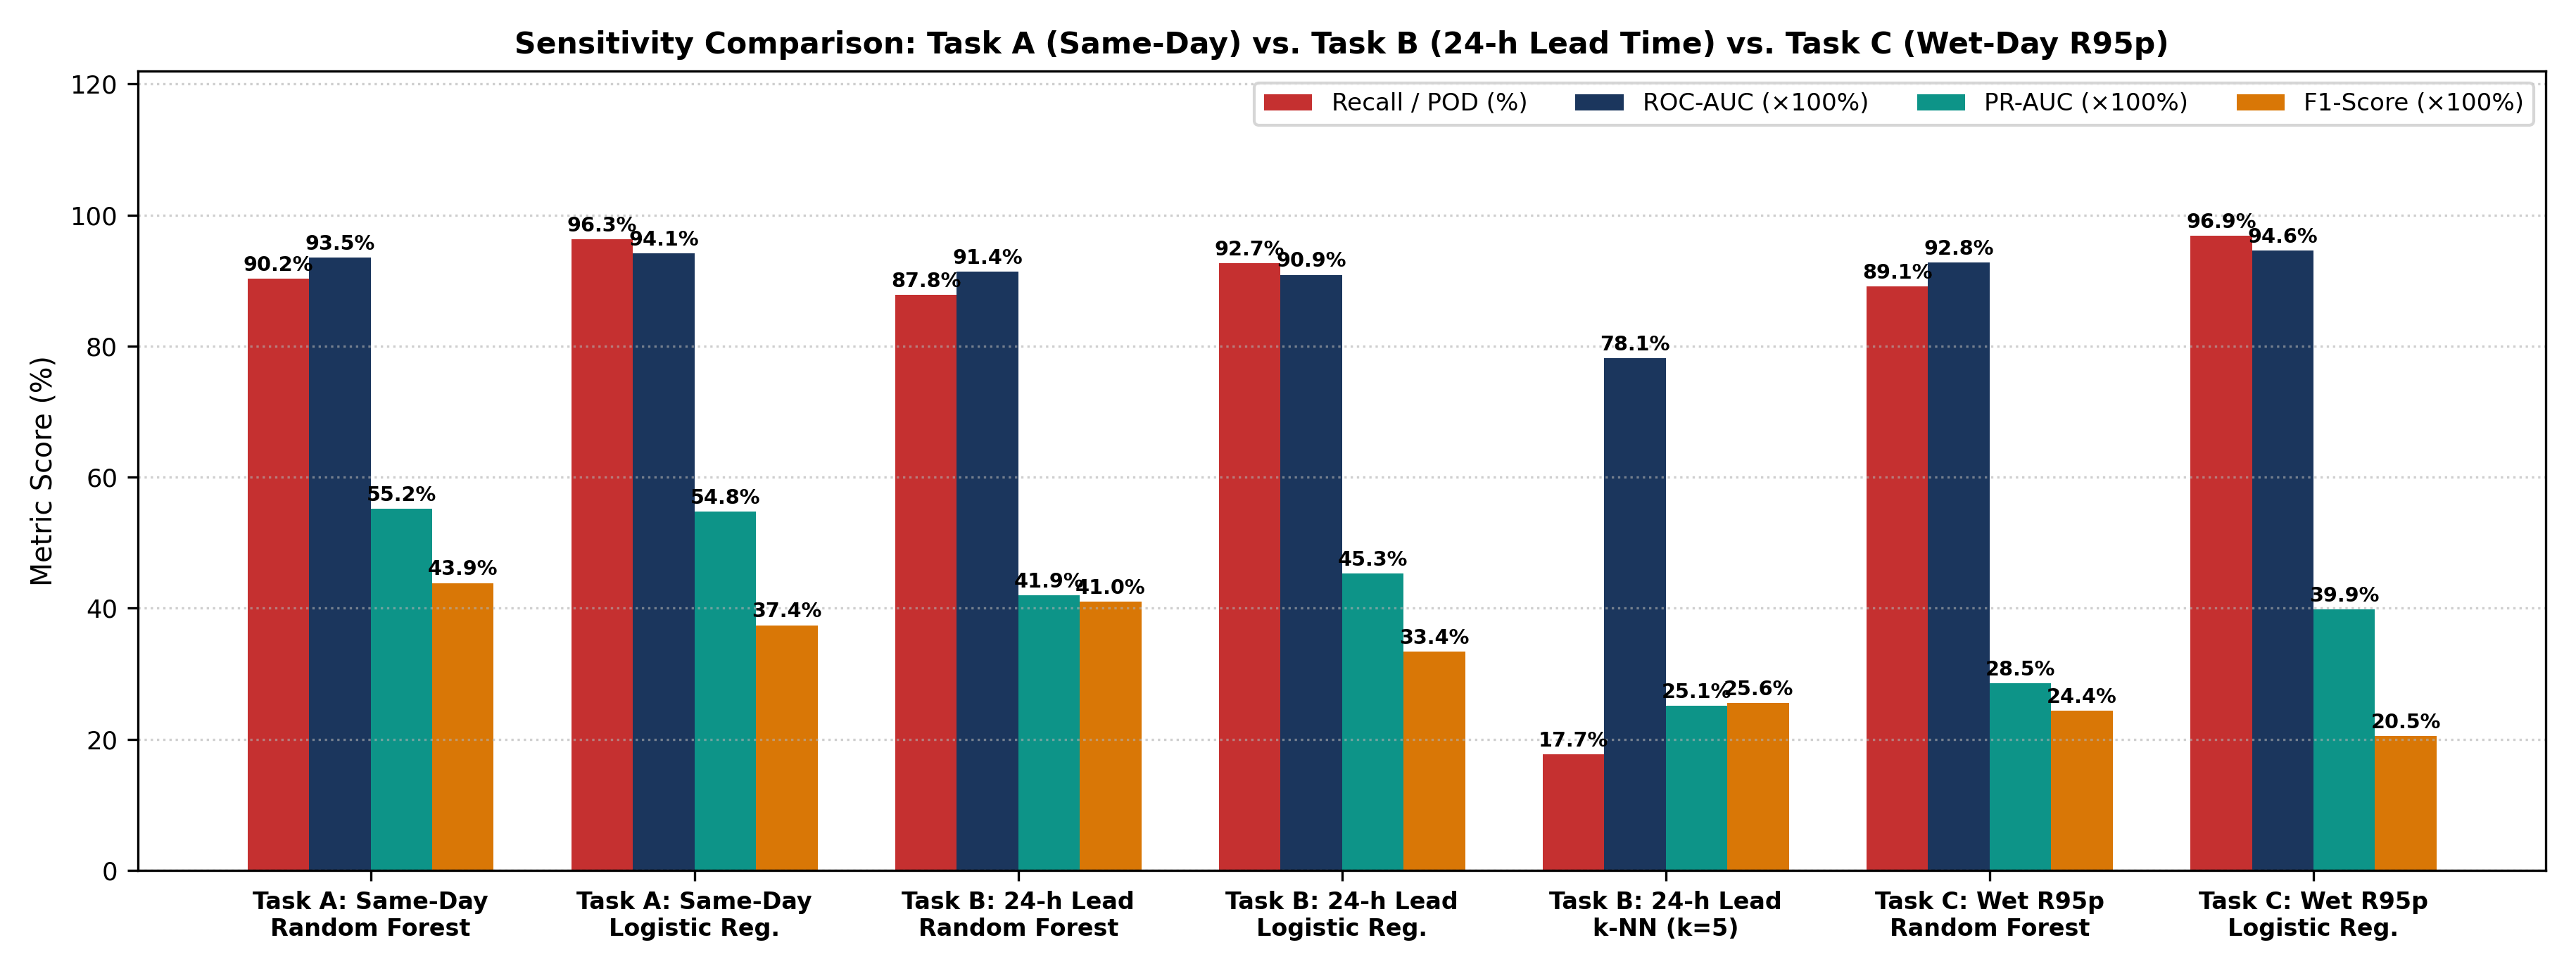
\includegraphics[width=\columnwidth]{figures/figure_14_lead_time_wetday_sensitivity.png}
\caption{Holdout performance comparison across Task A (same-day classification at 13.74 mm/day), Task B (strict 24-hour advance forecasting), and Task C (severe wet-day classification at 22.75 mm/day).}
\label{fig:f14}
\end{figure}

\subsubsection{Practical Comparison Across All Three Operational Tasks}
Comparing Tasks A, B, and C side by side demonstrates that model rankings remain consistent across different warning horizons and rainfall thresholds. Across every task, Random Forest and Logistic Regression form the top-performing pair, whereas unweighted k-NN consistently ranks last in storm detection. Moving from same-day diagnosis (Task A) to 24-hour advance forecasting (Task B) lowers Random Forest recall by only 2.44 percentage points (from 90.24\% to 87.80\%, or 4 additional missed storms over 6 years) and lowers Logistic Regression recall by only 3.66 percentage points (from 96.34\% to 92.68\%). This small drop confirms that multi-day valley moisture build-up and 3-to-7-day past rainfall totals carry strong predictive memory a full day before heavy rain arrives.

\section{Discussion and Conclusions}

\subsection{Why PCA Hurts Recall and Why k-NN Fails}

\subsubsection{Effect of PCA Compression on Storm Signals}
A key finding linking RO1 and RO2 is that while PCA compresses the 22 weather predictors into 7 components capturing 91.46\% of overall variance, training supervised models on those 7 components reduces storm recall by 3.05 percentage points for Logistic Regression and 4.27 percentage points for k-NN (Table~\ref{tab:t9}). The practical reason is straightforward: PCA ranks components by day-to-day seasonal variation across the entire year (which is dominated by the smooth shift between dry winters and warm summers) rather than rare one-day storm spikes. Blending all 22 variables into 7 combined axes blurs sharp single-variable warning signs---such as a sudden jump in yesterday's rainfall or a sharp drop in daily temperature range---that classifiers rely on to spot extreme cloudbursts \cite{ref16,ref17}.

\subsubsection{Why Unweighted k-NN Suffers the Accuracy Paradox}
Comparing the five classifiers refutes claims in earlier urban rainfall studies \cite{ref2} that unweighted k-NN is suitable for rainfall prediction. On the 2019--2024 Kathmandu test set, k-NN achieves 93.16\% overall accuracy but misses 71.34\% of same-day extreme storms (Table~\ref{tab:t7}) and 82.32\% of next-day storms (Table~\ref{tab:t11}). Because k-NN measures equal straight-line distances across all 22 features without weighting rare storm days, background variation in wind and temperature scatters storm days across the feature space. Inside the wet monsoon regime (Cluster 2), where 87.35\% of days are non-extreme, the 5 nearest neighbours of a developing storm are almost always ordinary monsoon days, causing k-NN to vote ``non-extreme'' during major floods.

\subsubsection{Complementary Strengths of Random Forest and Logistic Regression}
In contrast, Random Forest and class-weighted Logistic Regression solve two different operational problems. A single CART tree over-relies on yesterday's rainfall (73.35\% importance, Table~\ref{tab:t8}), acting mainly as a persistence detector that struggles when a storm begins abruptly after dry weather. Random Forest fixes this single-variable trap by forcing each tree split to choose from 4 random features, spreading attention across 3-day rain accumulation, specific humidity, dew point, and cloud cooling to eliminate 160 false alarms compared with Logistic Regression. Meanwhile, class-weighted Logistic Regression acts as an ultra-sensitive moisture detector: on 24 September 2024, when prior rainfall was near zero, Logistic Regression immediately flagged the sudden humidity and cloud-cover jump (probability 0.7154), whereas Random Forest locked onto the multi-day deluge from 25 to 28 September.

\subsection{Three-Tier Operational Flood Warning Protocol}

\subsubsection{Yellow Tier: Internal Forecaster Watch}
To turn these complementary model strengths into a practical workflow for meteorologists at Tribhuvan International Airport without causing public false-alarm fatigue, the Yellow Tier is triggered 24 hours in advance when Task B Logistic Regression probability reaches 0.50 (catching 92.68\% of storms a day ahead) or on the same day when Task A Random Forest reaches the 0.30 training threshold (catching 98.17\% of storms, 161 of 164 events). This tier alerts duty forecasters to monitor radar and river gauges internally, where false alarms carry minimal public cost.

\subsubsection{Orange Tier: Municipal Preparedness Standby}
The Orange Tier is triggered when same-day Random Forest probability reaches 0.40 or Logistic Regression reaches 0.70 (catching 95.73\% of storms and immediately flagging the 24 September 2024 onset), prompting municipal crews to clear drainage channels and place emergency teams on standby.

\subsubsection{Red Tier: High-Priority Flood Escalation}
The Red Tier is triggered when Random Forest exceeds 0.68 and Logistic Regression exceeds 0.85 simultaneously (capturing the 25--28 September 2024 flood peak) and is confirmed by real-time ground rain gauges and Bagmati river-level sensors.

\subsubsection{Practical Guidance for Operational Forecasters}
In daily airport and municipal operations, this three-tier structure prevents warning fatigue by separating internal staff preparation from public alarms. Because Yellow Tier watches stay inside the meteorological office, forecasters can use the sensitive 0.30 Random Forest threshold and 24-hour Logistic Regression alerts to catch 98.17\% of potential storms without causing unnecessary public disruption on humid monsoon break days. Public and municipal escalations occur only when probabilities cross the higher Orange and Red thresholds alongside ground-gauge confirmation.

\subsection{Ethical, Legal, and Study Limitations}

\subsubsection{Social, Ethical, and Legal Responsibilities}
Deploying machine learning for flood early warning carries serious social, ethical, legal, and professional responsibilities under the British Computer Society Code of Conduct. In the Kathmandu Valley, flood damage falls heaviest on vulnerable low-income riverside communities (\textit{Sukumbasi} settlements) along the Bagmati and Bishnumati corridors \cite{ref6,ref7}. Relying on an accuracy-optimised model like unweighted k-NN (which misses over 71\% of floods) would leave communities unwarned, while issuing unverified public alarms would erode public trust. Under Nepal's \textit{Disaster Risk Reduction and Management Act, 2074 (2017)}, legal authority to issue public flood warnings belongs solely to the Department of Hydrology and Meteorology (DHM) and the National Disaster Risk Reduction and Management Authority \cite{ref6}. Therefore, our models and interactive dashboard (Appendix~D) are designed strictly as human-in-the-loop decision-support tools for qualified hydrologists.

\subsubsection{Methodological and Physical Study Limitations}
Four practical study limitations must also be noted. First, a single 50 km MERRA-2 reanalysis grid cell averages rainfall over a wide area, recording 93.26 mm/day on 28 September 2024 whereas point ground gauges recorded over 240 mm \cite{ref6,ref7}. Second, daily totals do not capture 1-hour cloudburst intensity. Third, Task A diagnoses same-day weather states whereas Task B provides true 24-hour advance forecasts with slightly higher false alarms. Fourth, surface variables do not include upper-atmosphere wind divergence or river-channel water routing.

\subsection{Conclusions and Achievement of Research Objectives (RO1--RO3)}

\subsubsection{Achievement of RO1: Data and Unsupervised Regime Analysis}
A 30-year daily dataset (10,951 complete post-lag records) was engineered with 22 physical weather features, handling post-2012 calm-wind codes cleanly, shifting rolling rainfall windows strictly to past days, and splitting chronologically at 31 December 2018 (8,759 training days and 2,192 holdout test days) around training-only thresholds (13.74 mm/day all-day and 22.75 mm/day wet-day). Unsupervised PCA retained 91.46\% of variance in 7 components, FastICA isolated non-normal storm bursts, and K-Means (3 clusters, Silhouette 0.3119) identified an Active Saturated Monsoon regime containing 94.99\% (417 of 439) of training storms.

\subsubsection{Achievement of RO2: Comparative Classifier Evaluation}
Across five supervised classifiers, Random Forest achieved the best balanced test performance (F1 of 0.4385, Precision-Recall AUC of 0.5517, ROC-AUC of 0.9349, and 90.24\% recall) by overcoming CART's 73.35\% single-variable reliance on yesterday's rain. Class-weighted Logistic Regression achieved the highest storm recall (96.34\%, 158 of 164 events, ROC-AUC of 0.9411), RBF-SVM achieved top probability calibration (Brier 0.0553) at higher computing cost (10.45 s), and unweighted k-NN exposed the accuracy paradox (93.16\% accuracy but 28.66\% storm recall).

\subsubsection{Achievement of RO3: Operational and Cost-Sensitive Validation}
Applying the training-derived cost-sensitive threshold of 0.30 under a 15-to-1 missed-flood penalty raised Random Forest test recall to 98.17\% (161 of 164 storms caught, cutting missed floods from 16 to 3 and lowering cost from 603 to 550). The framework maintained strong skill at a strict 24-hour lead time (Task B: Random Forest recall 87.80\%, Logistic Regression recall 92.68\%) and on severe wet-day deluges above 22.75 mm/day (Task C: Logistic Regression recall 96.88\%), while retrospectively flagging both the 24 September 2024 onset and the 25--28 September Kathmandu flood peak.

\subsubsection{Directions for Future Work}
Future research should combine gridded MERRA-2 predictors with hourly DHM ground rain gauges and weather radar across the Kathmandu Valley rim, link calibrated storm probabilities with hydraulic river-stage models for the Bagmati basin, and incorporate upper-air moisture transport indicators.

\begin{thebibliography}{20}
\scriptsize\raggedright
\setlength{\itemsep}{1.2pt}\setlength{\parskip}{0pt}

\bibitem{ref1} S. Poudyal, S. Katwal, and R. Shakya, ``Rainfall prediction in Kathmandu City using machine learning and deep learning techniques, \textit{Int. J. Eng. Technol. Infrastruct. Dev. (InJET-InDev)}, vol. 2, no. 2, pp. 18--25, May 2026, doi: \href{https://doi.org/10.3126/injet-indev.v2i2.95697}{10.3126/injet-indev.v2i2.95697}.

\bibitem{ref2} T. Nurmayati, ``Performance comparison of Random Forest, Support Vector Machine, and K-Nearest Neighbors algorithms in ten-minute rainfall prediction for urban flood mitigation in South Tangerang, \textit{J. Appl. Inform. Comput. (JAIC)}, vol. 10, no. 4, pp. 3911--3919, Aug. 2026, doi: \href{https://doi.org/10.30871/jaic.v10i4.10809}{10.30871/jaic.v10i4.10809}.

\bibitem{ref3} Z.-S. Liu, M. Boy, and R. Makkonen, ``TailWeather: From tail to extremes, a global climatological dataset for machine-learning weather forecasting, \textit{arXiv preprint} arXiv:2609.12496v1, Sep. 2026. [Online]. Available: \href{https://arxiv.org/abs/2609.12496v1}{https://arxiv.org/abs/2609.12496v1}

\bibitem{ref4} D. Chaulagain, R. L. Ray, A. O. Yakub, \textit{et al.}, ``Extreme precipitation dynamics and El Ni\~{n}o-Southern Oscillation influences in Kathmandu Valley, Nepal, \textit{Water}, vol. 17, no. 9, p. 1397, May 2025, doi: \href{https://doi.org/10.3390/w17091397}{10.3390/w17091397}.

\bibitem{ref5} K. Khanal, B. Baniya, M. Sigdel, \textit{et al.}, ``Spatial and temporal variation of precipitation extreme in the Kathmandu Valley during last three decades, \textit{J. Hydrol. Meteorol.}, vol. 12, no. 1, pp. 34--46, Dec. 2024, doi: \href{https://doi.org/10.3126/jhm.v12i1.72653}{10.3126/jhm.v12i1.72653}.

\bibitem{ref6} Department of Hydrology and Meteorology (DHM), \textit{Situational Report on Extreme Precipitation and Flooding Event of 27--29 September 2024}, Government of Nepal, Kathmandu, Nepal, Oct. 2024. [Online]. Available: \href{https://www.dhm.gov.np/uploads/dhm/downloads/Situational_Report_on_Extreme_Precipitation_and_Flooding_Event_of_27-29_September_2024.pdf}{https://www.dhm.gov.np/}

\bibitem{ref7} International Centre for Integrated Mountain Development (ICIMOD), ``Death toll climbs as torrential rains pound Nepal, \textit{ICIMOD Situational Analysis}, Kathmandu, Nepal, Sep. 2024. [Online]. Available: \href{https://www.icimod.org/death-toll-climbs-as-torrential-rains-pound-nepal/}{https://www.icimod.org/death-toll-climbs-as-torrential-rains-pound-nepal/}

\bibitem{ref8} S. Phuyal, ``Precipitation in Kathmandu Valley: A spatial-temporal study, \textit{Int. J. Environ. Clim. Change}, vol. 14, no. 9, pp. 266--278, Sep. 2024, doi: \href{https://doi.org/10.9734/ijecc/2024/v14i94410}{10.9734/ijecc/2024/v14i94410}.

\bibitem{ref9} O. A. Wani, S. S. Mahdi, M. Yeasin, \textit{et al.}, ``Predicting rainfall using machine learning, deep learning, and time series models across an altitudinal gradient in the North-Western Himalayas, \textit{Sci. Rep.}, vol. 14, Art. no. 27876, Nov. 2024, doi: \href{https://doi.org/10.1038/s41598-024-77687-x}{10.1038/s41598-024-77687-x}.

\bibitem{ref10} M. Pujara and N. Paudel, ``Rainfall prediction using Long Short-Term Memory and Gated Recurrent Unit with various meteorological parameters, \textit{Nepalese J. Stat.}, vol. 8, no. 1, pp. 47--60, 2024, doi: \href{https://doi.org/10.3126/njs.v8i1.73165}{10.3126/njs.v8i1.73165}.

\bibitem{ref11} B. Bashyal, D. Bhusal, K. Singh, and R. Koju, ``Rainfall prediction using wavelet transform and transformers, \textit{KEC J. Sci. Eng.}, vol. 9, no. 1, pp. 144--153, 2025, doi: \href{https://doi.org/10.3126/kjse.v9i1.78379}{10.3126/kjse.v9i1.78379}.

\bibitem{ref12} B. Paneru and B. Paneru, ``Real-time rainfall prediction in Kathmandu, Kapan area using sensor data with machine learning and linear regression, \textit{J. Soft Comput. Paradigm}, vol. 5, no. 3, pp. 266--286, Sep. 2023, doi: \href{https://doi.org/10.36548/jscp.2023.3.004}{10.36548/jscp.2023.3.004}.

\bibitem{ref13} S. Sayago \textit{et al.}, ``Comparative evaluation of NASA POWER, ERA5, and observational data for accuracy and reliability, \textit{Theor. Appl. Climatol.}, vol. 156, Jun. 2025, doi: \href{https://doi.org/10.1007/s00704-025-05512-w}{10.1007/s00704-025-05512-w}.

\bibitem{ref14} K. Bi, L. Xie, H. Zhang, X. Chen, X. Gu, and Q. Tian, ``Accurate medium-range global weather forecasting with 3D neural networks, \textit{Nature}, vol. 619, no. 7970, pp. 533--538, Jul. 2023, doi: \href{https://doi.org/10.1038/s41586-023-06185-3}{10.1038/s41586-023-06185-3}.

\bibitem{ref15} R. Lam, A. Sanchez-Gonzalez, M. Willson, \textit{et al.}, ``Learning skillful medium-range global weather forecasting, \textit{Science}, vol. 382, no. 6677, pp. 1416--1421, Dec. 2023, doi: \href{https://doi.org/10.1126/science.adi2336}{10.1126/science.adi2336}.

\bibitem{ref16} T. Talan, ``Machine learning-based rainfall prediction across temporal scales: Model benchmarking and explainability analysis, \textit{Stoch. Environ. Res. Risk Assess.}, vol. 40, Art. no. 100, 2026, doi: \href{https://doi.org/10.1007/s00477-026-03245-8}{10.1007/s00477-026-03245-8}.

\bibitem{ref17} Z. Zhang, Y. Liu, and H. Chen, ``Identification and temporal distribution of typical rainfall types using PCA dimension reduction and K-means++ clustering, \textit{Hydrology}, vol. 12, no. 4, p. 88, Apr. 2025, doi: \href{https://doi.org/10.3390/hydrology12040088}{10.3390/hydrology12040088}.

\bibitem{ref18} Y. Wu, Z. Zhang, X. Qi, W. Hu, and S. Si, ``Prediction of flood sensitivity based on Logistic Regression, eXtreme Gradient Boosting, and Random Forest modeling methods, \textit{Water Sci. Technol.}, vol. 89, no. 10, pp. 2605--2624, May 2024, doi: \href{https://doi.org/10.2166/wst.2024.146}{10.2166/wst.2024.146}.

\bibitem{ref19} X. Liu \textit{et al.}, ``Influencing factors and risk assessment of precipitation-induced flooding in Zhengzhou, China, based on Random Forest and XGBoost algorithms, \textit{Int. J. Environ. Res. Public Health}, vol. 19, no. 24, p. 16544, Dec. 2022, doi: \href{https://doi.org/10.3390/ijerph192416544}{10.3390/ijerph192416544}.

\bibitem{ref20} S. M. Toufique, S. U. Bhuiyan, A. Lateef, A. Zaman, J. Bin Islam, and D. Z. Karim, ``Implementing machine learning techniques to forecast floods in Bangladesh, in \textit{Proc. 2024 Int. Conf. Electr., Comput. Energy Technol. (ICECET)}, IEEE, Jul. 2024, pp. 1--6, doi: \href{https://doi.org/10.1109/ICECET61485.2024.10698703}{10.1109/ICECET61485.2024.10698703}.

\end{thebibliography}
% ============================================================================
% APPENDIX
% ============================================================================
\clearpage
\onecolumn
\section*{APPENDIX}

\noindent
\textbf{GitHub Link:} \url{https://github.com/gurungbishow/STW7072CEM-Machine-Learning.git}\\
\textbf{Video Link:} \url{https://youtu.be/1XqPLvwBD_4}
\vspace{1.2em}

\subsection*{A.\quad DATA PREPROCESSING AND FEATURE ENGINEERING IMPLEMENTATION}
\vspace{0.6em}

\noindent
\begin{minipage}[t]{0.475\textwidth}\vspace{0pt}
    \centering
    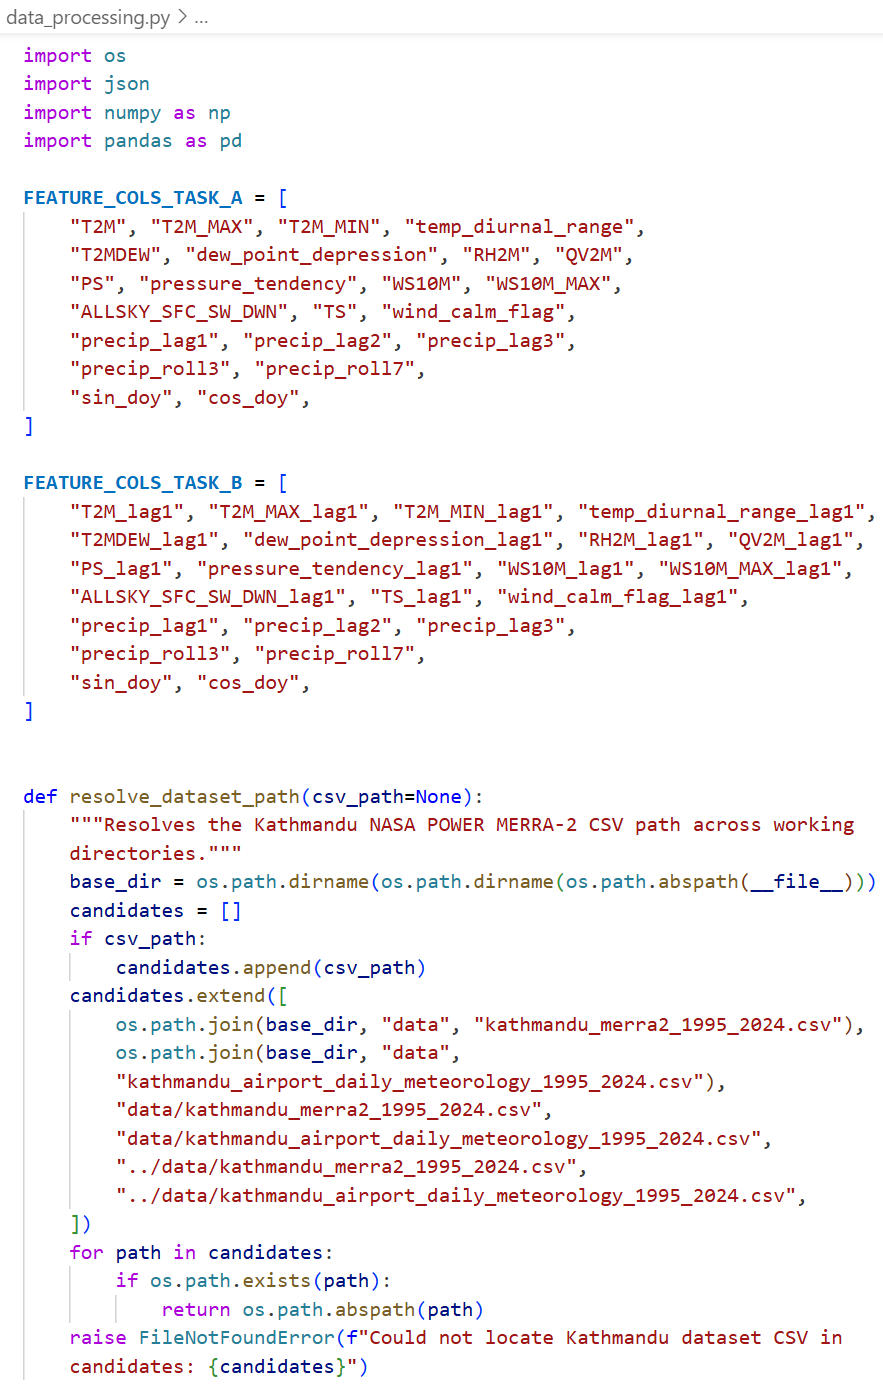
\includegraphics[width=\textwidth,height=0.33\textheight,keepaspectratio]{../figures/data_processing1.png}
\end{minipage}\hfill
\begin{minipage}[t]{0.475\textwidth}\vspace{0pt}
    \centering
    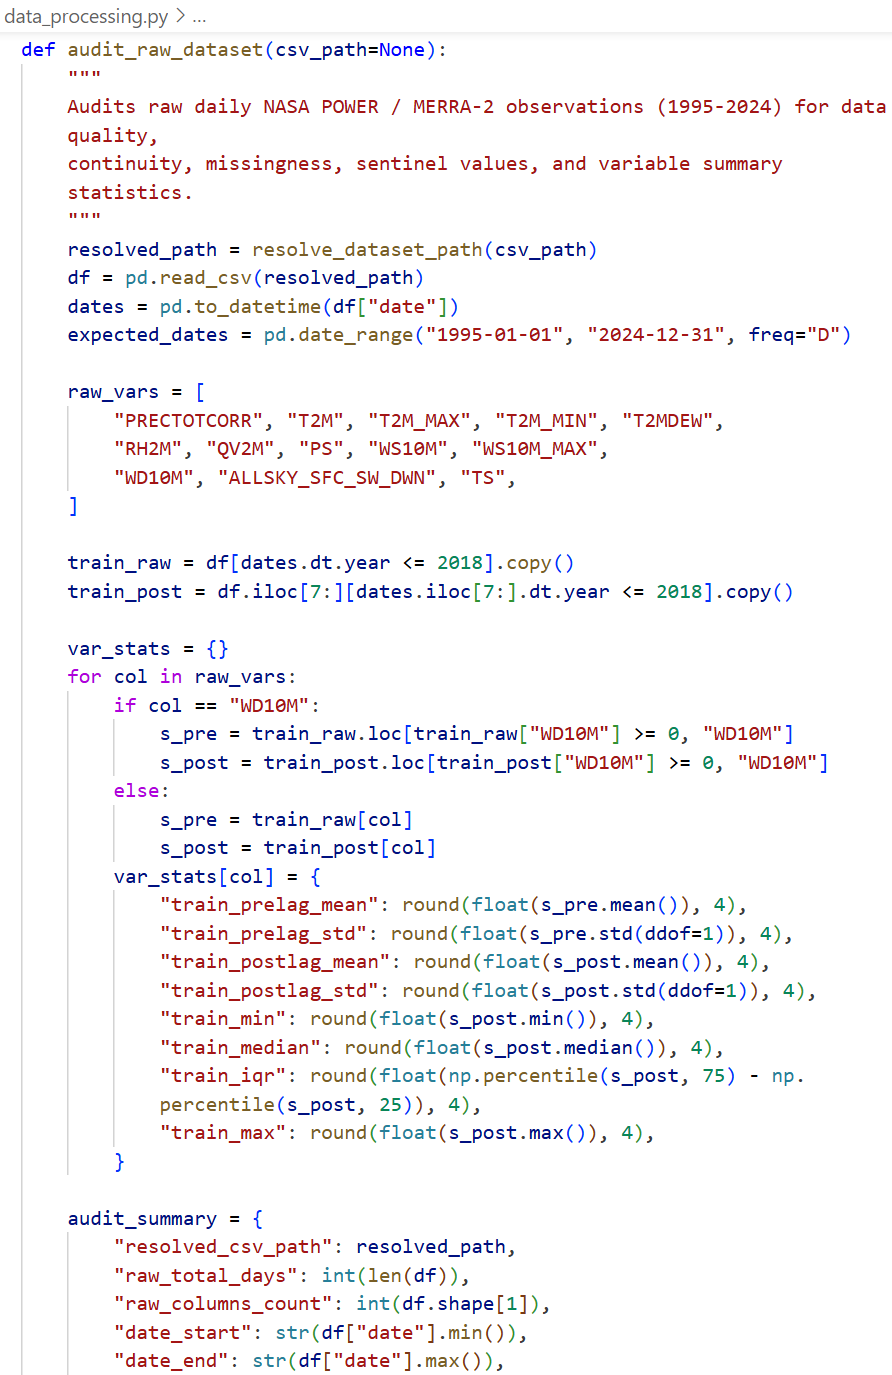
\includegraphics[width=\textwidth,height=0.33\textheight,keepaspectratio]{../figures/data_processing2.png}
\end{minipage}
\vspace{2.8em}
\noindent
\begin{minipage}[t]{0.475\textwidth}\vspace{0pt}
    \centering
    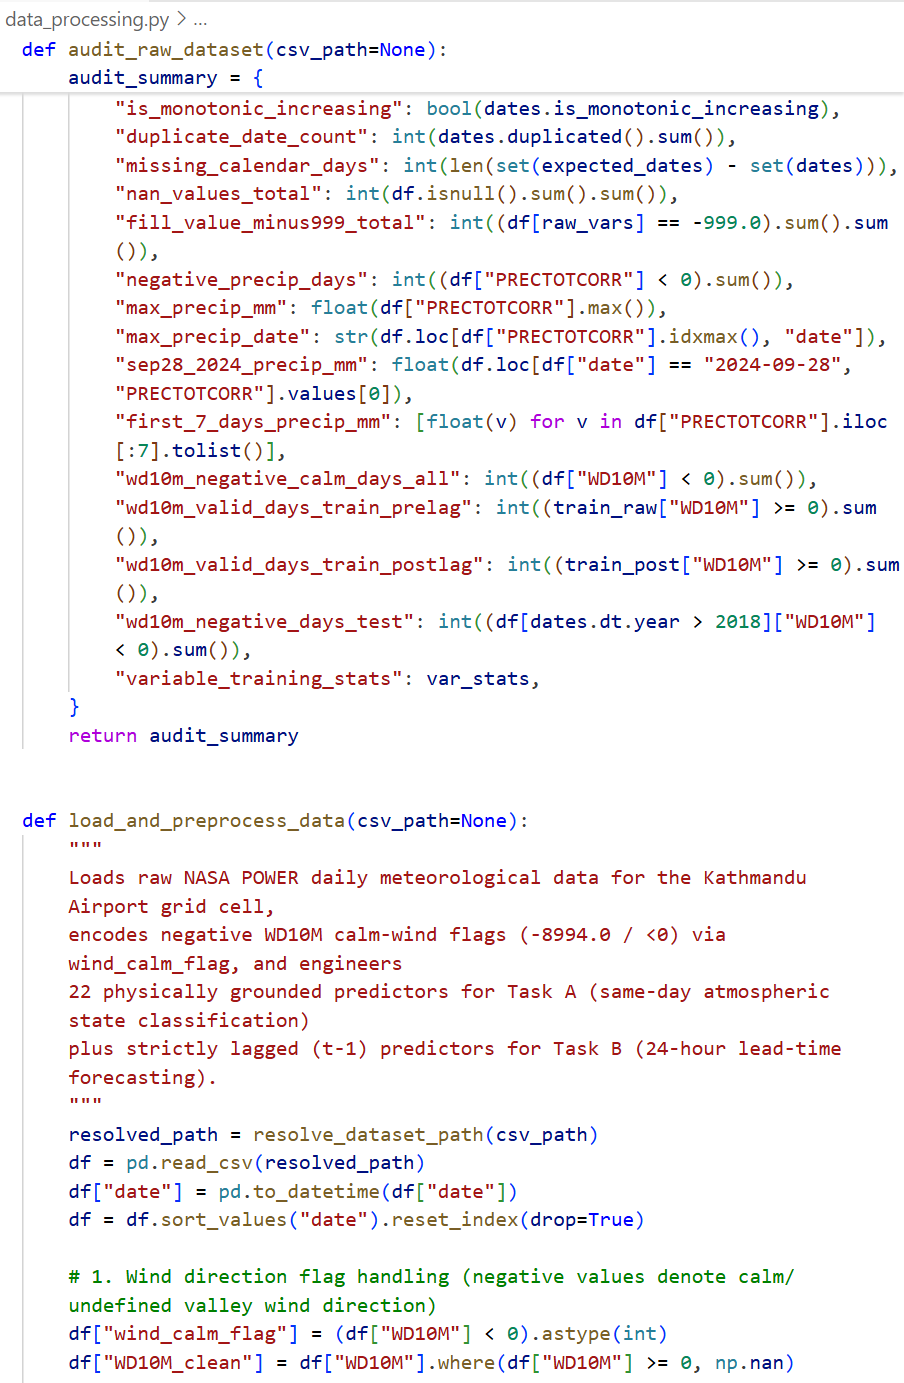
\includegraphics[width=\textwidth,height=0.33\textheight,keepaspectratio]{../figures/data_processing3.png}
\end{minipage}\hfill
\begin{minipage}[t]{0.475\textwidth}\vspace{0pt}
    \centering
    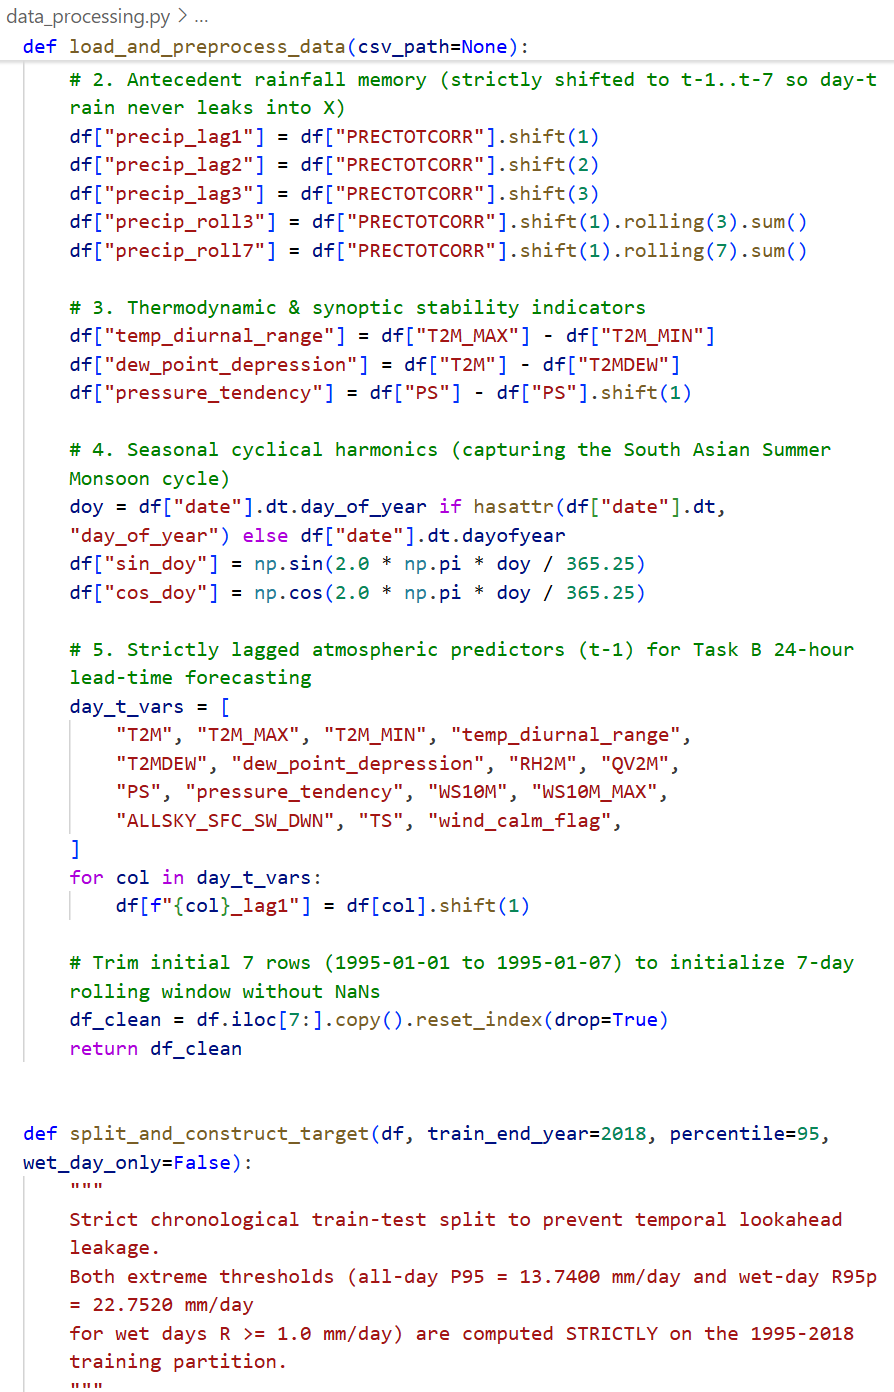
\includegraphics[width=\textwidth,height=0.33\textheight,keepaspectratio]{../figures/data_processing4.png}
\end{minipage}
\clearpage
\noindent
\begin{minipage}[t]{0.475\textwidth}\vspace{0pt}
    \centering
    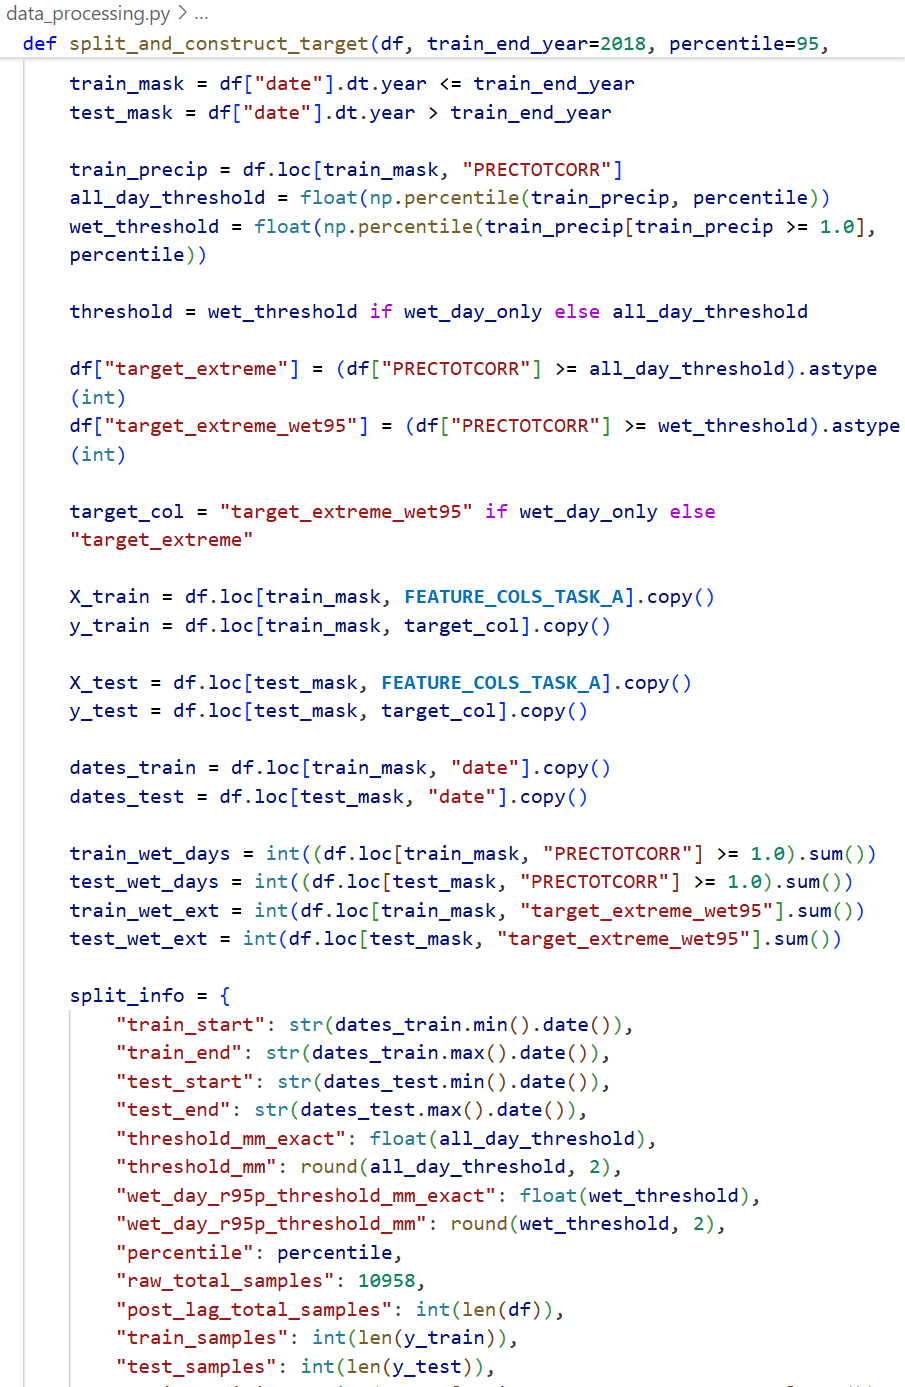
\includegraphics[width=\textwidth,height=0.33\textheight,keepaspectratio]{../figures/data_processing5.png}
\end{minipage}\hfill
\begin{minipage}[t]{0.475\textwidth}\vspace{0pt}
    \centering
    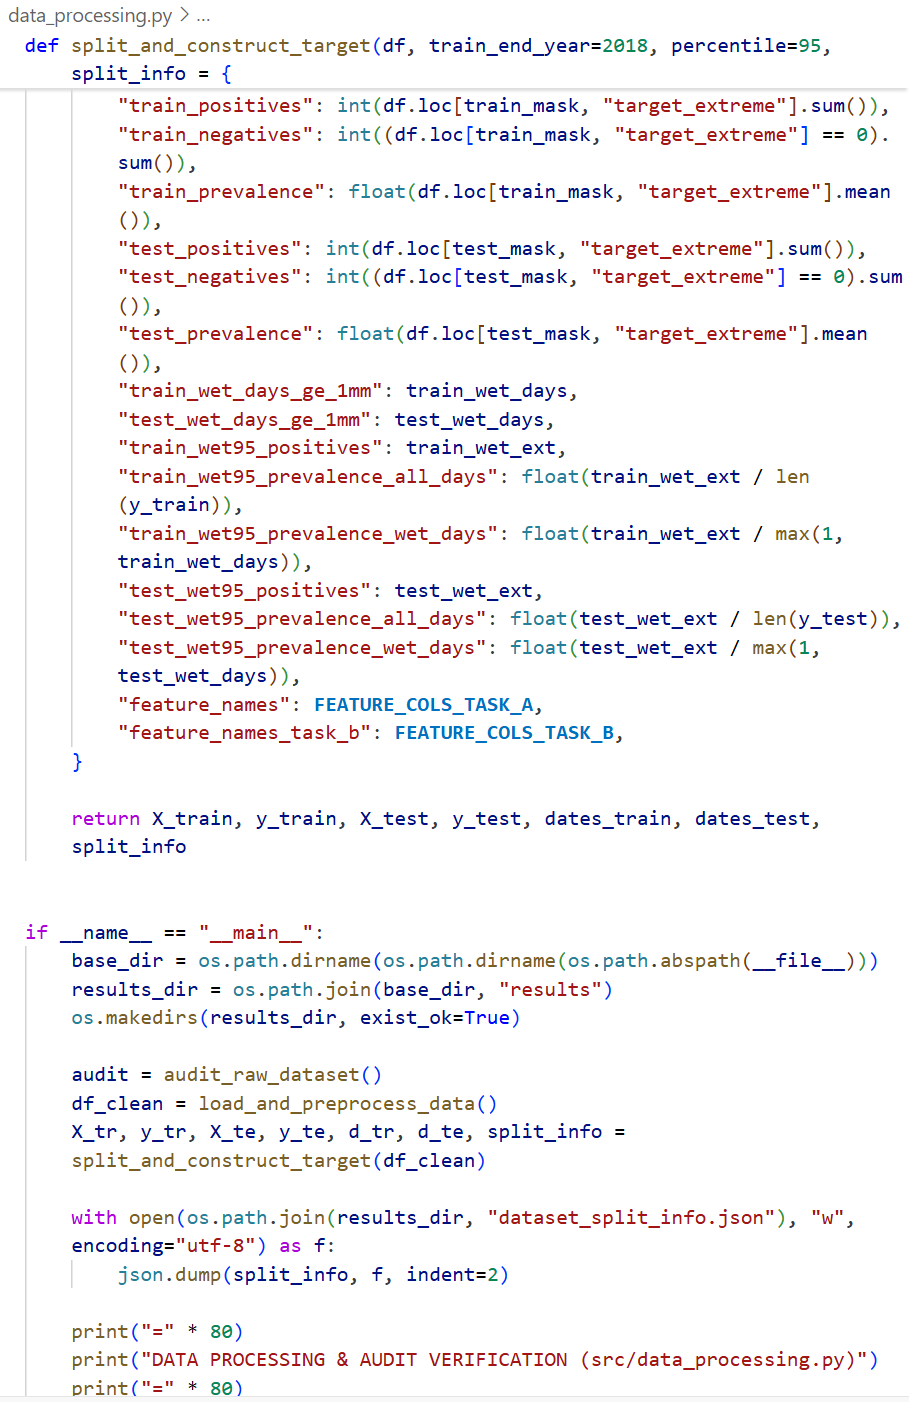
\includegraphics[width=\textwidth,height=0.33\textheight,keepaspectratio]{../figures/data_processing6.png}
\end{minipage}
\vspace{2.8em}
\noindent
\begin{minipage}[t]{0.475\textwidth}\vspace{0pt}
    \centering
    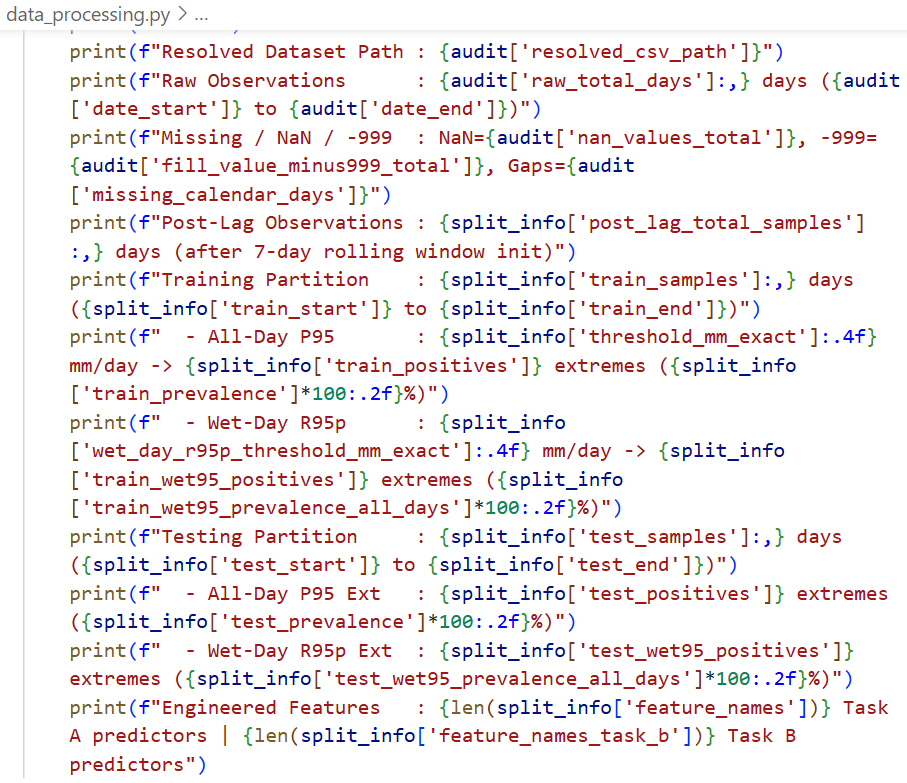
\includegraphics[width=\textwidth,height=0.33\textheight,keepaspectratio]{../figures/data_processing7.png}
\end{minipage}\hfill
\begin{minipage}[t]{0.475\textwidth}\vspace{0pt}
    \mbox{}
\end{minipage}
\vspace{2.4em}

\subsection*{B.\quad MODEL TRAINING AND EVALUATION IMPLEMENTATION}
\vspace{0.6em}

\noindent
\begin{minipage}[t]{0.475\textwidth}\vspace{0pt}
    \centering
    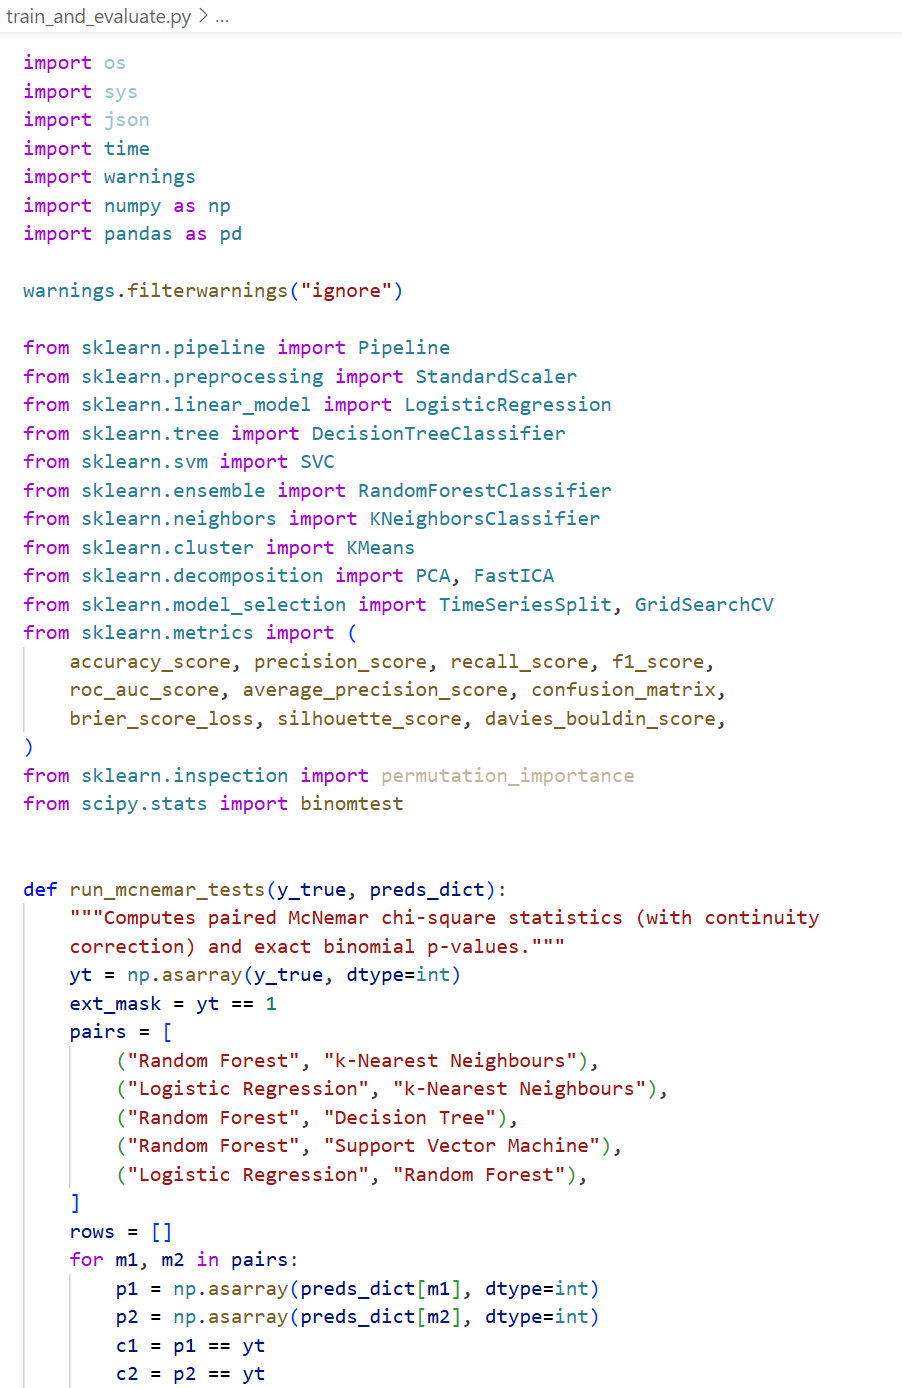
\includegraphics[width=\textwidth,height=0.33\textheight,keepaspectratio]{../figures/train_and_evaluate1.png}
\end{minipage}\hfill
\begin{minipage}[t]{0.475\textwidth}\vspace{0pt}
    \centering
    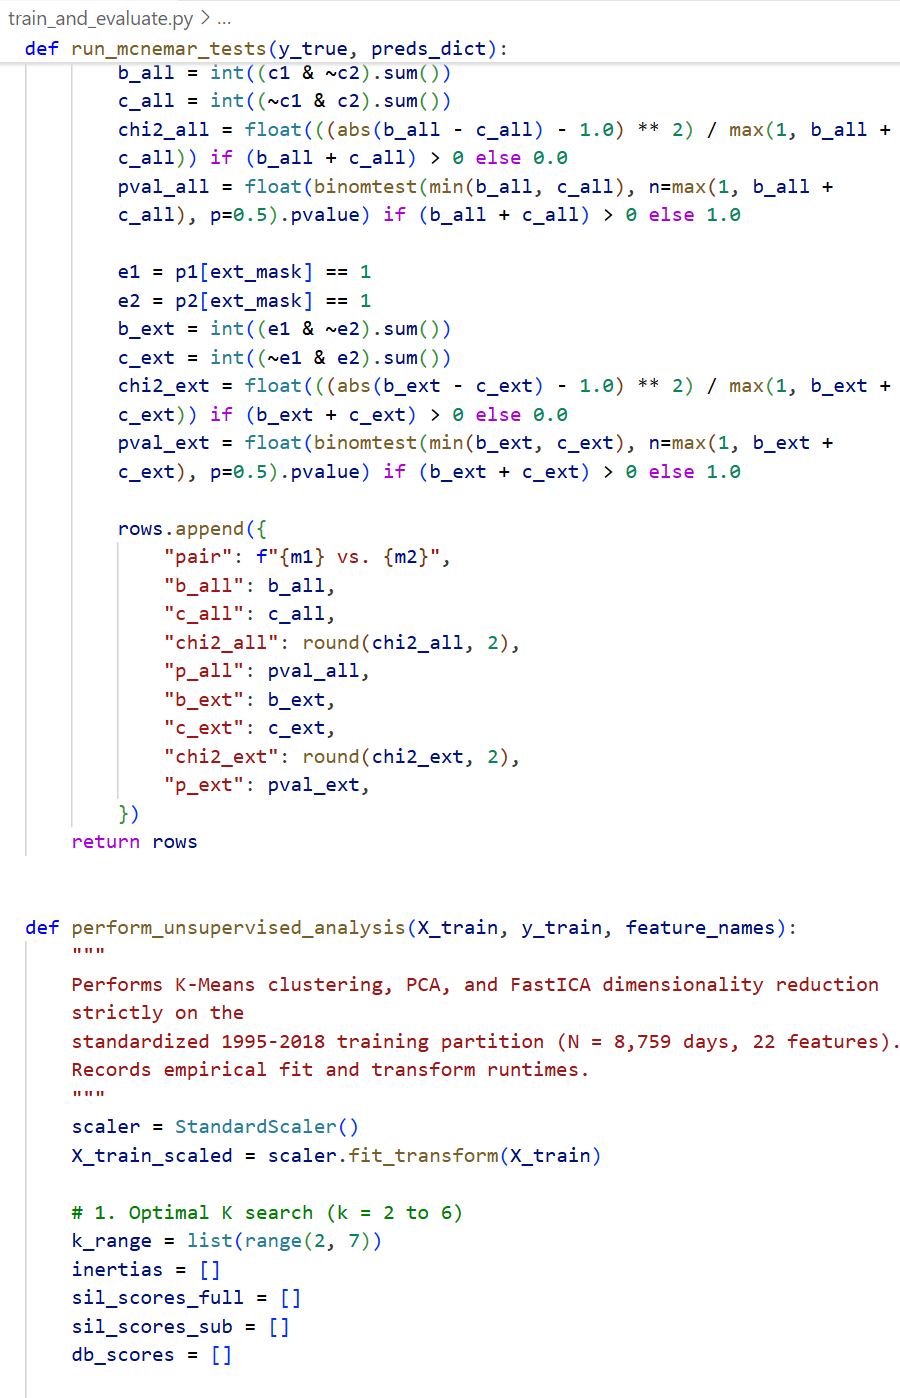
\includegraphics[width=\textwidth,height=0.33\textheight,keepaspectratio]{../figures/train_and_evaluate2.png}
\end{minipage}
\clearpage
\noindent
\begin{minipage}[t]{0.475\textwidth}\vspace{0pt}
    \centering
    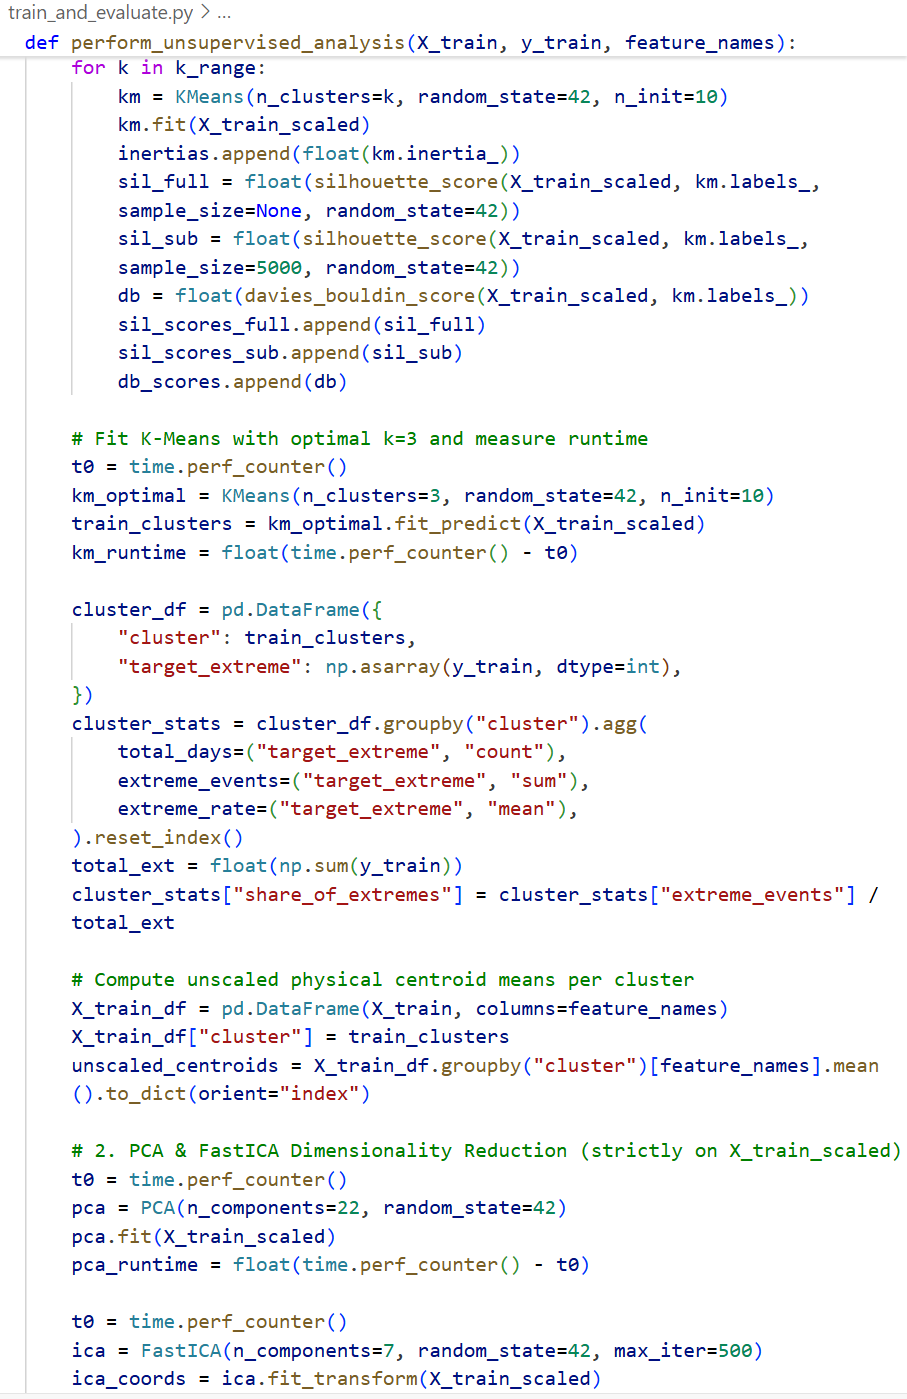
\includegraphics[width=\textwidth,height=0.33\textheight,keepaspectratio]{../figures/train_and_evaluate3.png}
\end{minipage}\hfill
\begin{minipage}[t]{0.475\textwidth}\vspace{0pt}
    \centering
    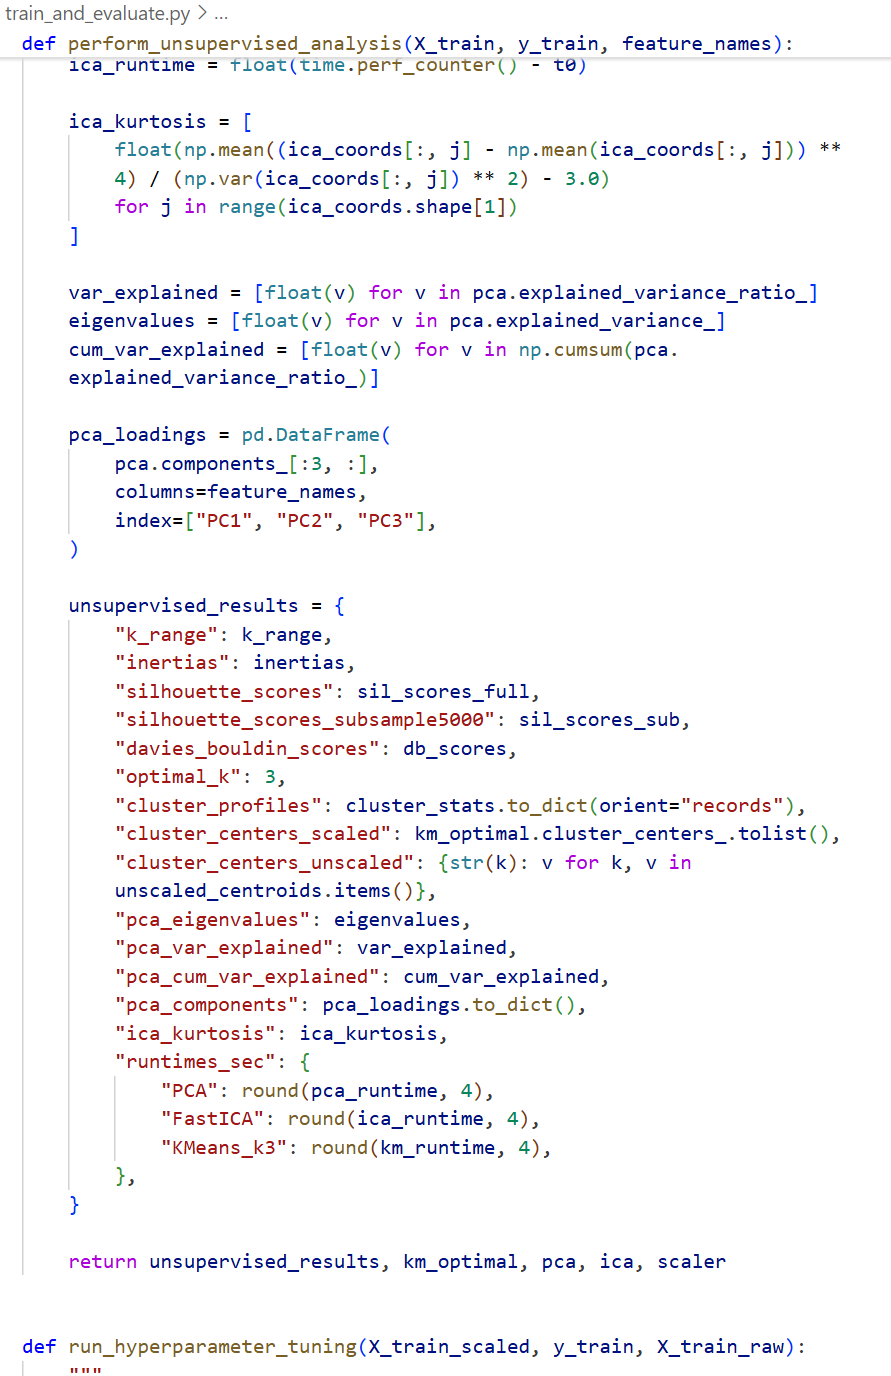
\includegraphics[width=\textwidth,height=0.33\textheight,keepaspectratio]{../figures/train_and_evaluate4.png}
\end{minipage}
\vspace{2.8em}
\noindent
\begin{minipage}[t]{0.475\textwidth}\vspace{0pt}
    \centering
    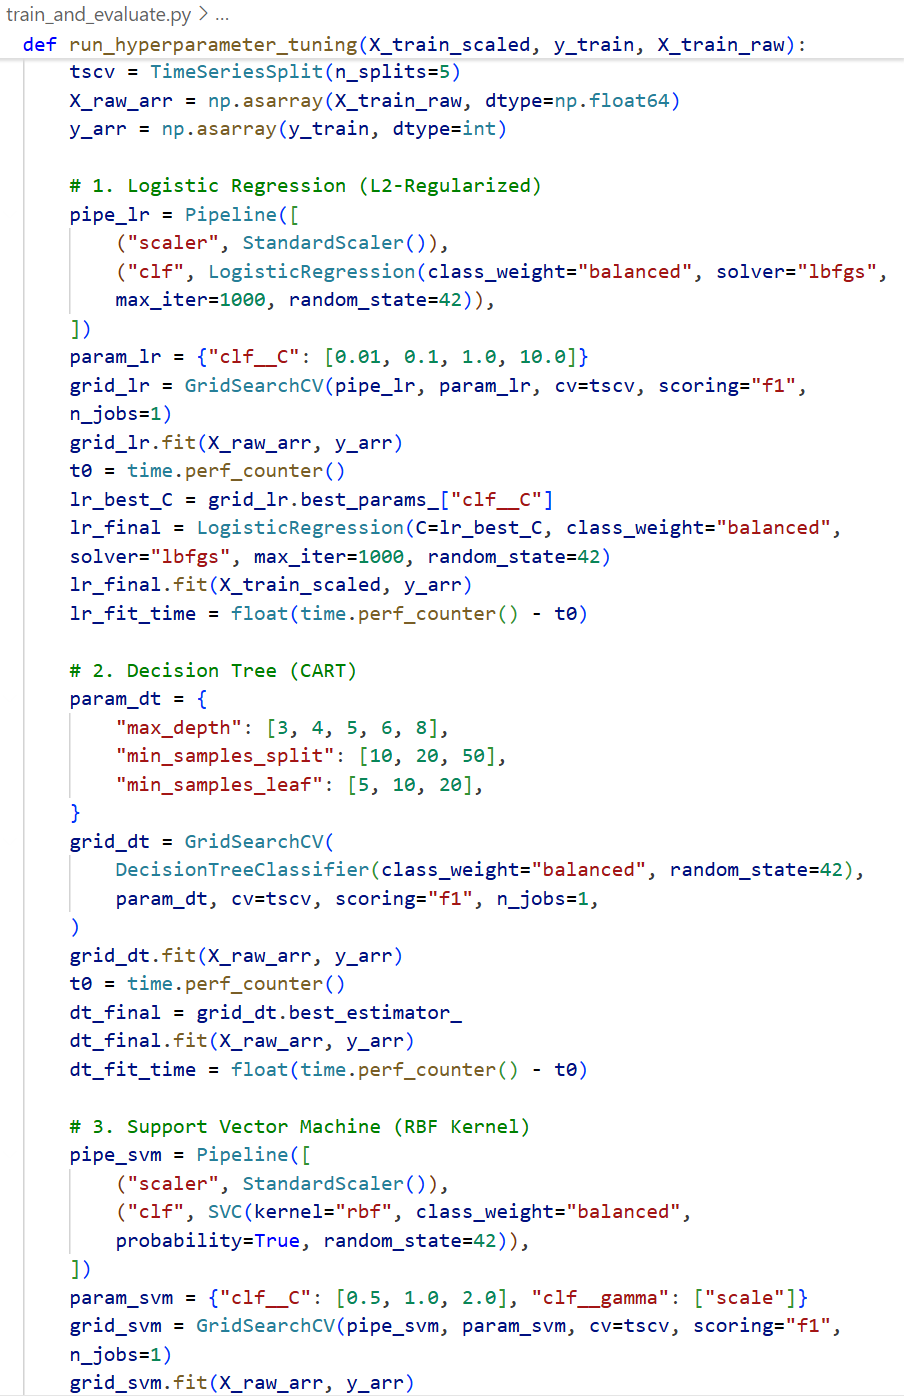
\includegraphics[width=\textwidth,height=0.33\textheight,keepaspectratio]{../figures/train_and_evaluate5.png}
\end{minipage}\hfill
\begin{minipage}[t]{0.475\textwidth}\vspace{0pt}
    \centering
    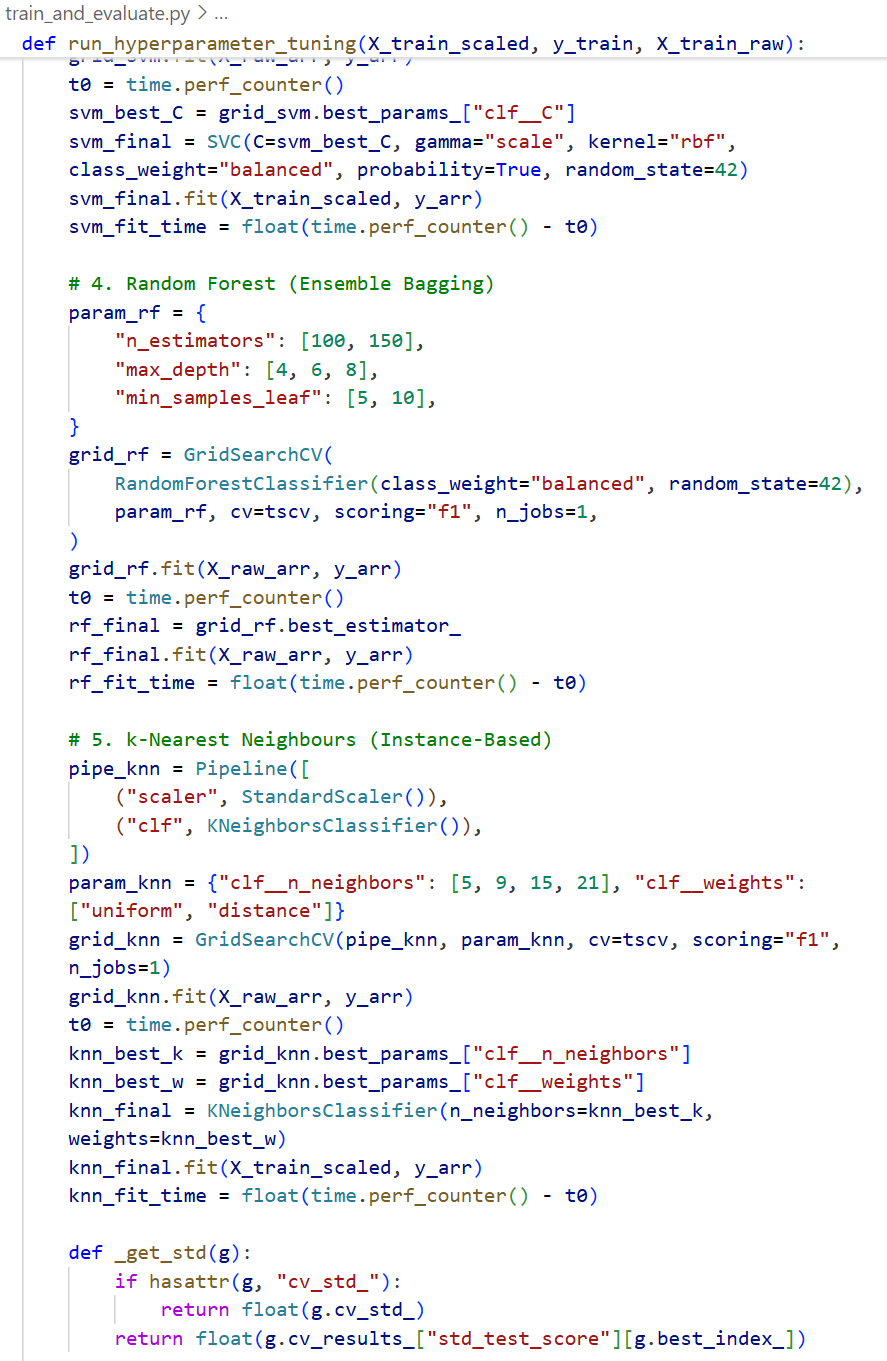
\includegraphics[width=\textwidth,height=0.33\textheight,keepaspectratio]{../figures/train_and_evaluate6.png}
\end{minipage}
\clearpage
\noindent
\begin{minipage}[t]{0.475\textwidth}\vspace{0pt}
    \centering
    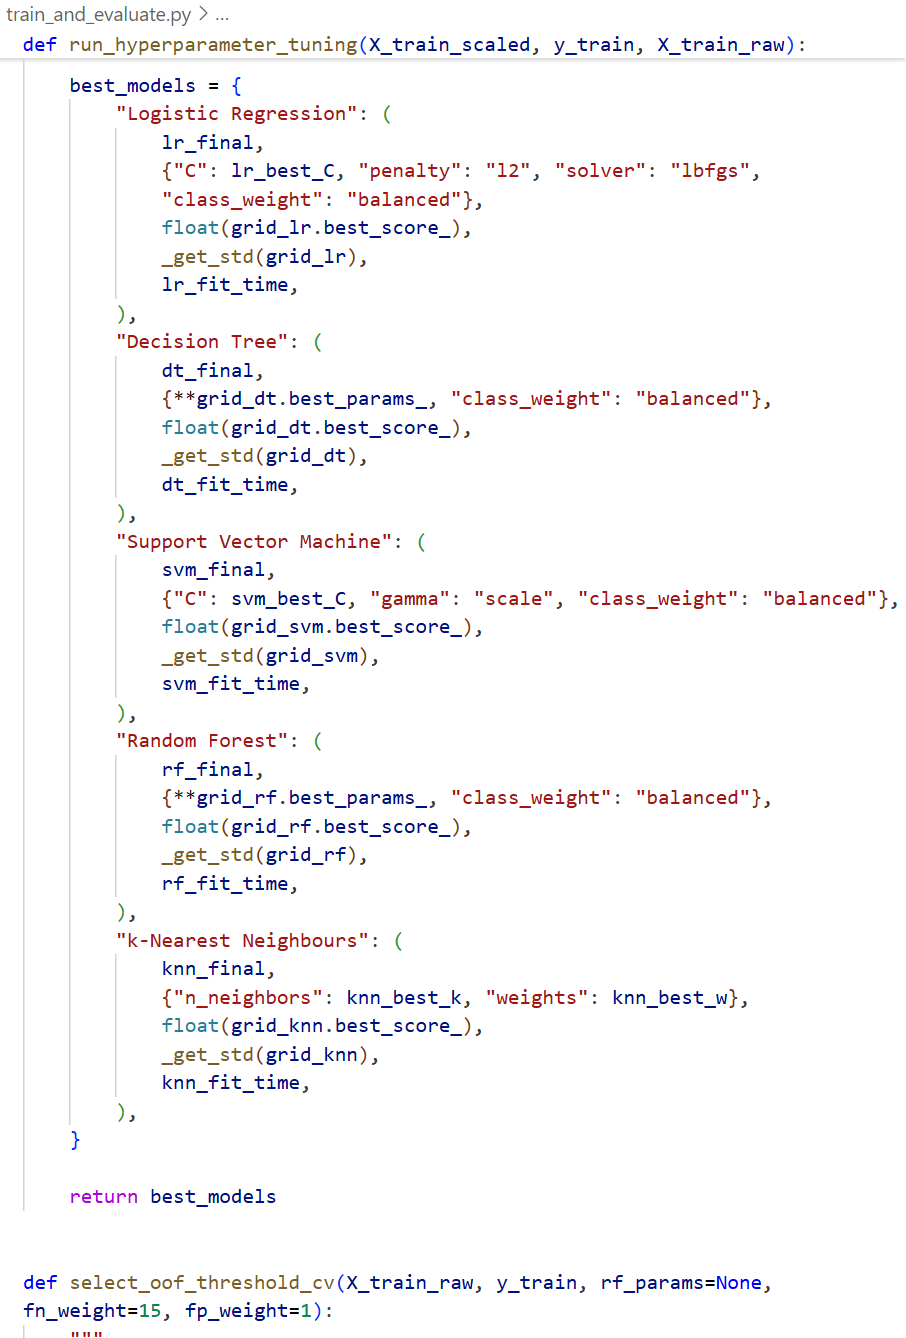
\includegraphics[width=\textwidth,height=0.33\textheight,keepaspectratio]{../figures/train_and_evaluate7.png}
\end{minipage}\hfill
\begin{minipage}[t]{0.475\textwidth}\vspace{0pt}
    \centering
    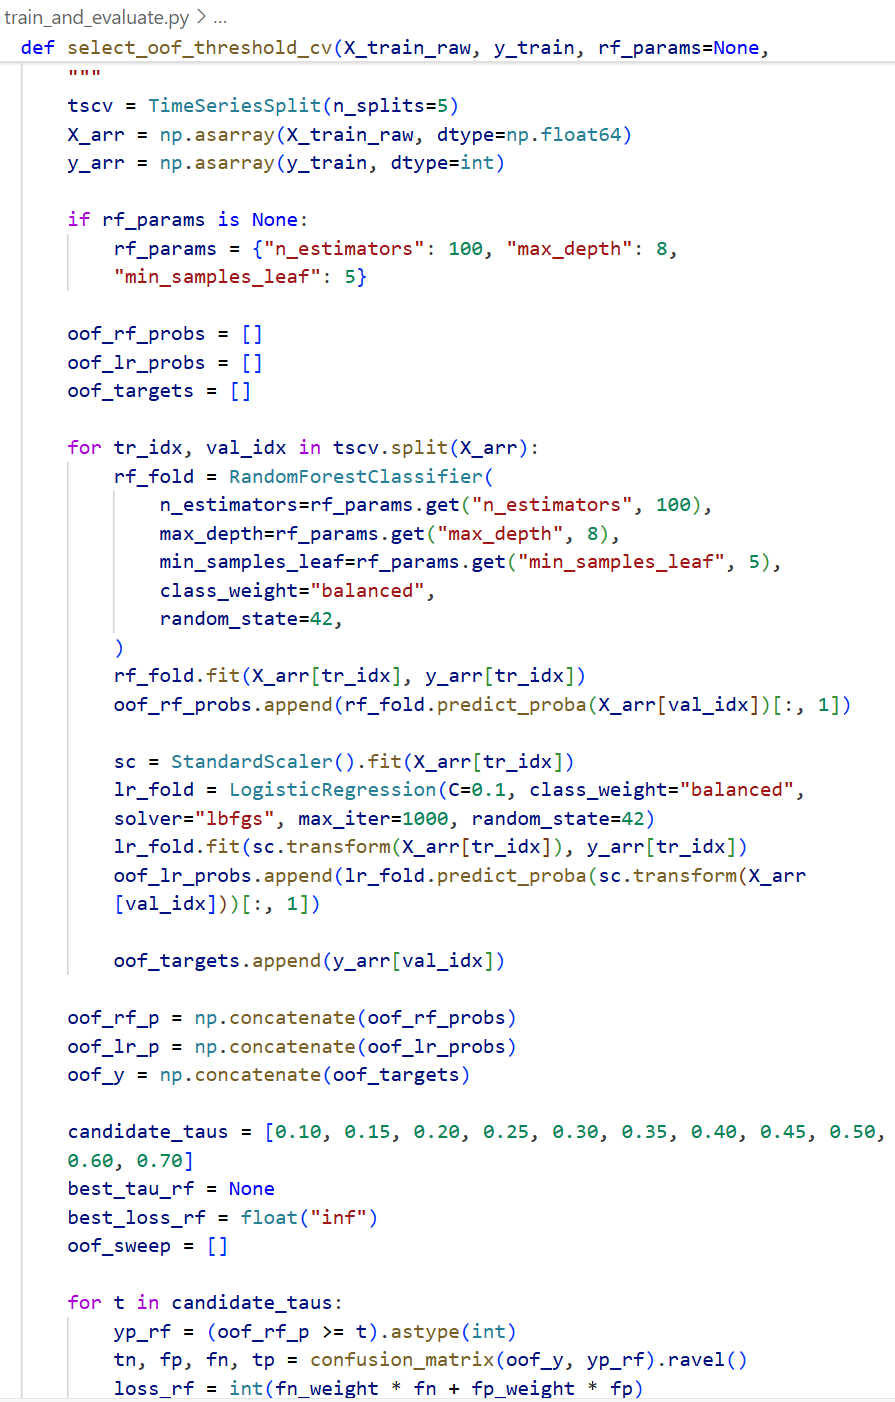
\includegraphics[width=\textwidth,height=0.33\textheight,keepaspectratio]{../figures/train_and_evaluate8.png}
\end{minipage}
\vspace{2.8em}
\noindent
\begin{minipage}[t]{0.475\textwidth}\vspace{0pt}
    \centering
    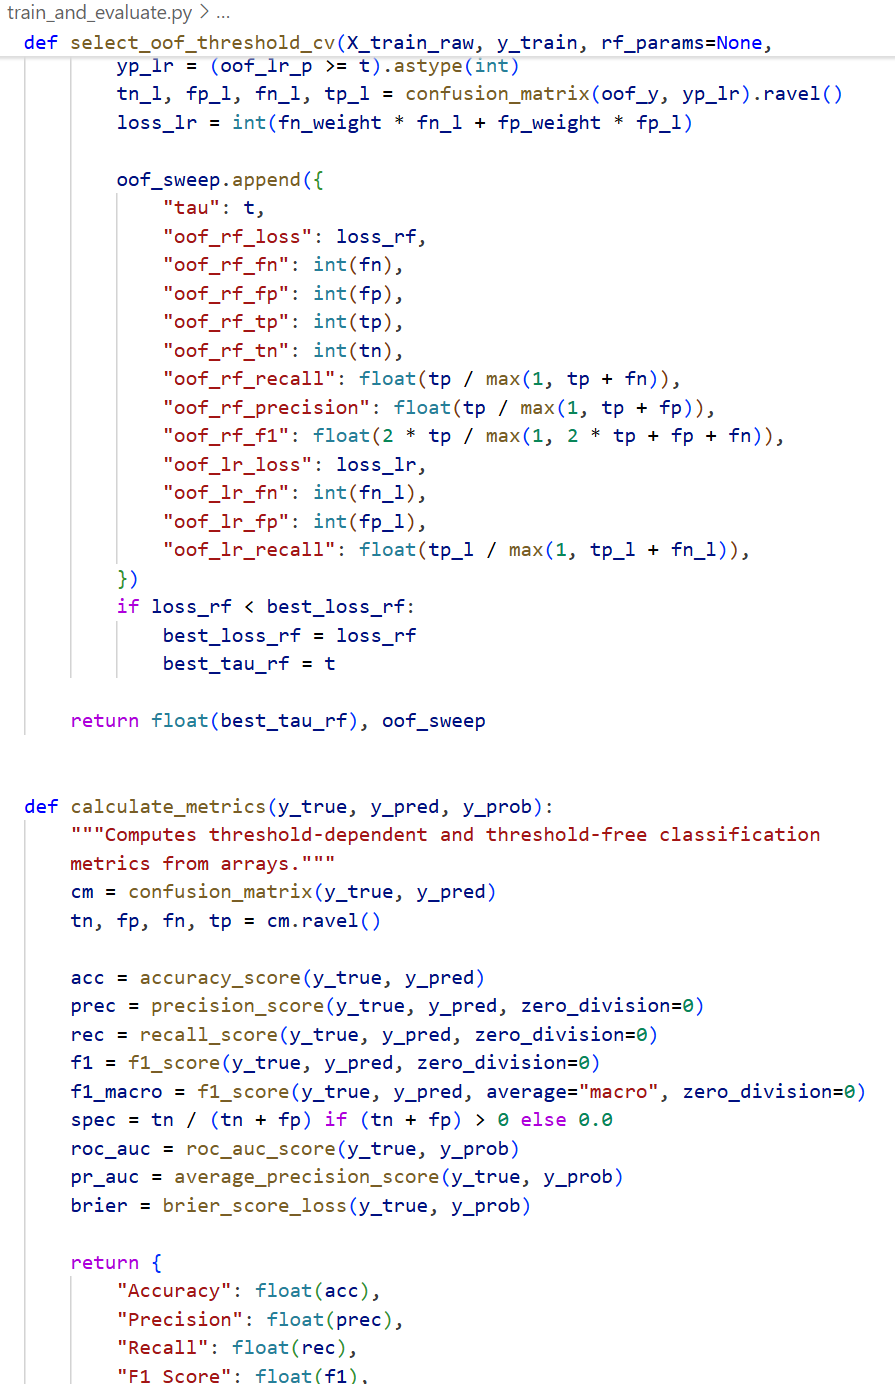
\includegraphics[width=\textwidth,height=0.33\textheight,keepaspectratio]{../figures/train_and_evaluate9.png}
\end{minipage}\hfill
\begin{minipage}[t]{0.475\textwidth}\vspace{0pt}
    \centering
    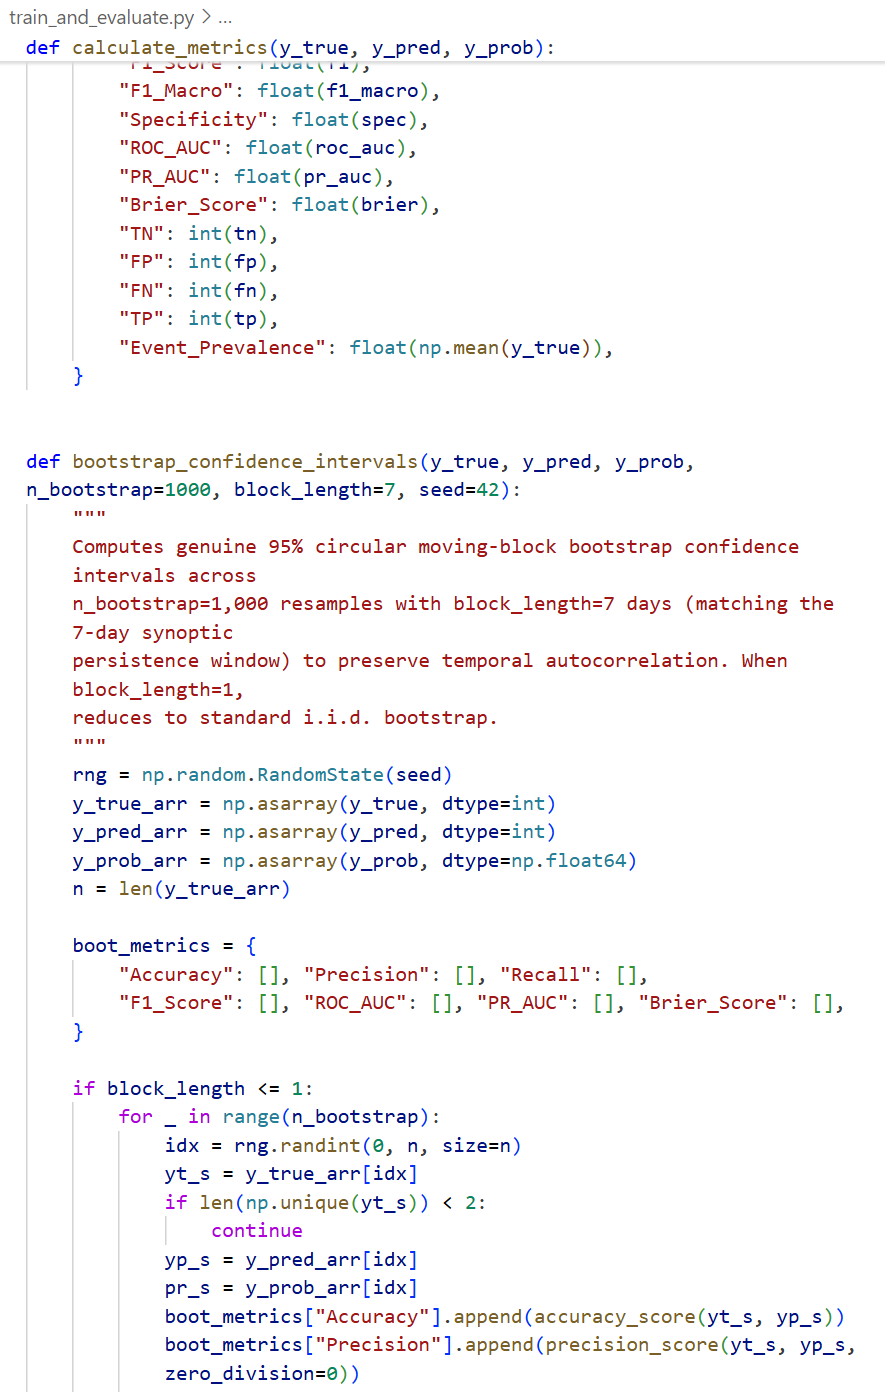
\includegraphics[width=\textwidth,height=0.33\textheight,keepaspectratio]{../figures/train_and_evaluate10.png}
\end{minipage}
\clearpage
\noindent
\begin{minipage}[t]{0.475\textwidth}\vspace{0pt}
    \centering
    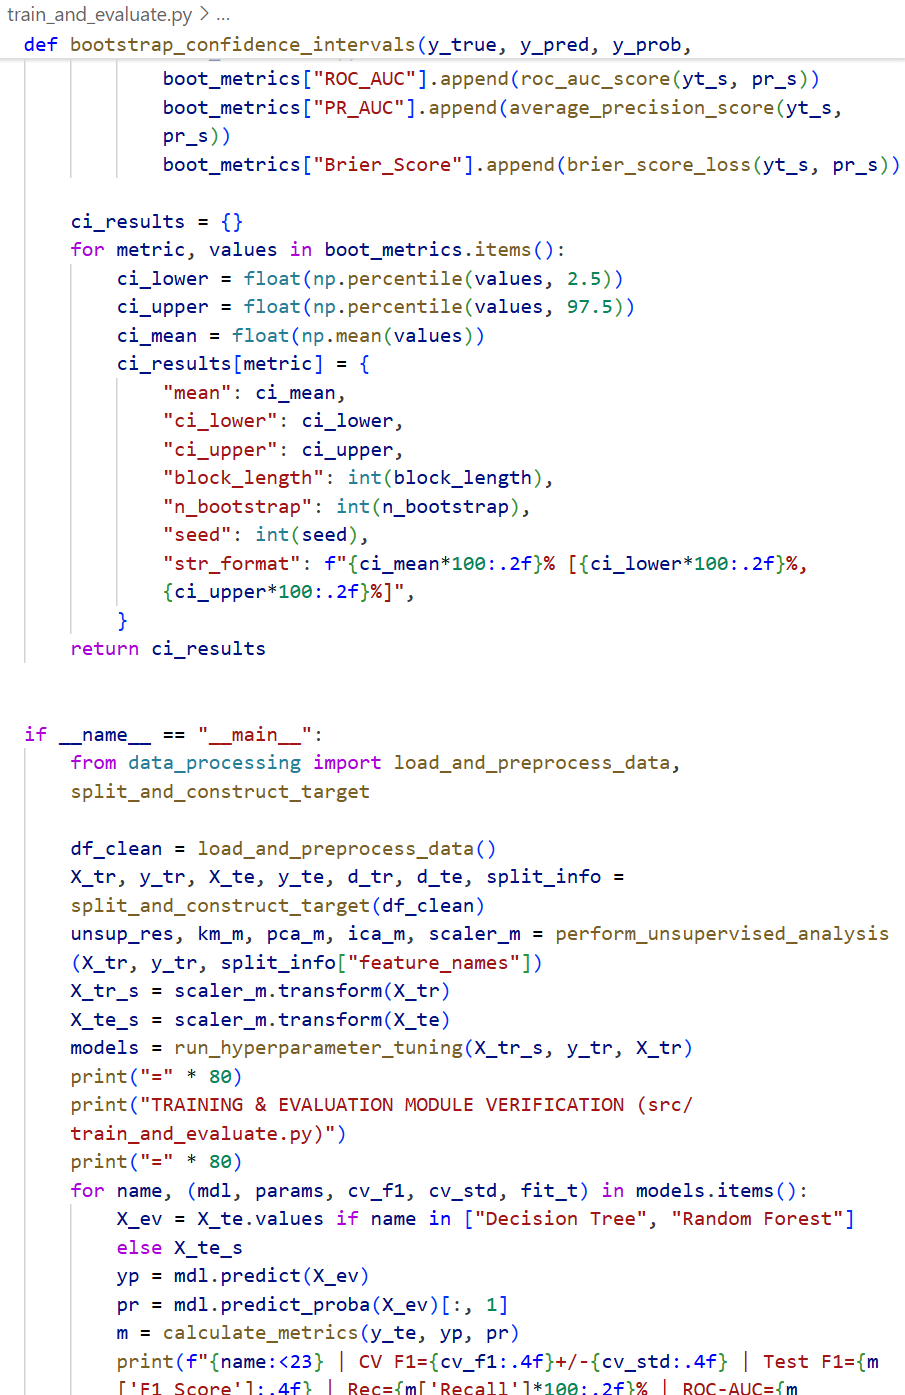
\includegraphics[width=\textwidth,height=0.33\textheight,keepaspectratio]{../figures/train_and_evaluate11.png}
\end{minipage}\hfill
\begin{minipage}[t]{0.475\textwidth}\vspace{0pt}
    \mbox{}
\end{minipage}
\vspace{2.4em}

\subsection*{C.\quad VISUAL ANALYTICS AND DIAGNOSTIC RESULTS}
\vspace{0.6em}

\noindent
\begin{minipage}[t]{0.475\textwidth}\vspace{0pt}
    \centering
    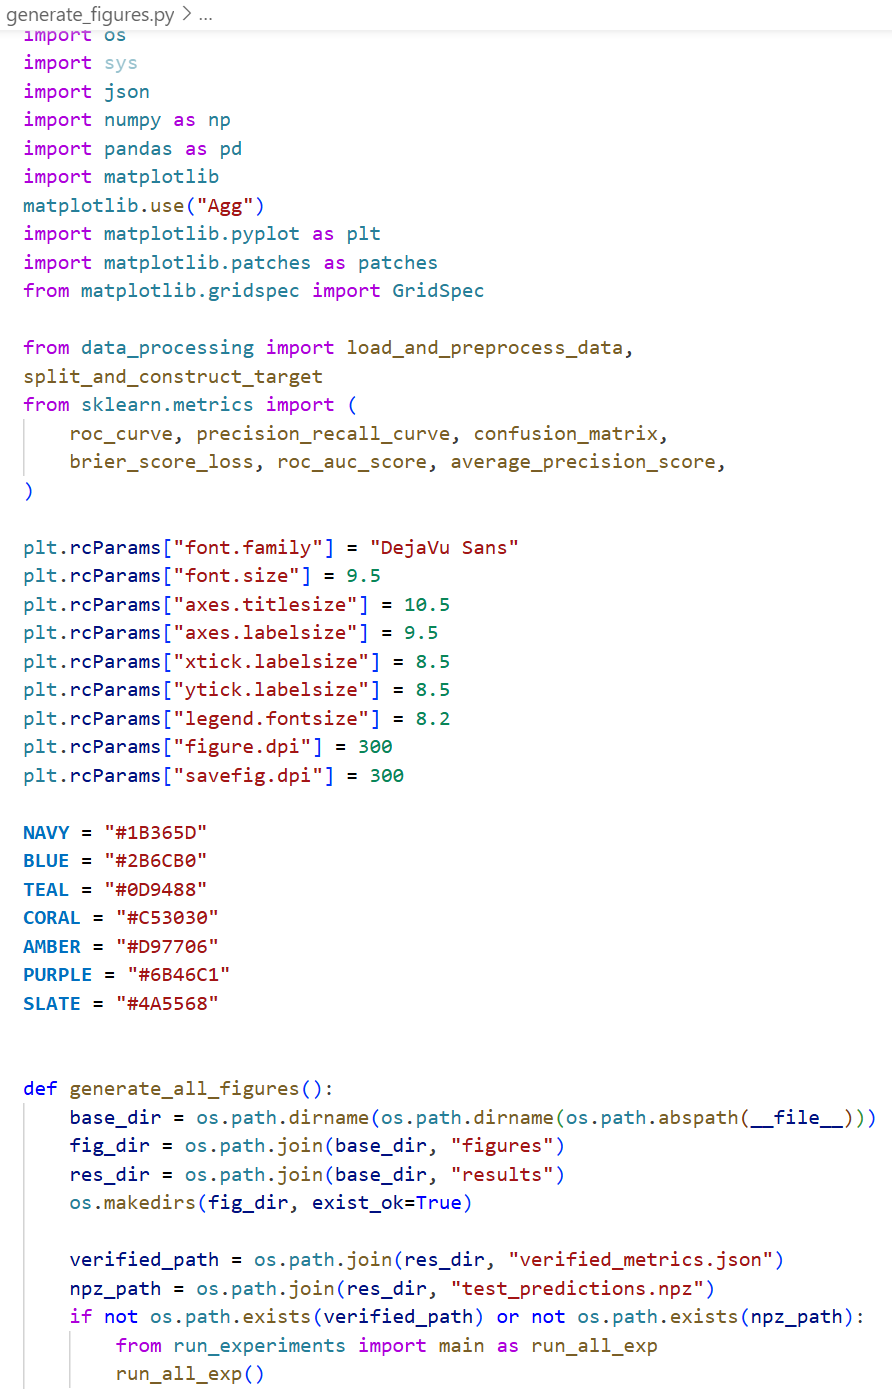
\includegraphics[width=\textwidth,height=0.33\textheight,keepaspectratio]{../figures/generate_figures1.png}
\end{minipage}\hfill
\begin{minipage}[t]{0.475\textwidth}\vspace{0pt}
    \centering
    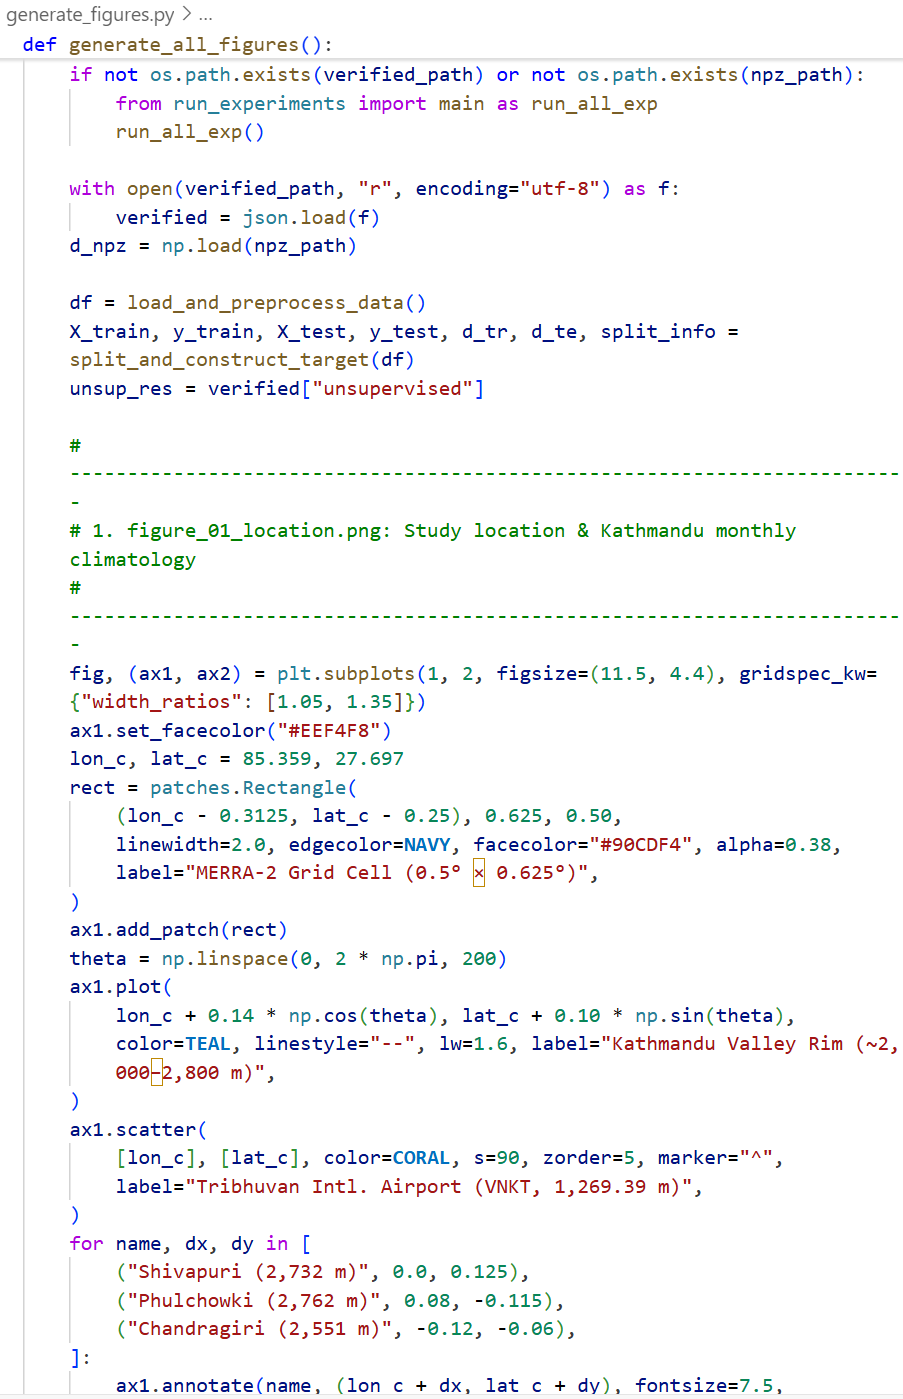
\includegraphics[width=\textwidth,height=0.33\textheight,keepaspectratio]{../figures/generate_figures2.png}
\end{minipage}
\clearpage
\noindent
\begin{minipage}[t]{0.475\textwidth}\vspace{0pt}
    \centering
    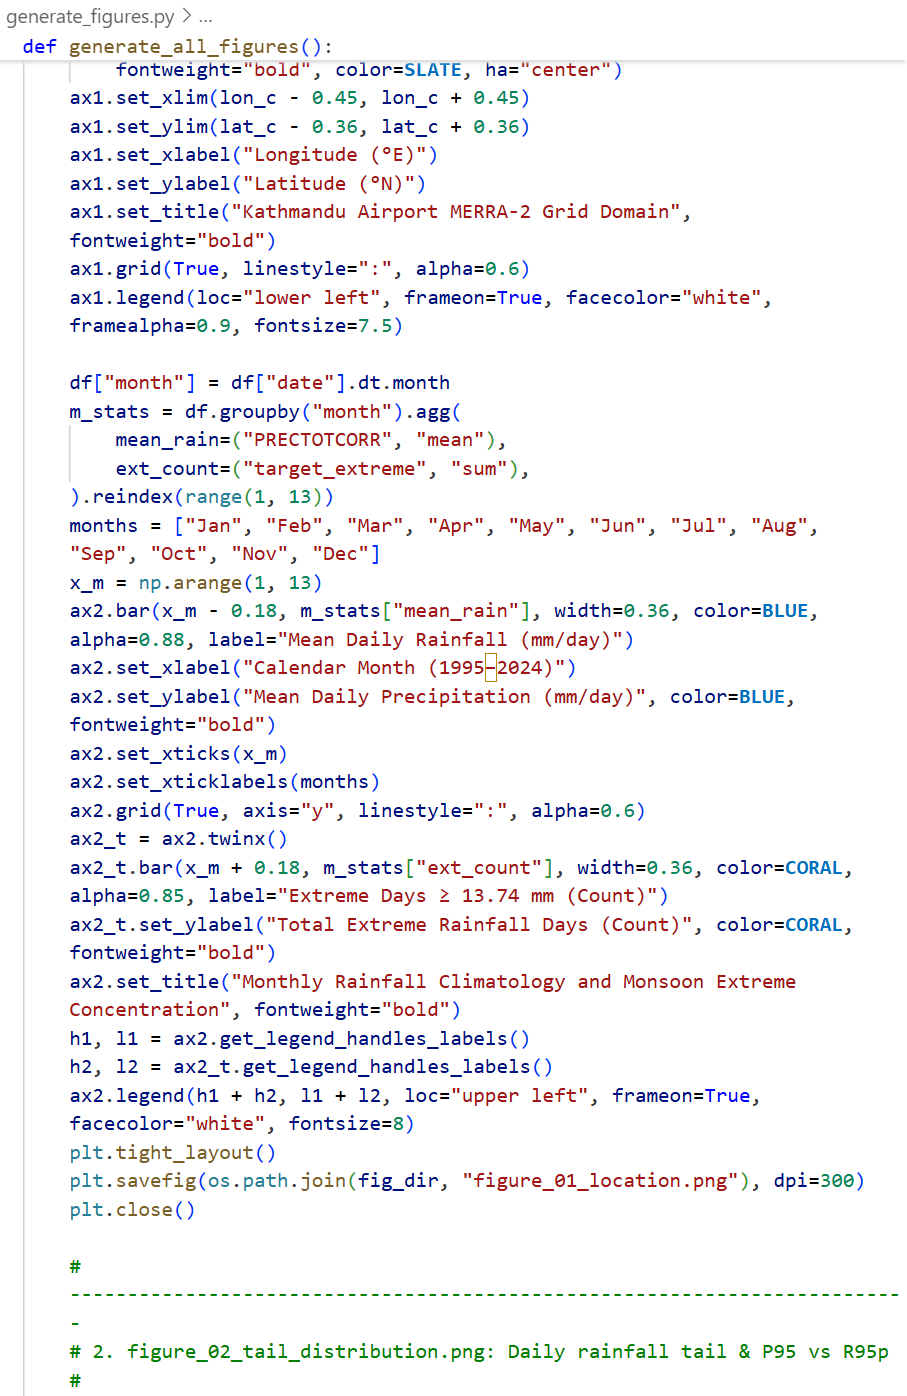
\includegraphics[width=\textwidth,height=0.33\textheight,keepaspectratio]{../figures/generate_figures3.png}
\end{minipage}\hfill
\begin{minipage}[t]{0.475\textwidth}\vspace{0pt}
    \centering
    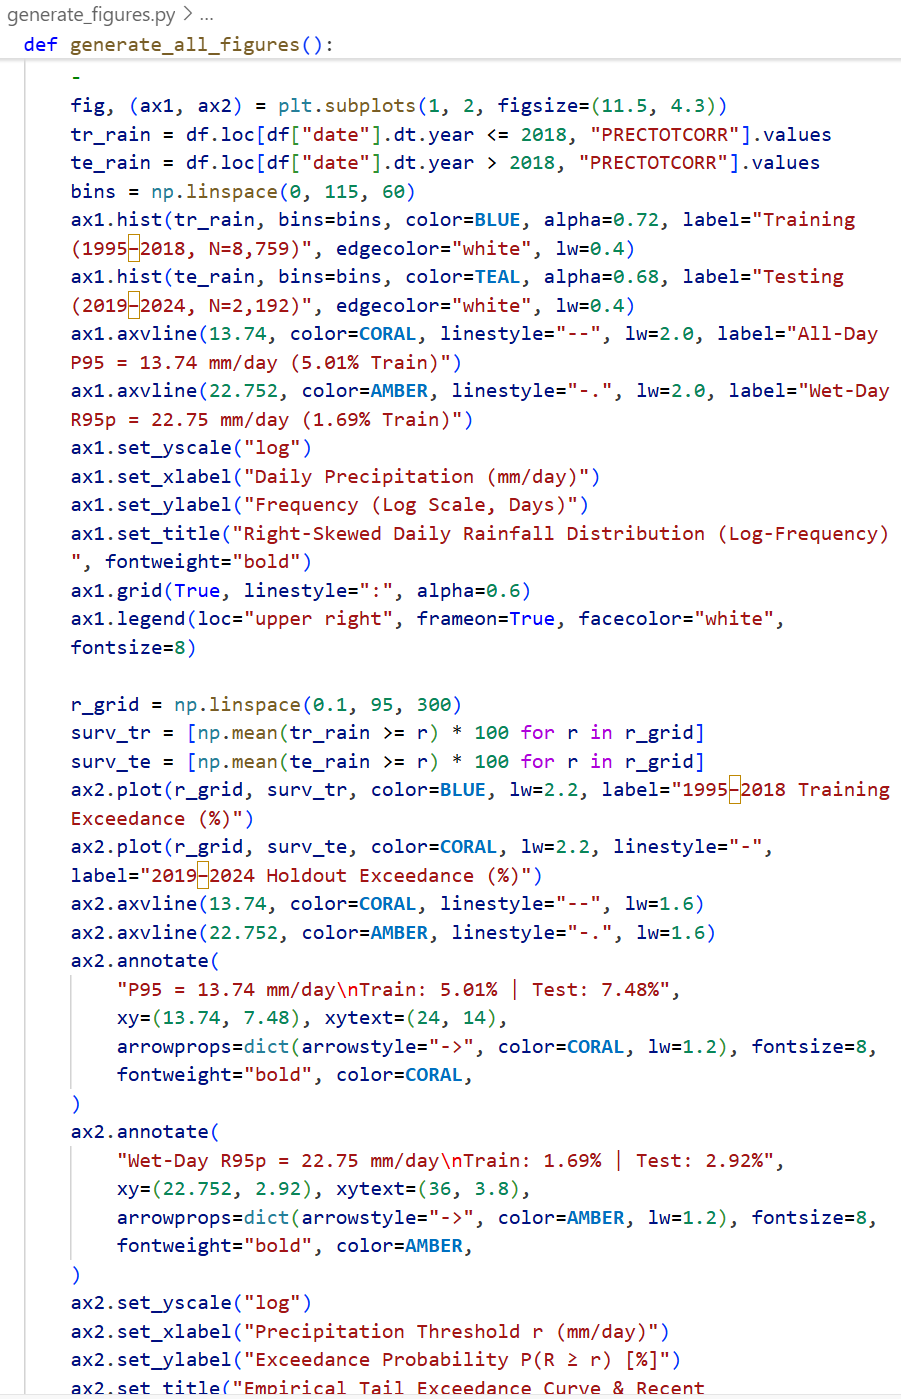
\includegraphics[width=\textwidth,height=0.33\textheight,keepaspectratio]{../figures/generate_figures4.png}
\end{minipage}
\vspace{2.8em}
\noindent
\begin{minipage}[t]{0.475\textwidth}\vspace{0pt}
    \centering
    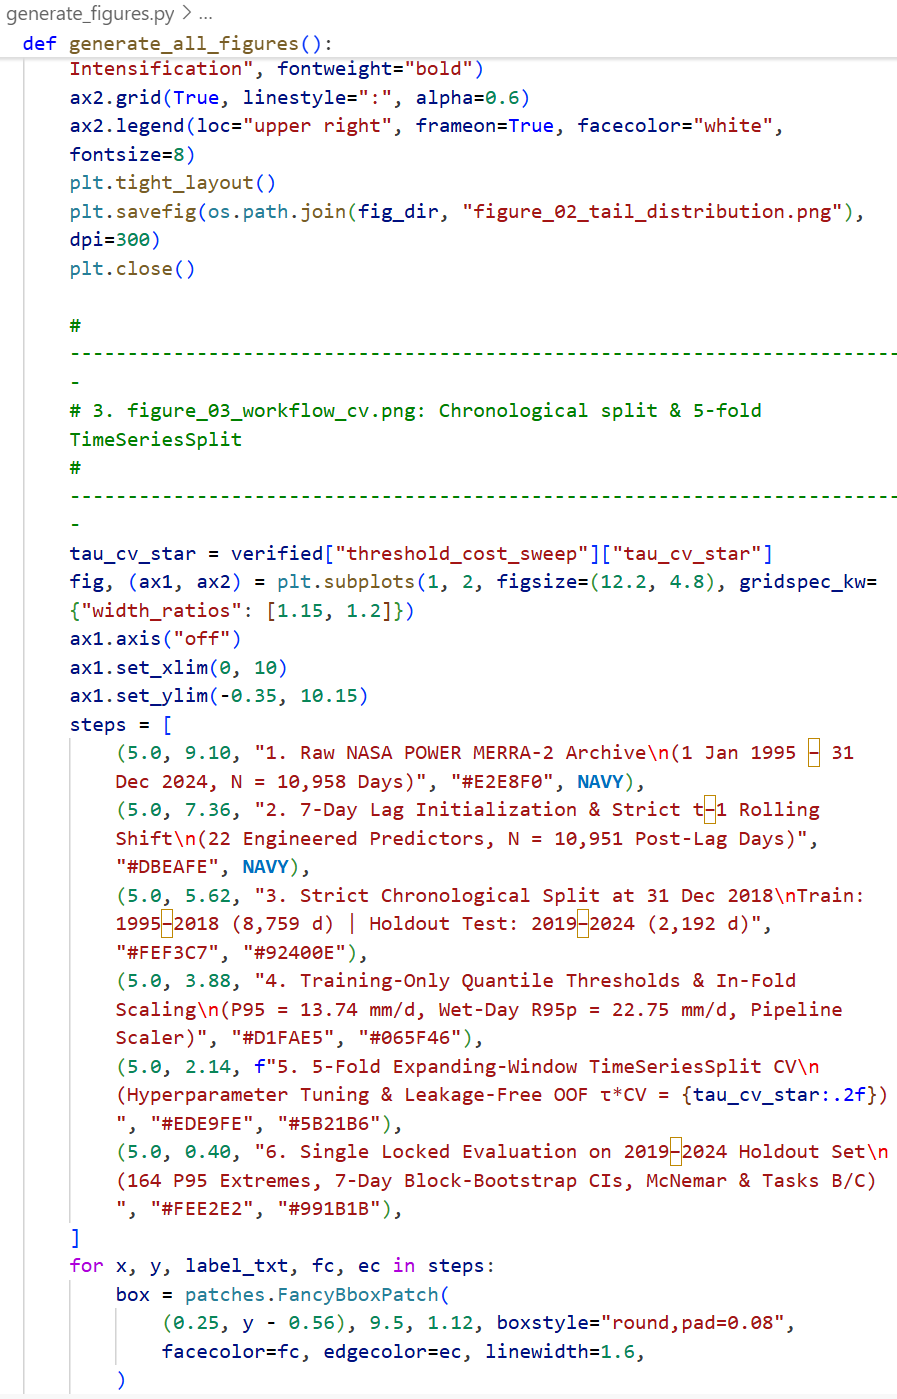
\includegraphics[width=\textwidth,height=0.33\textheight,keepaspectratio]{../figures/generate_figures5.png}
\end{minipage}\hfill
\begin{minipage}[t]{0.475\textwidth}\vspace{0pt}
    \centering
    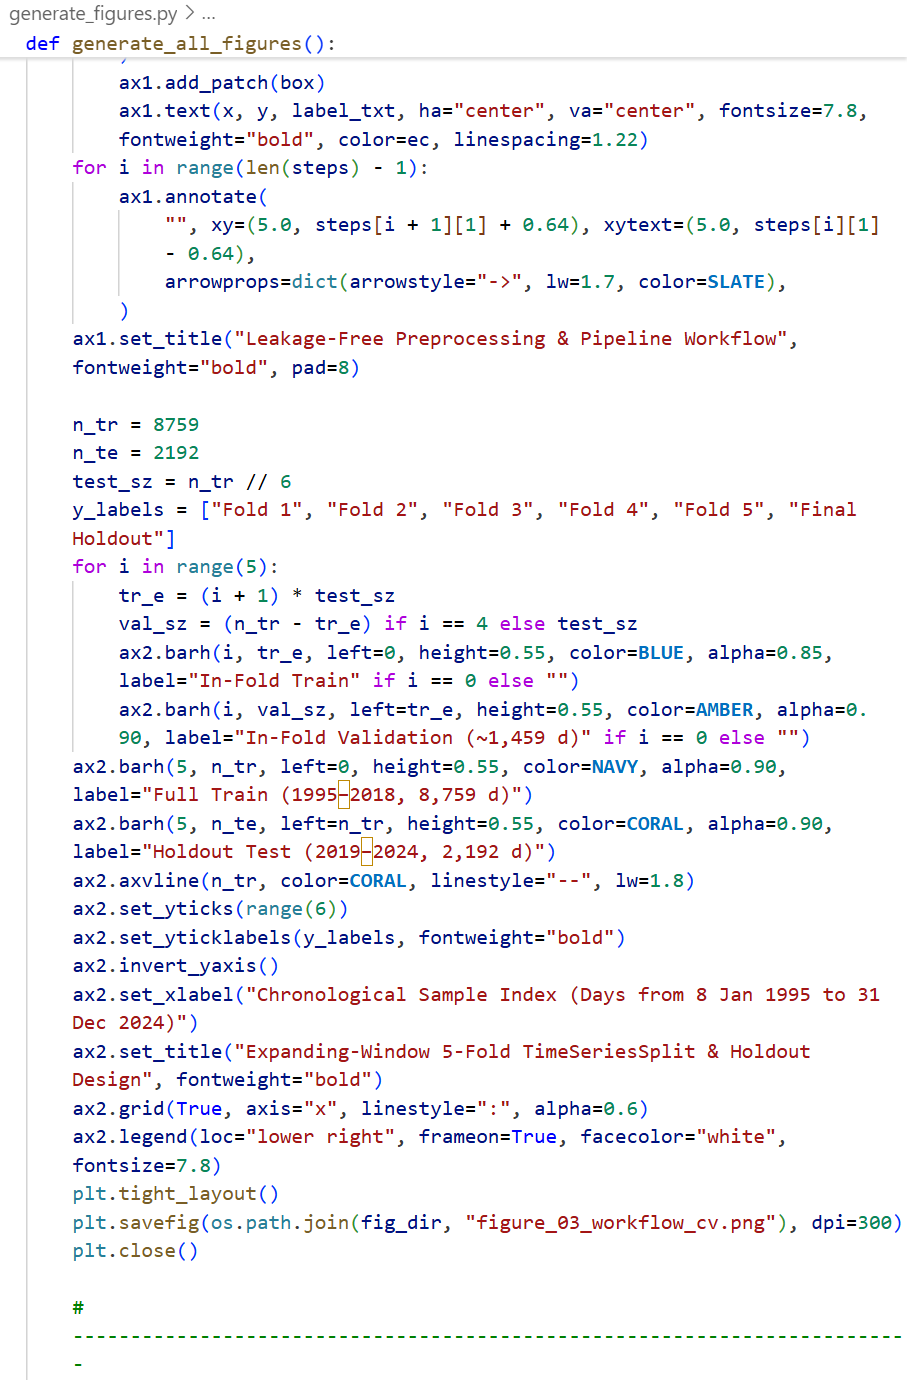
\includegraphics[width=\textwidth,height=0.33\textheight,keepaspectratio]{../figures/generate_figures6.png}
\end{minipage}
\clearpage
\noindent
\begin{minipage}[t]{0.475\textwidth}\vspace{0pt}
    \centering
    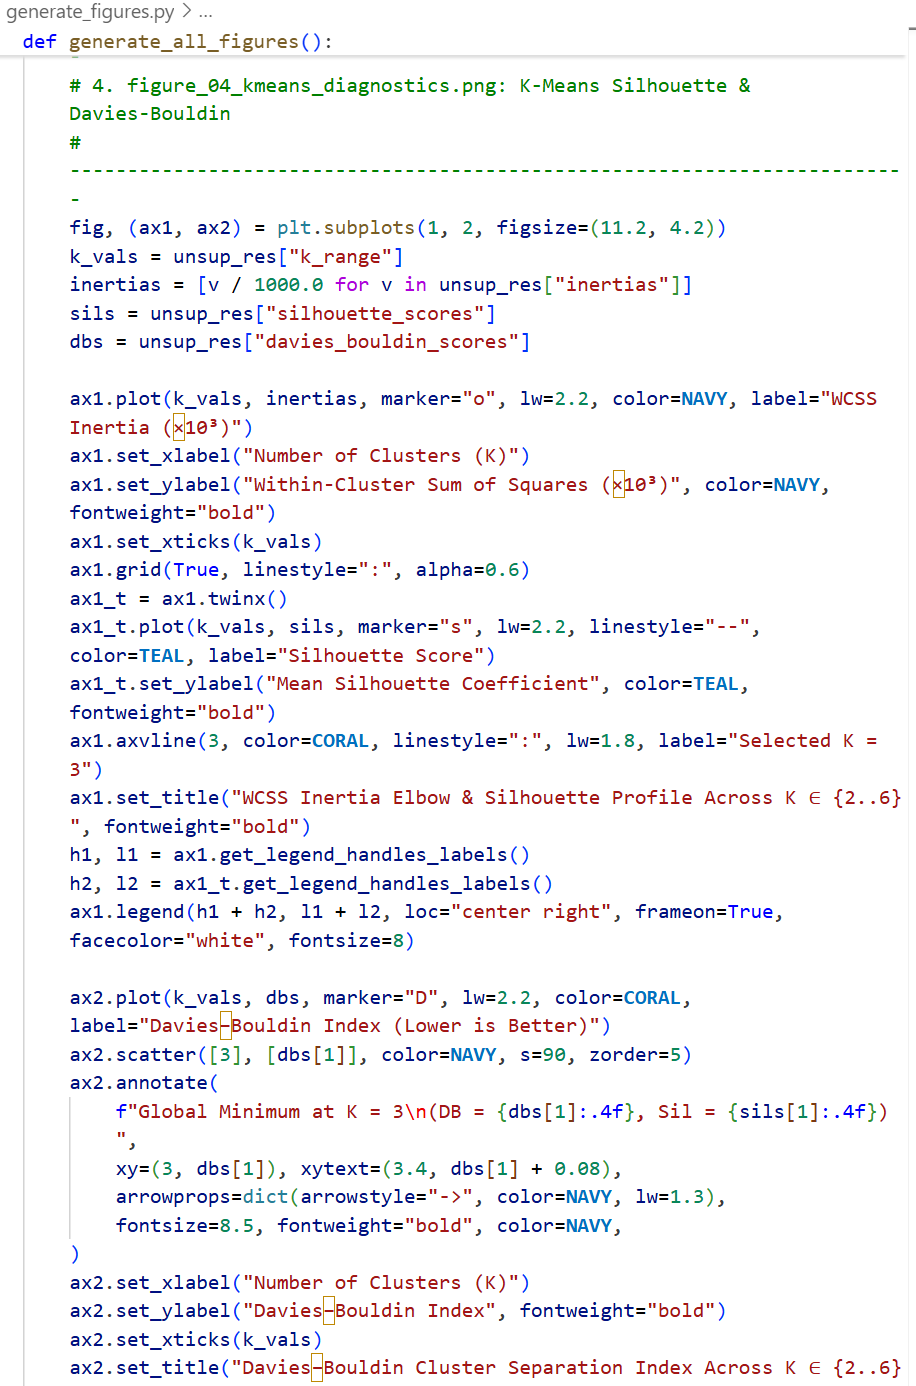
\includegraphics[width=\textwidth,height=0.33\textheight,keepaspectratio]{../figures/generate_figures7.png}
\end{minipage}\hfill
\begin{minipage}[t]{0.475\textwidth}\vspace{0pt}
    \centering
    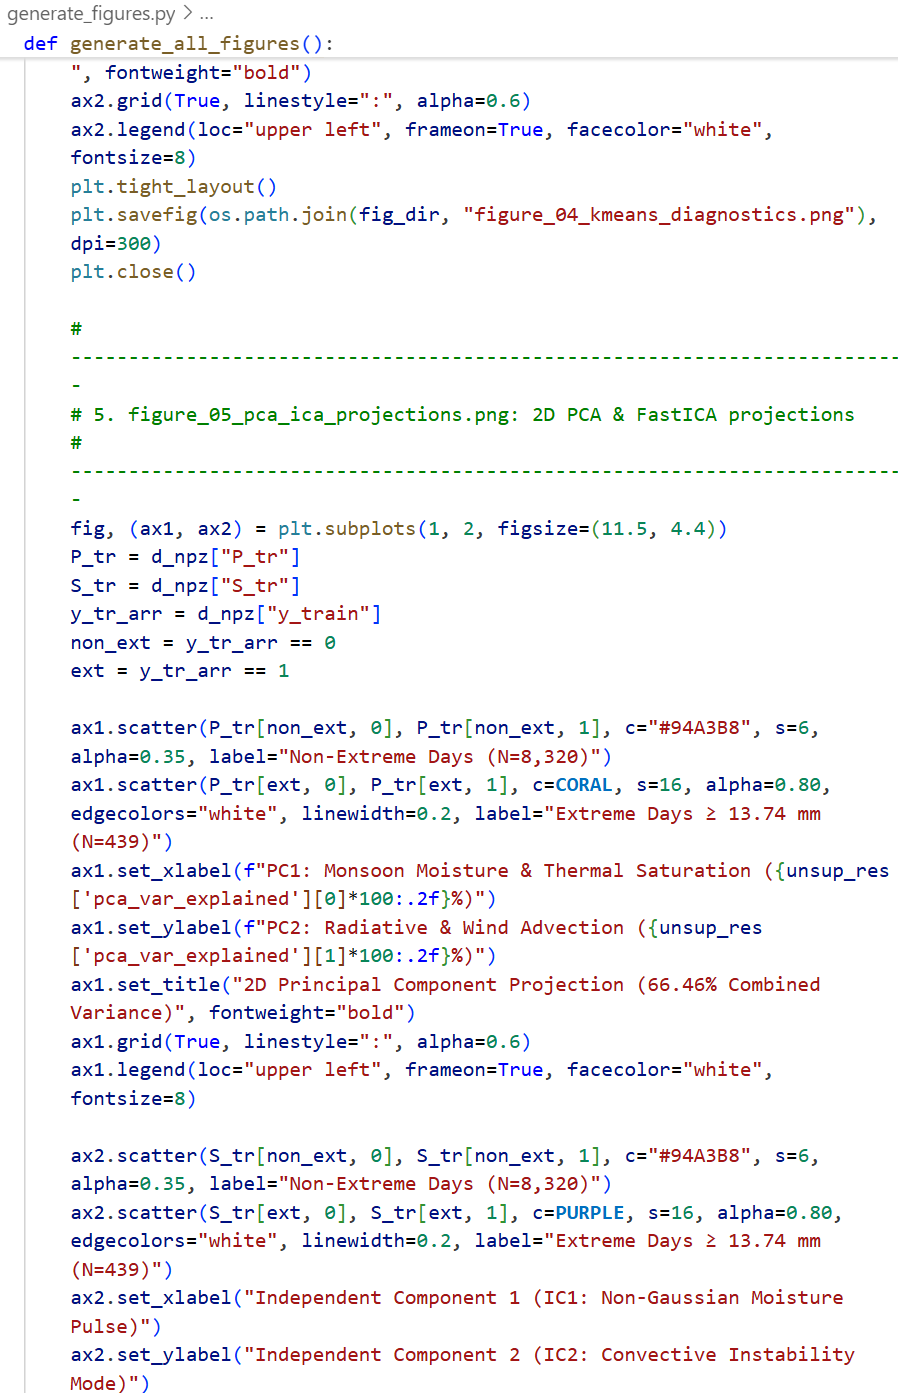
\includegraphics[width=\textwidth,height=0.33\textheight,keepaspectratio]{../figures/generate_figures8.png}
\end{minipage}
\vspace{2.8em}
\noindent
\begin{minipage}[t]{0.475\textwidth}\vspace{0pt}
    \centering
    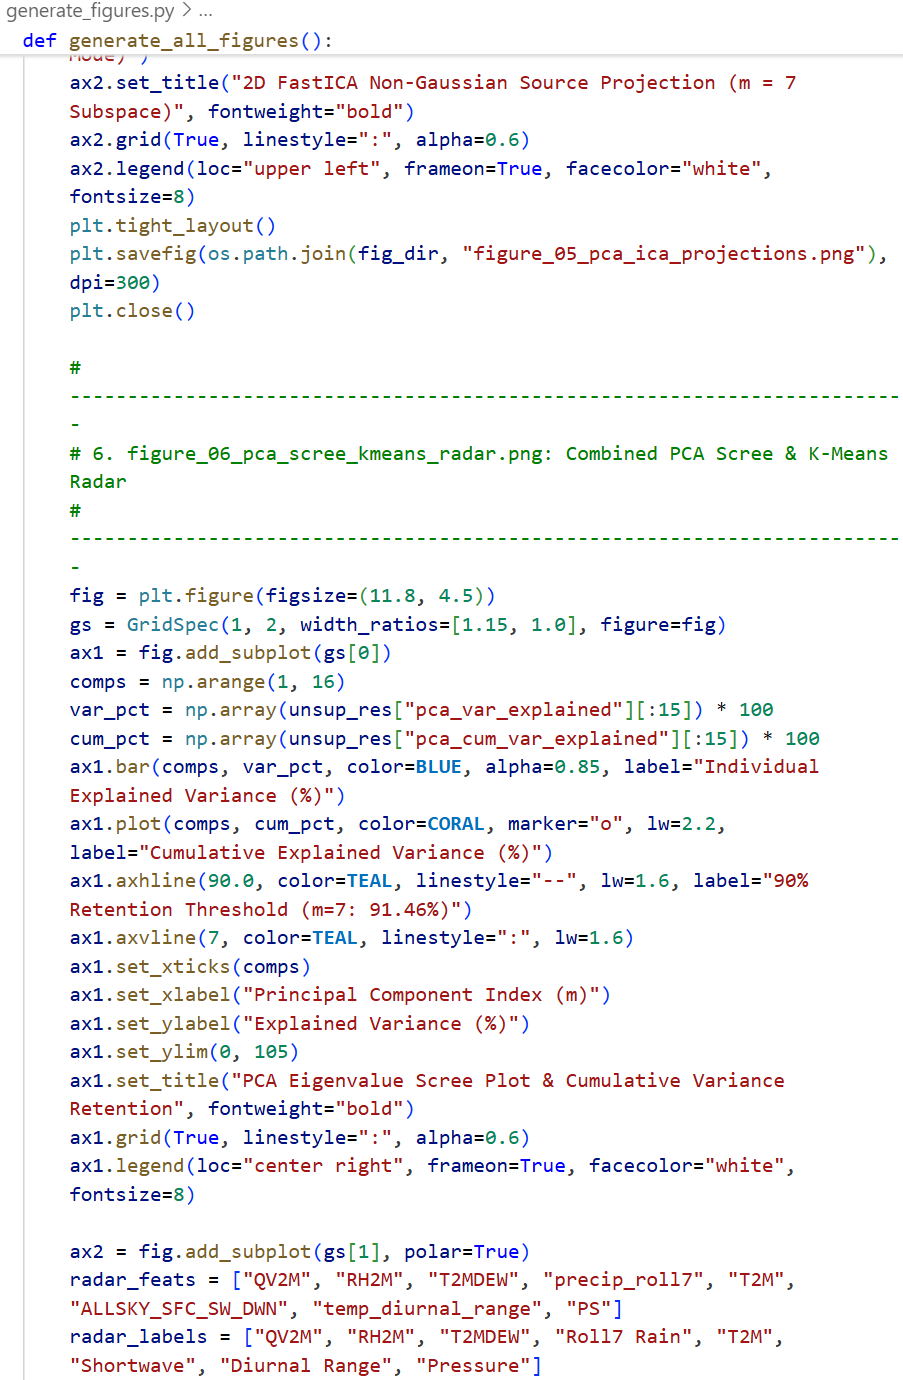
\includegraphics[width=\textwidth,height=0.33\textheight,keepaspectratio]{../figures/generate_figures9.png}
\end{minipage}\hfill
\begin{minipage}[t]{0.475\textwidth}\vspace{0pt}
    \centering
    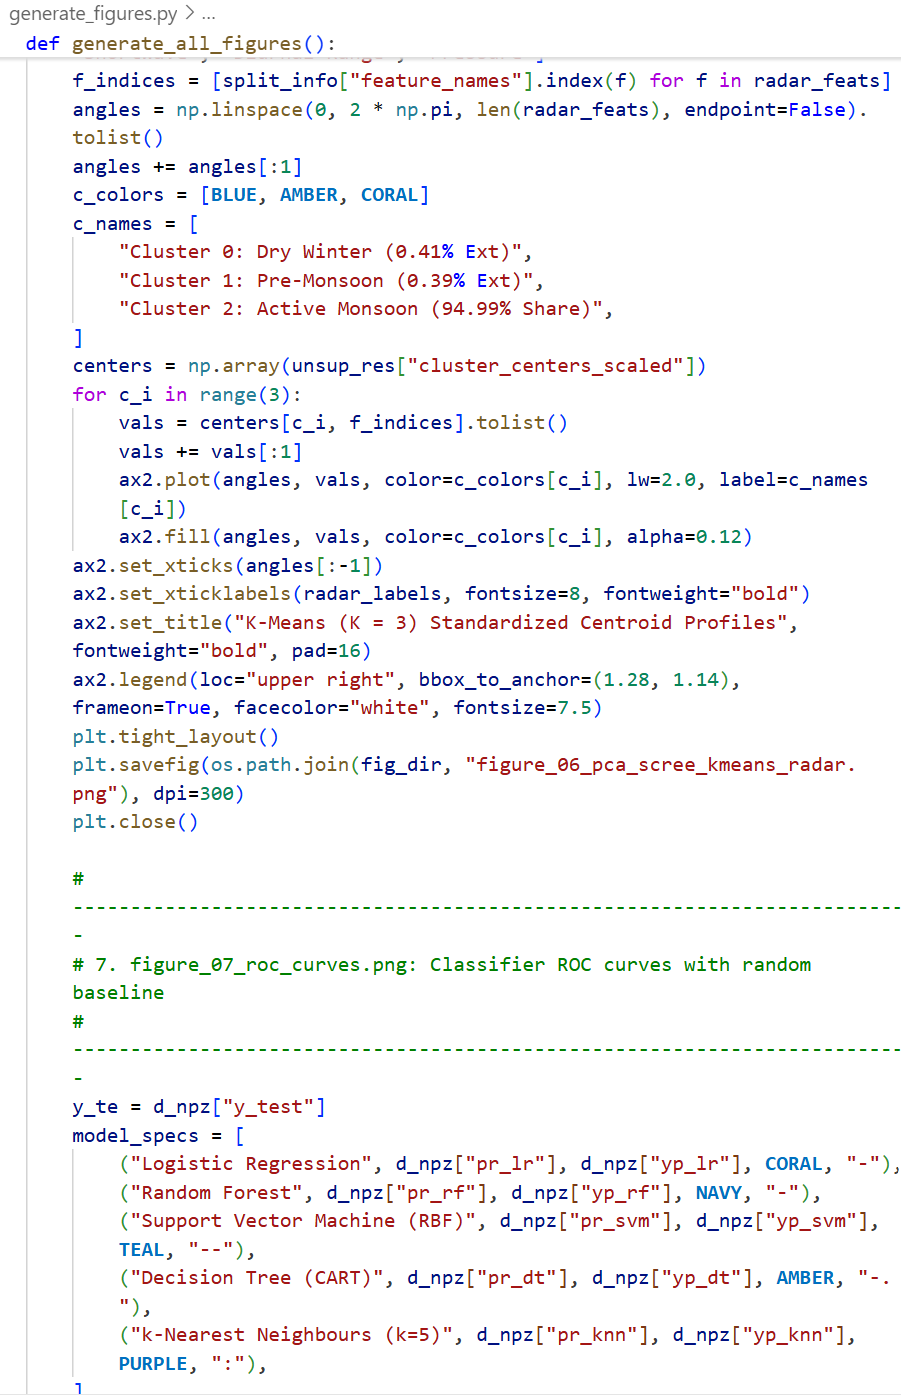
\includegraphics[width=\textwidth,height=0.33\textheight,keepaspectratio]{../figures/generate_figures10.png}
\end{minipage}
\clearpage
\noindent
\begin{minipage}[t]{0.475\textwidth}\vspace{0pt}
    \centering
    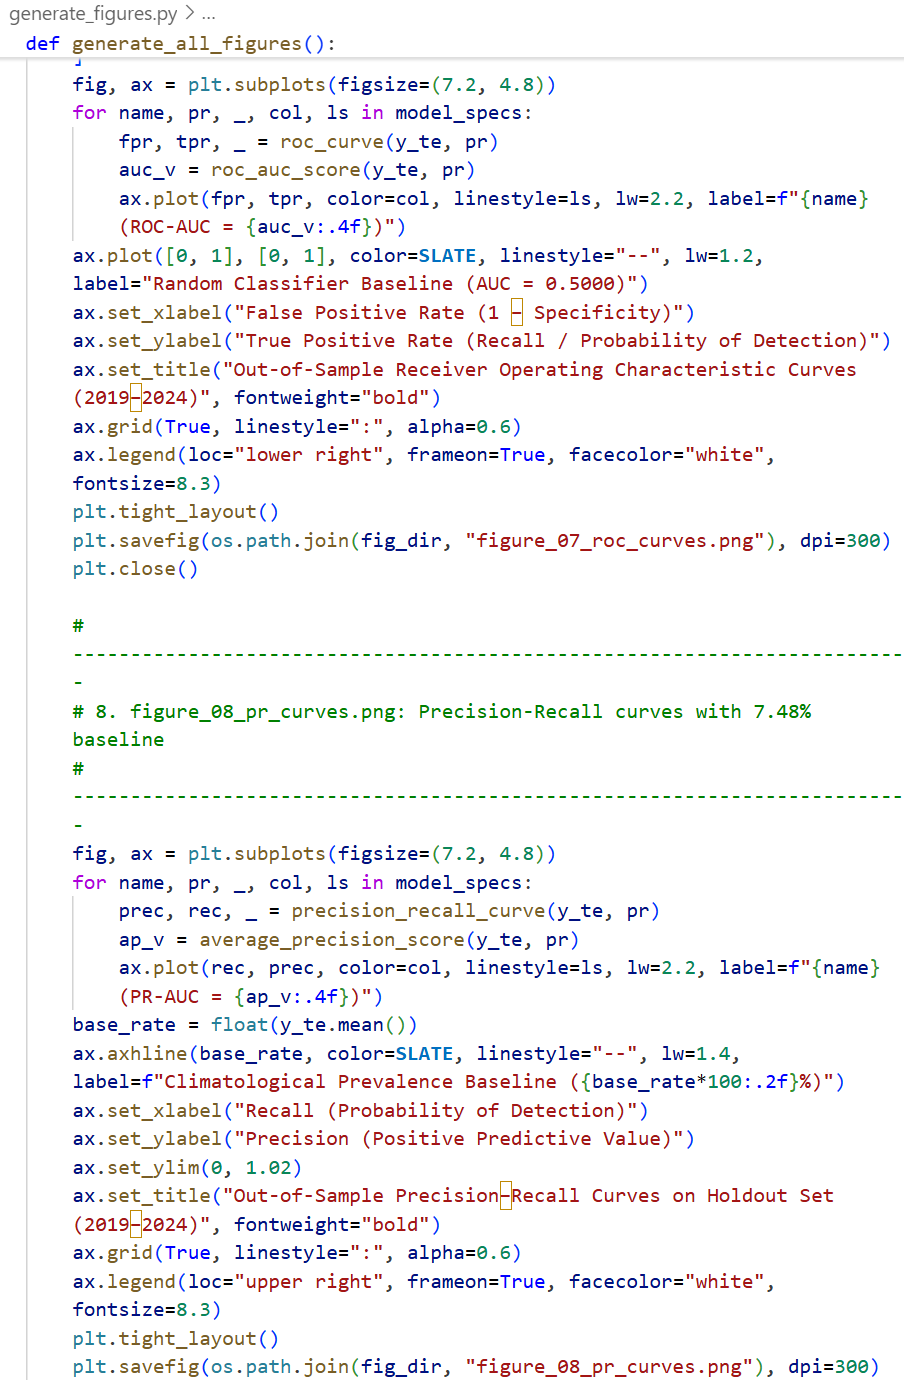
\includegraphics[width=\textwidth,height=0.33\textheight,keepaspectratio]{../figures/generate_figures11.png}
\end{minipage}\hfill
\begin{minipage}[t]{0.475\textwidth}\vspace{0pt}
    \centering
    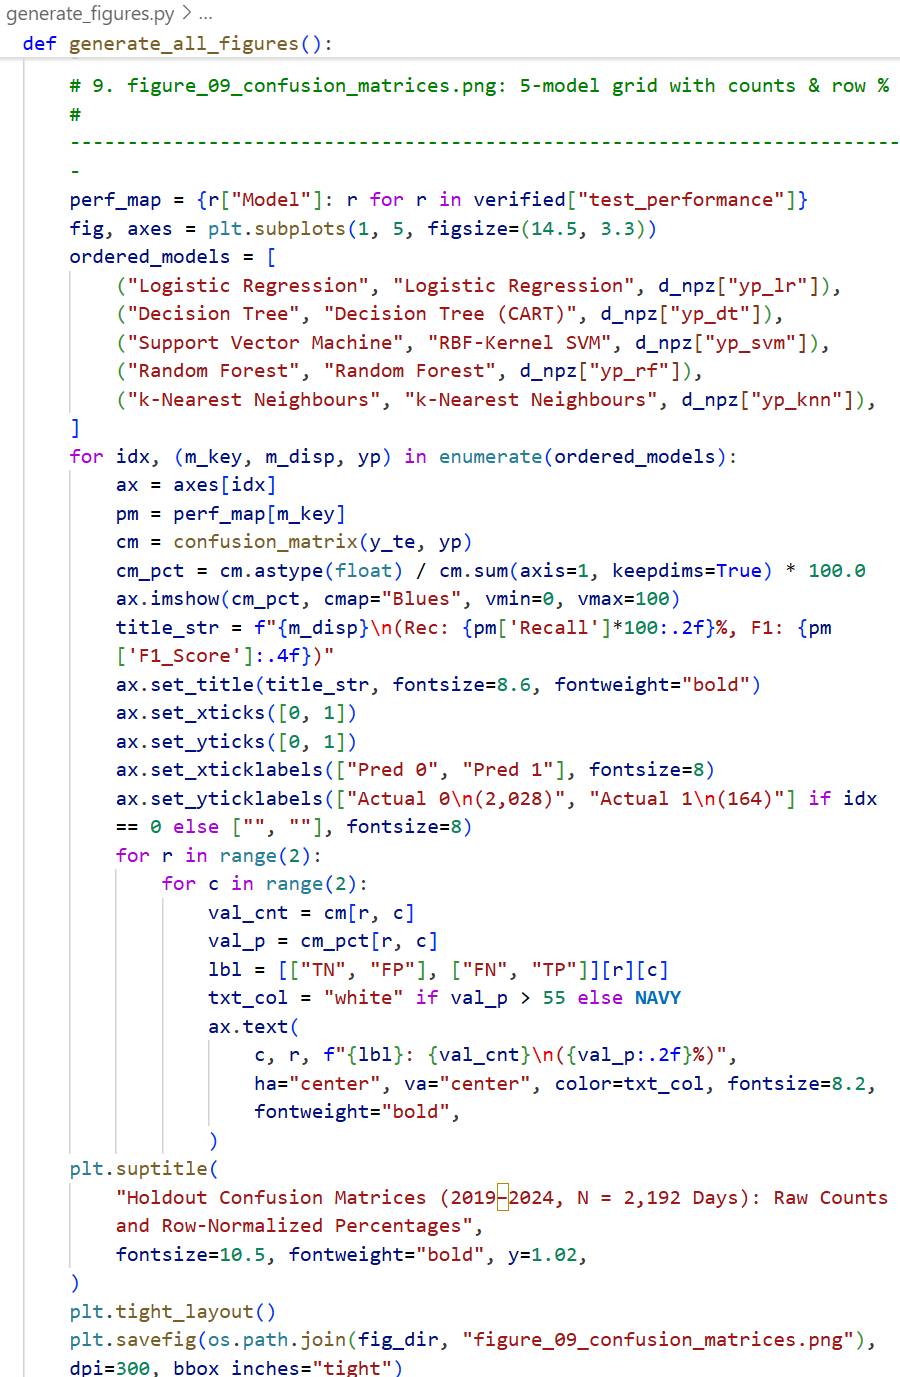
\includegraphics[width=\textwidth,height=0.33\textheight,keepaspectratio]{../figures/generate_figures12.png}
\end{minipage}
\vspace{2.8em}
\noindent
\begin{minipage}[t]{0.475\textwidth}\vspace{0pt}
    \centering
    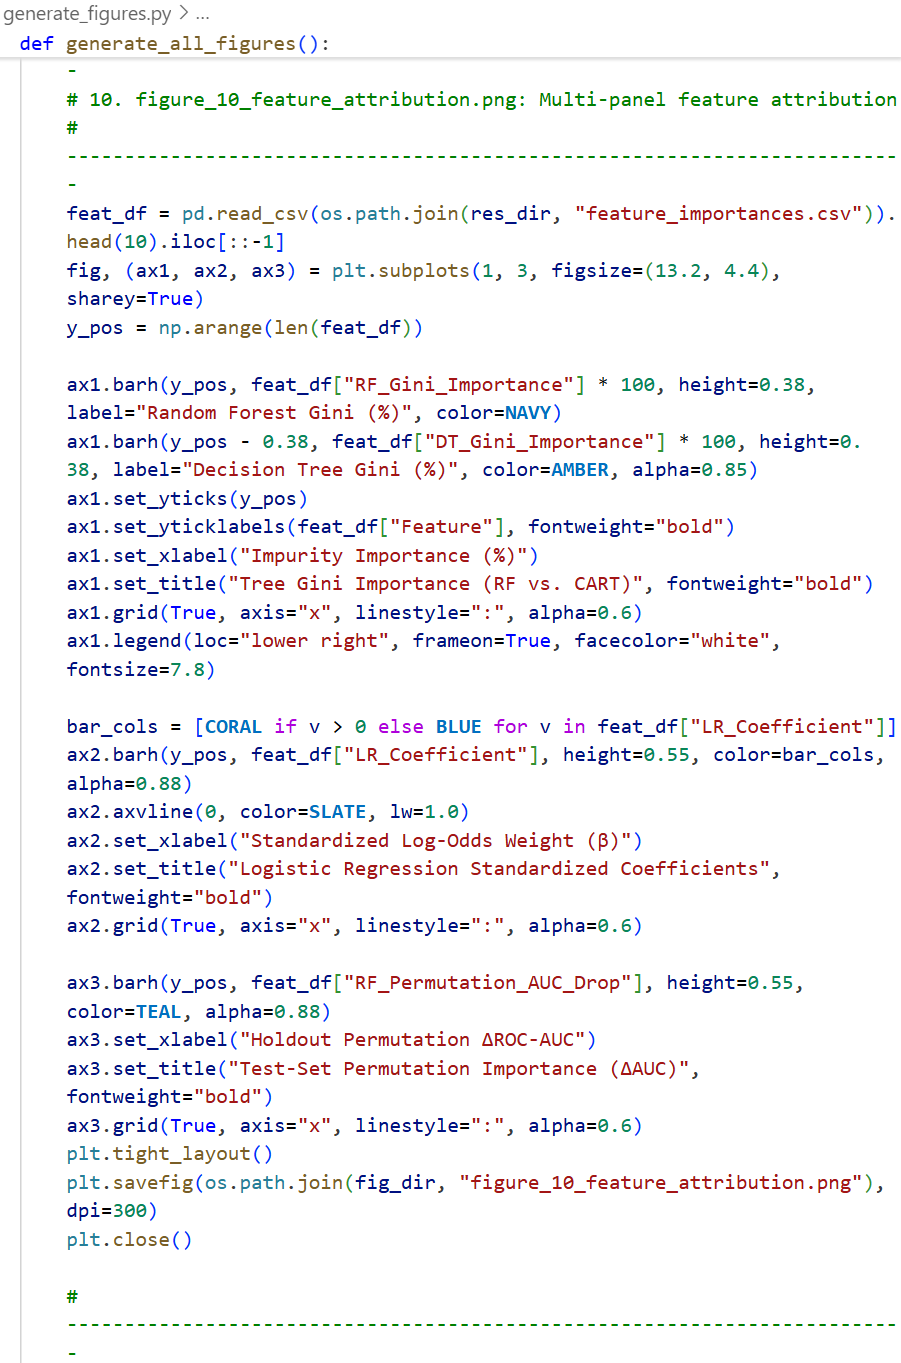
\includegraphics[width=\textwidth,height=0.33\textheight,keepaspectratio]{../figures/generate_figures13.png}
\end{minipage}\hfill
\begin{minipage}[t]{0.475\textwidth}\vspace{0pt}
    \centering
    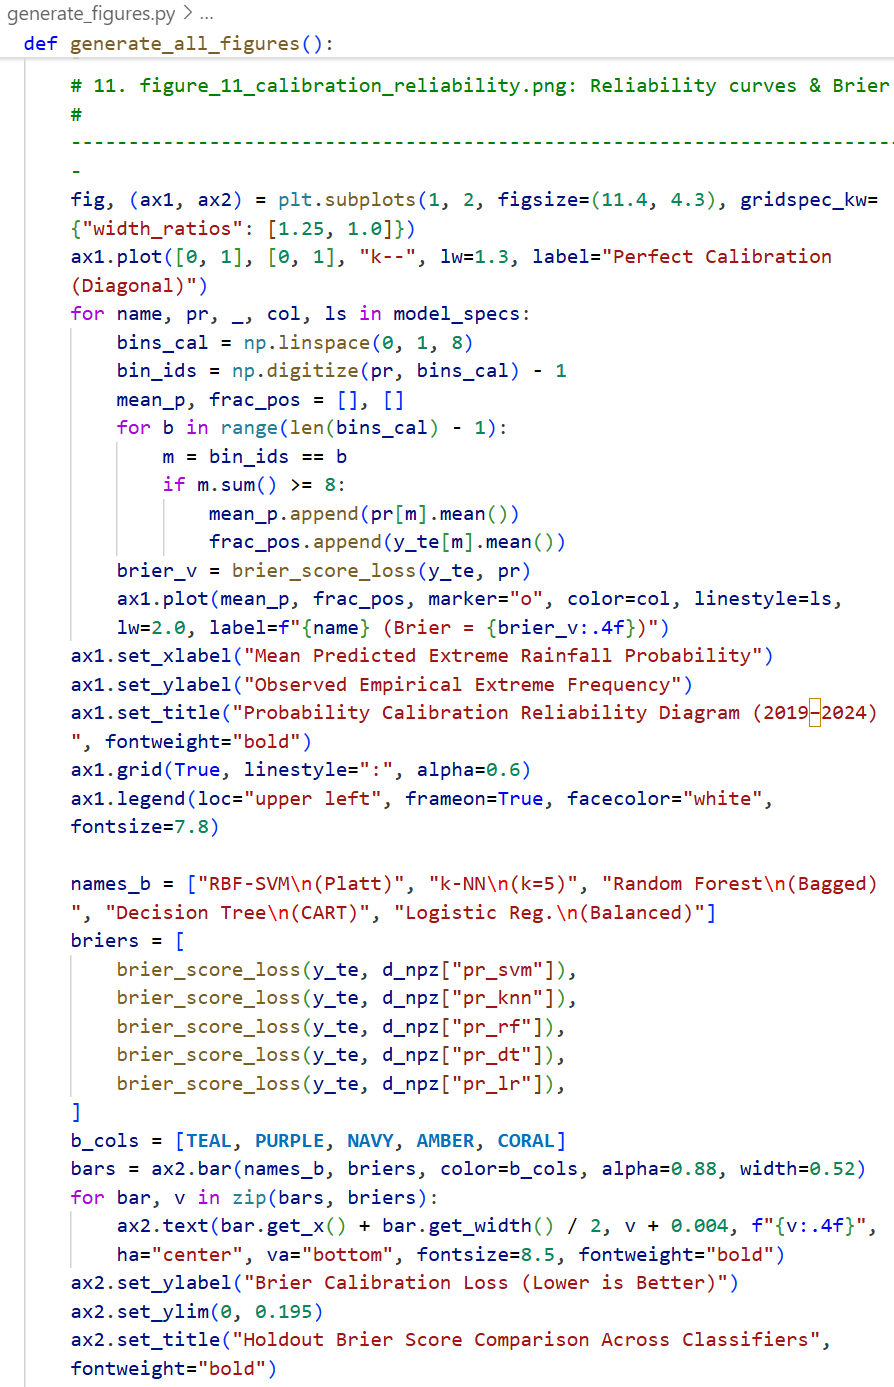
\includegraphics[width=\textwidth,height=0.33\textheight,keepaspectratio]{../figures/generate_figures14.png}
\end{minipage}
\clearpage
\noindent
\begin{minipage}[t]{0.475\textwidth}\vspace{0pt}
    \centering
    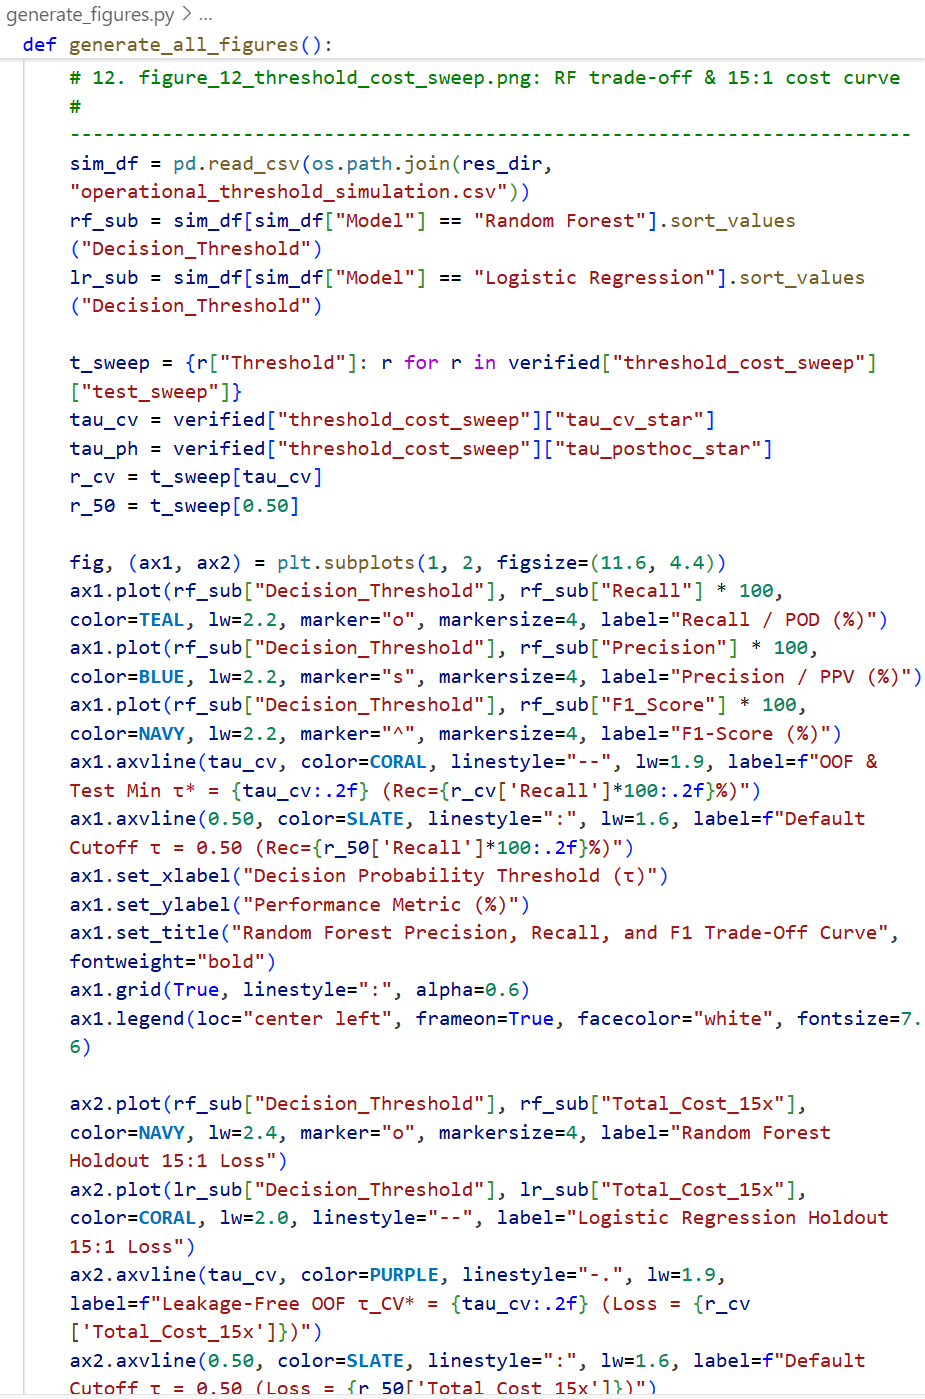
\includegraphics[width=\textwidth,height=0.33\textheight,keepaspectratio]{../figures/generate_figures15.png}
\end{minipage}\hfill
\begin{minipage}[t]{0.475\textwidth}\vspace{0pt}
    \centering
    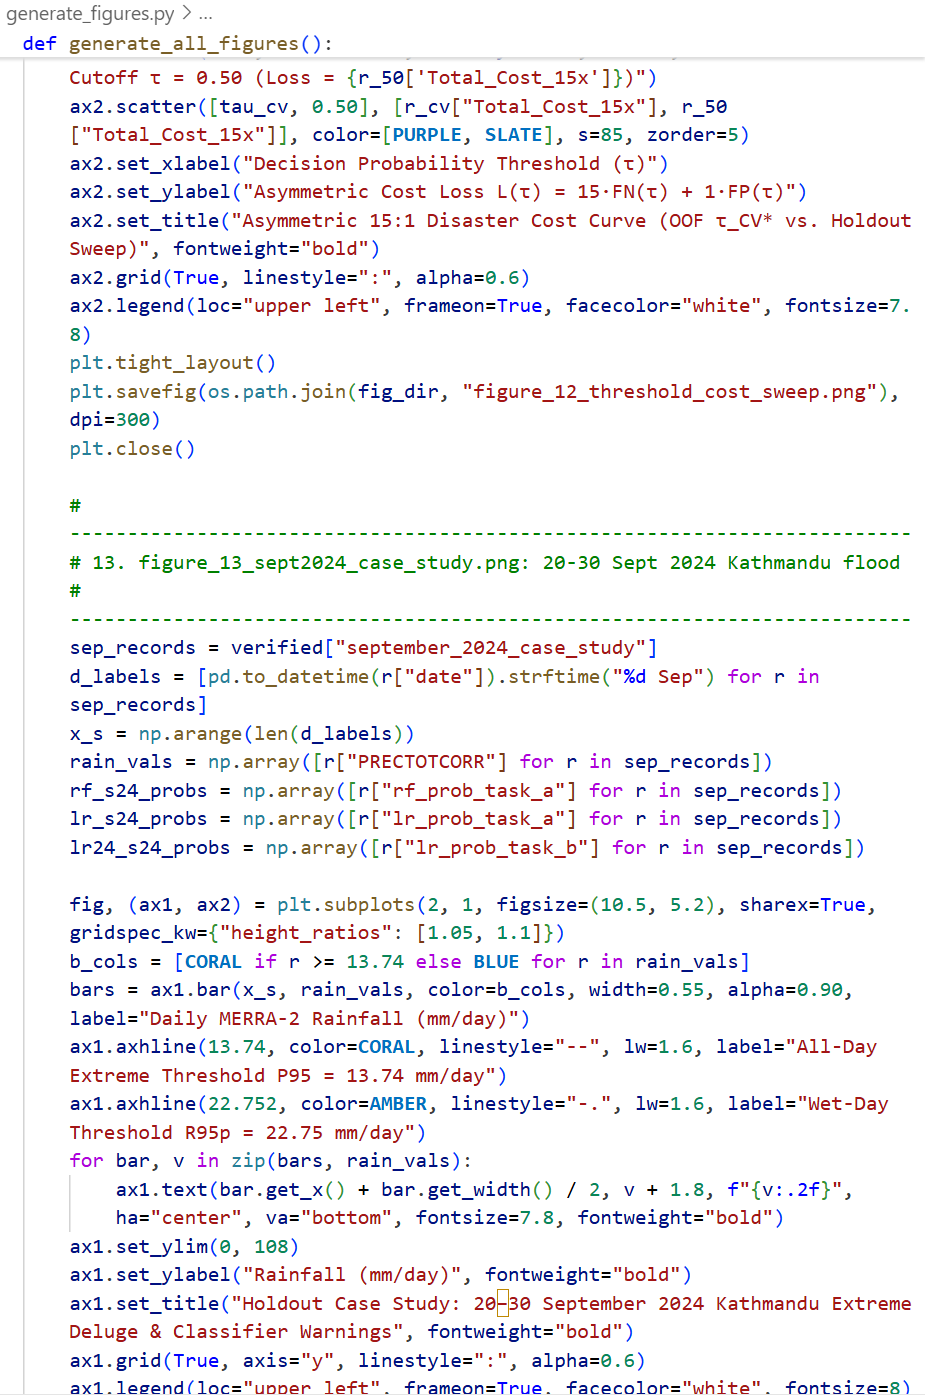
\includegraphics[width=\textwidth,height=0.33\textheight,keepaspectratio]{../figures/generate_figures16.png}
\end{minipage}
\vspace{2.8em}
\noindent
\begin{minipage}[t]{0.475\textwidth}\vspace{0pt}
    \centering
    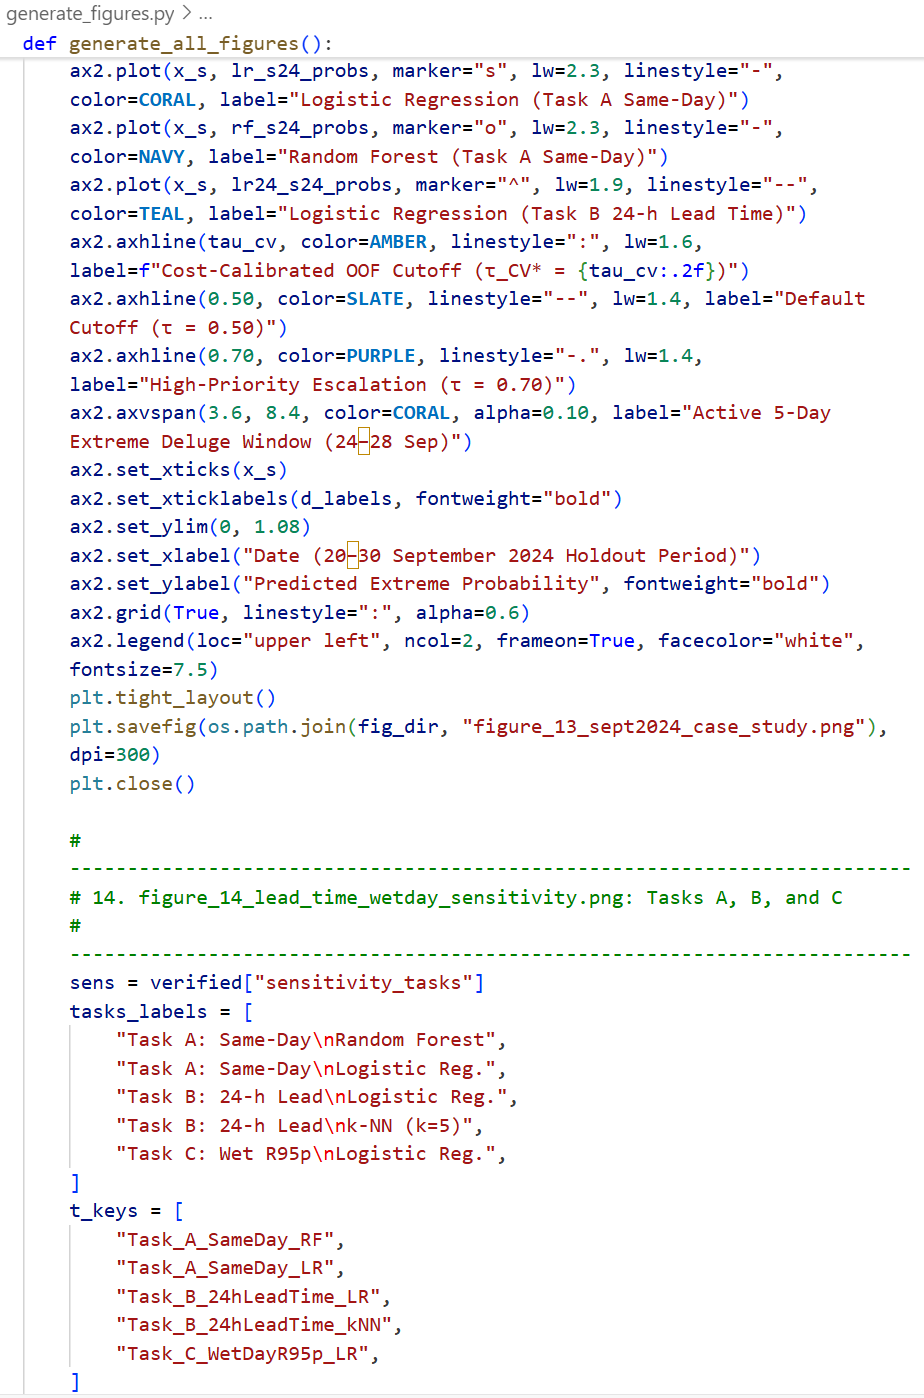
\includegraphics[width=\textwidth,height=0.33\textheight,keepaspectratio]{../figures/generate_figures17.png}
\end{minipage}\hfill
\begin{minipage}[t]{0.475\textwidth}\vspace{0pt}
    \centering
    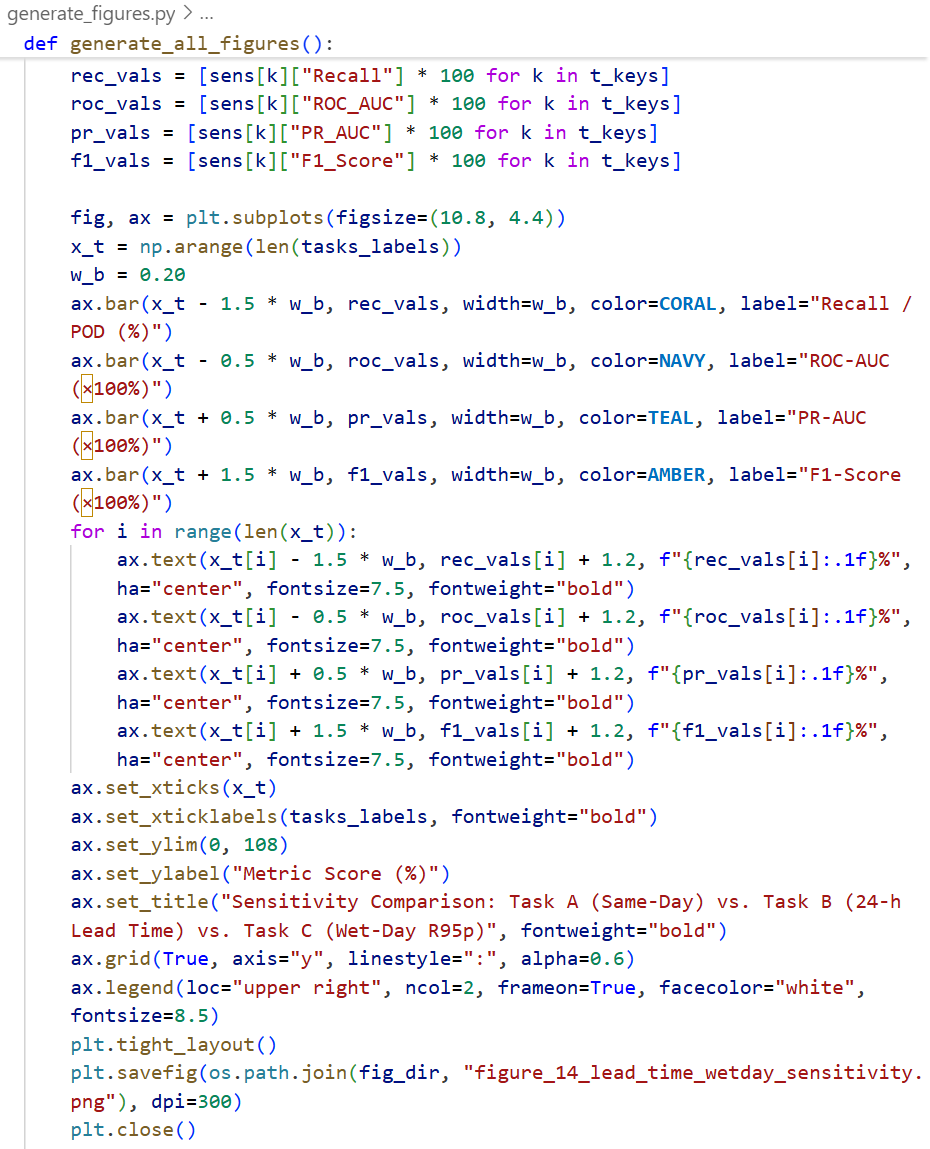
\includegraphics[width=\textwidth,height=0.33\textheight,keepaspectratio]{../figures/generate_figures18.png}
\end{minipage}
\clearpage

\subsection*{D.\quad OPERATIONAL DASHBOARD PROTOTYPE}
\vspace{0.6em}

\noindent
\begin{minipage}[t]{0.475\textwidth}\vspace{0pt}
    \centering
    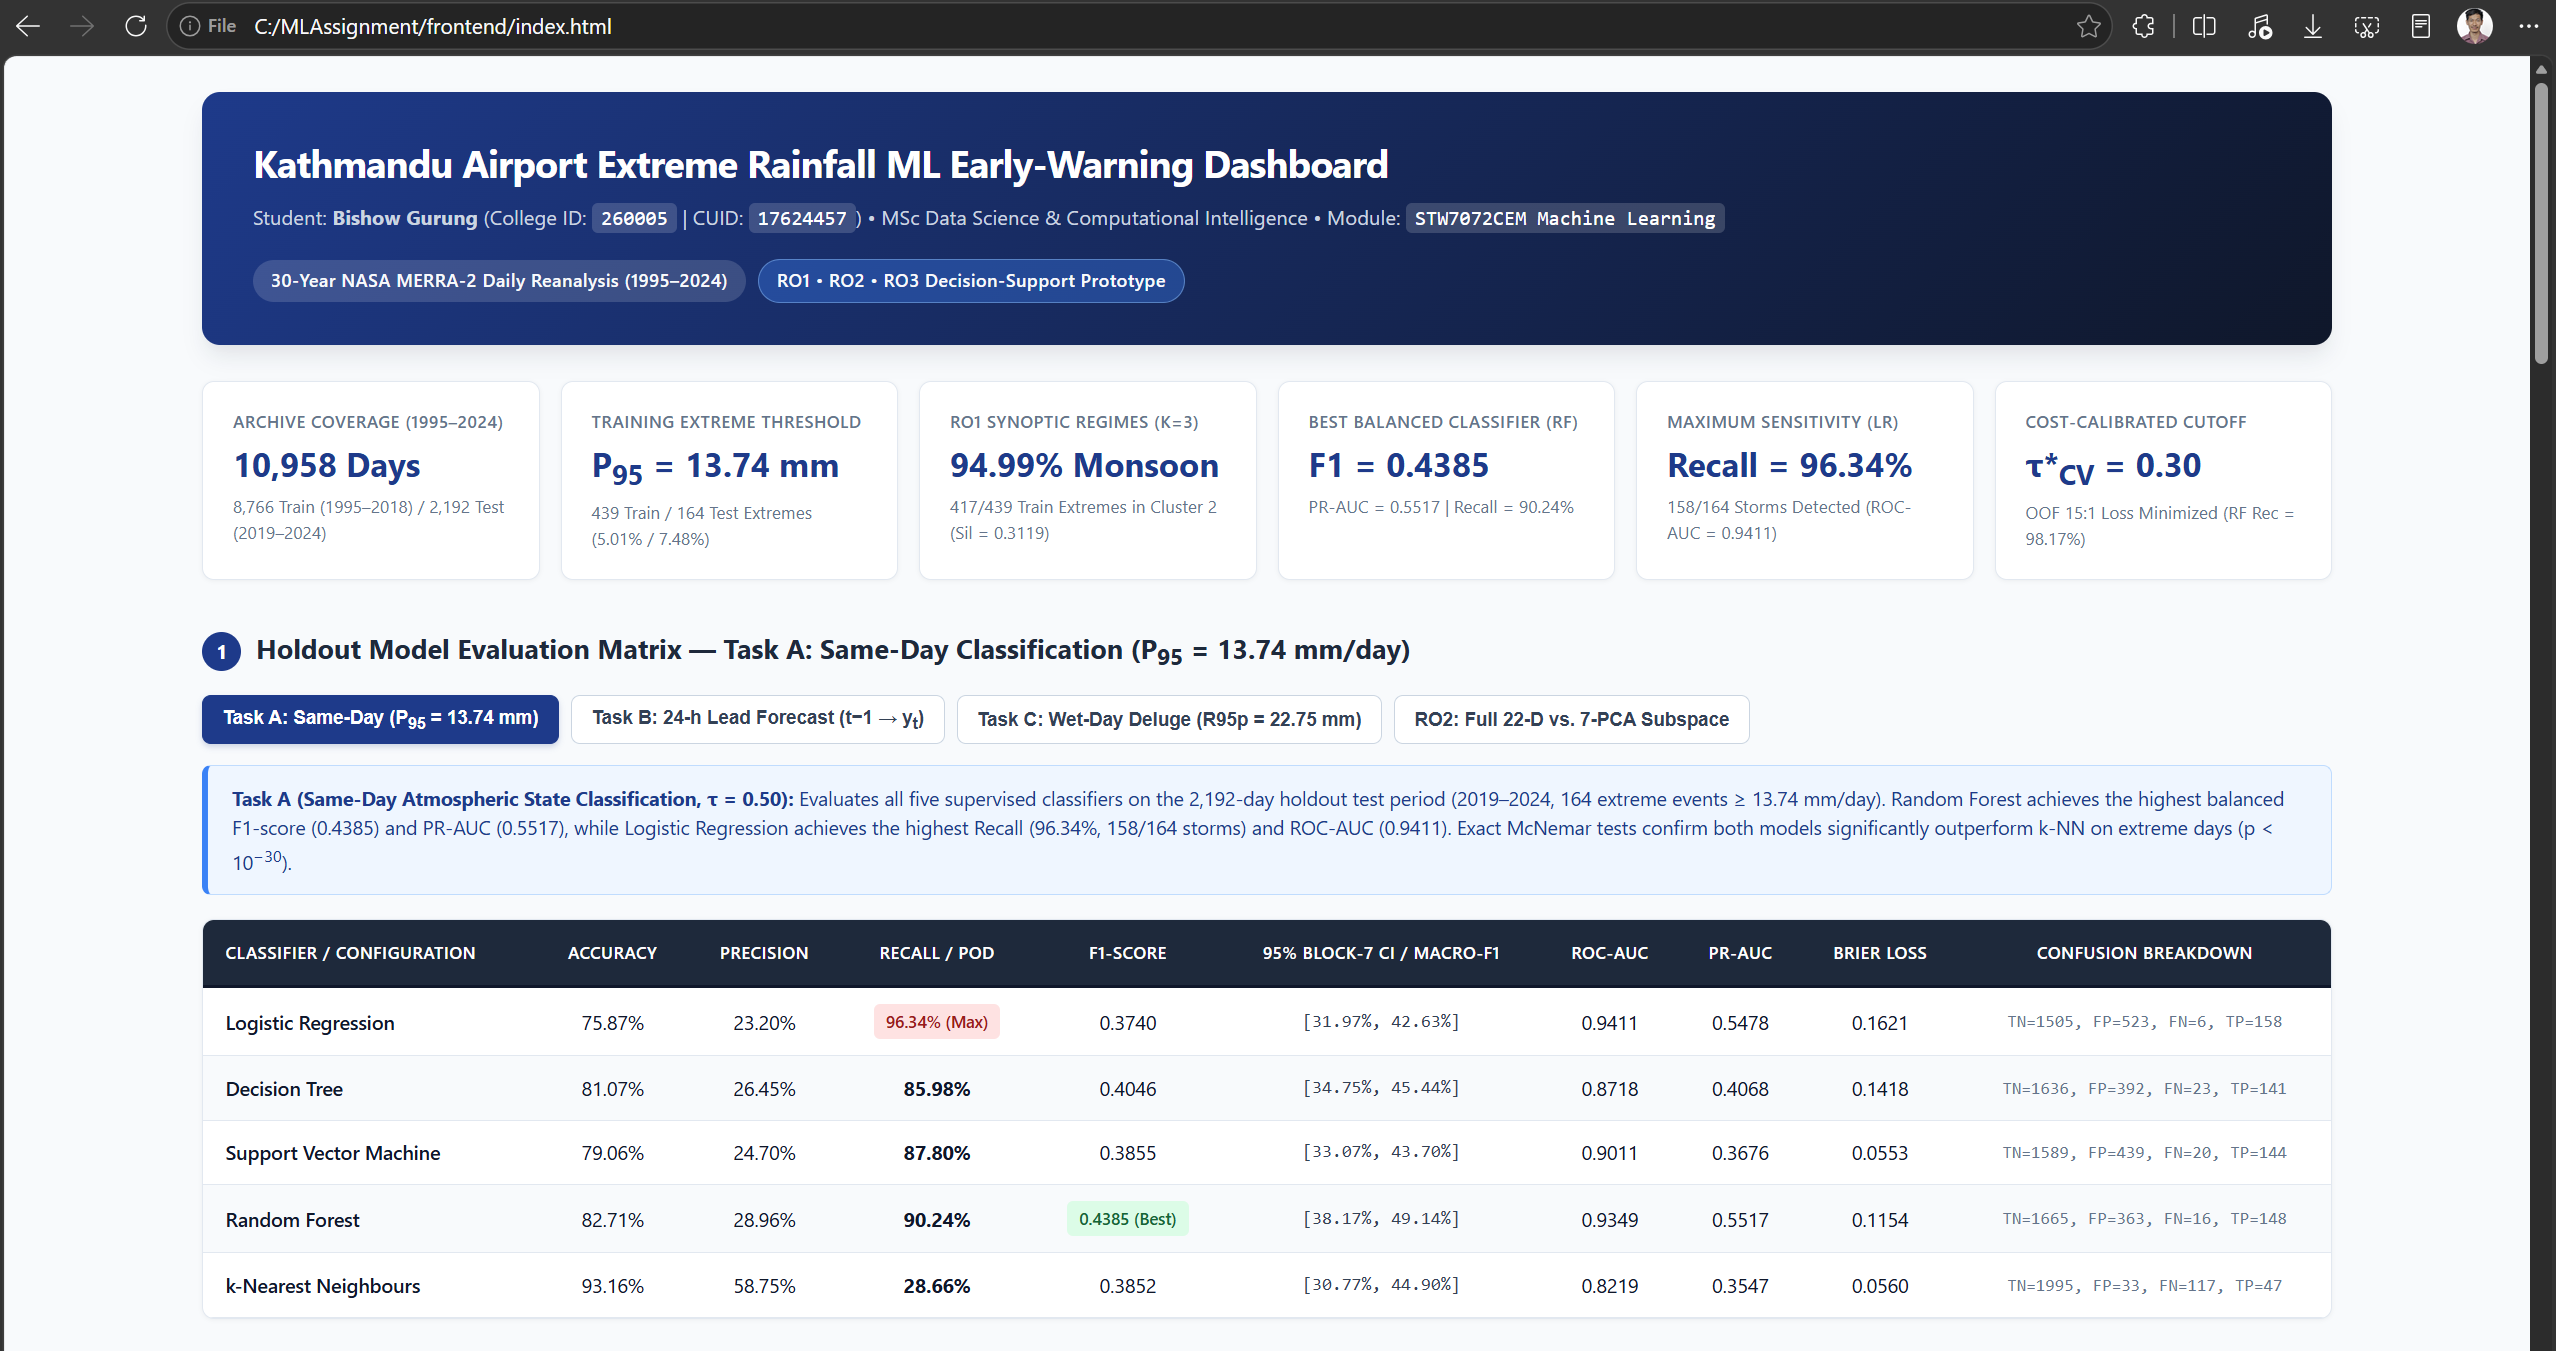
\includegraphics[width=\textwidth,height=0.33\textheight,keepaspectratio]{../figures/dashboard1.png}
\end{minipage}\hfill
\begin{minipage}[t]{0.475\textwidth}\vspace{0pt}
    \centering
    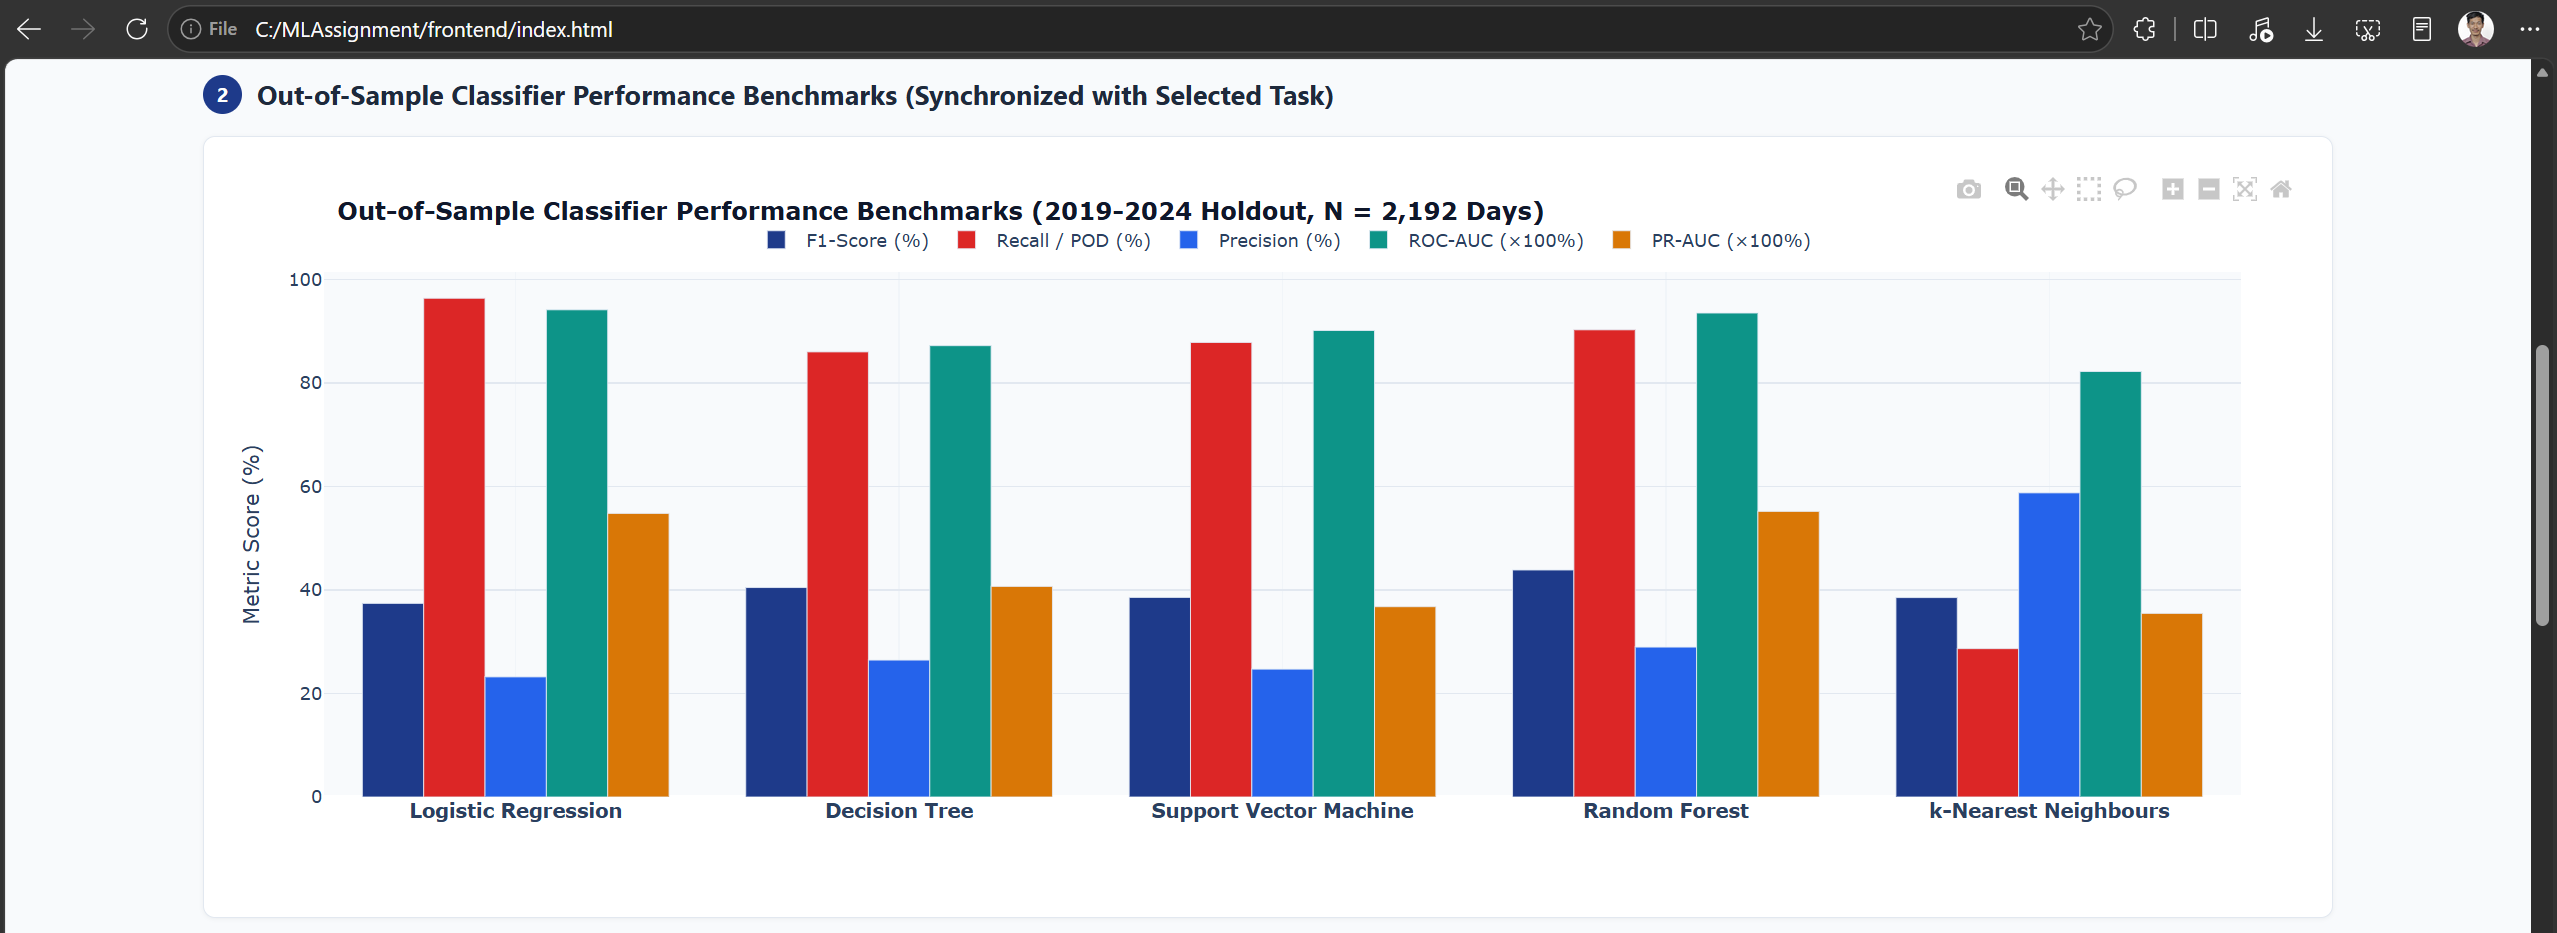
\includegraphics[width=\textwidth,height=0.33\textheight,keepaspectratio]{../figures/dashboard2.png}
\end{minipage}
\vspace{2.8em}
\noindent
\begin{minipage}[t]{0.475\textwidth}\vspace{0pt}
    \centering
    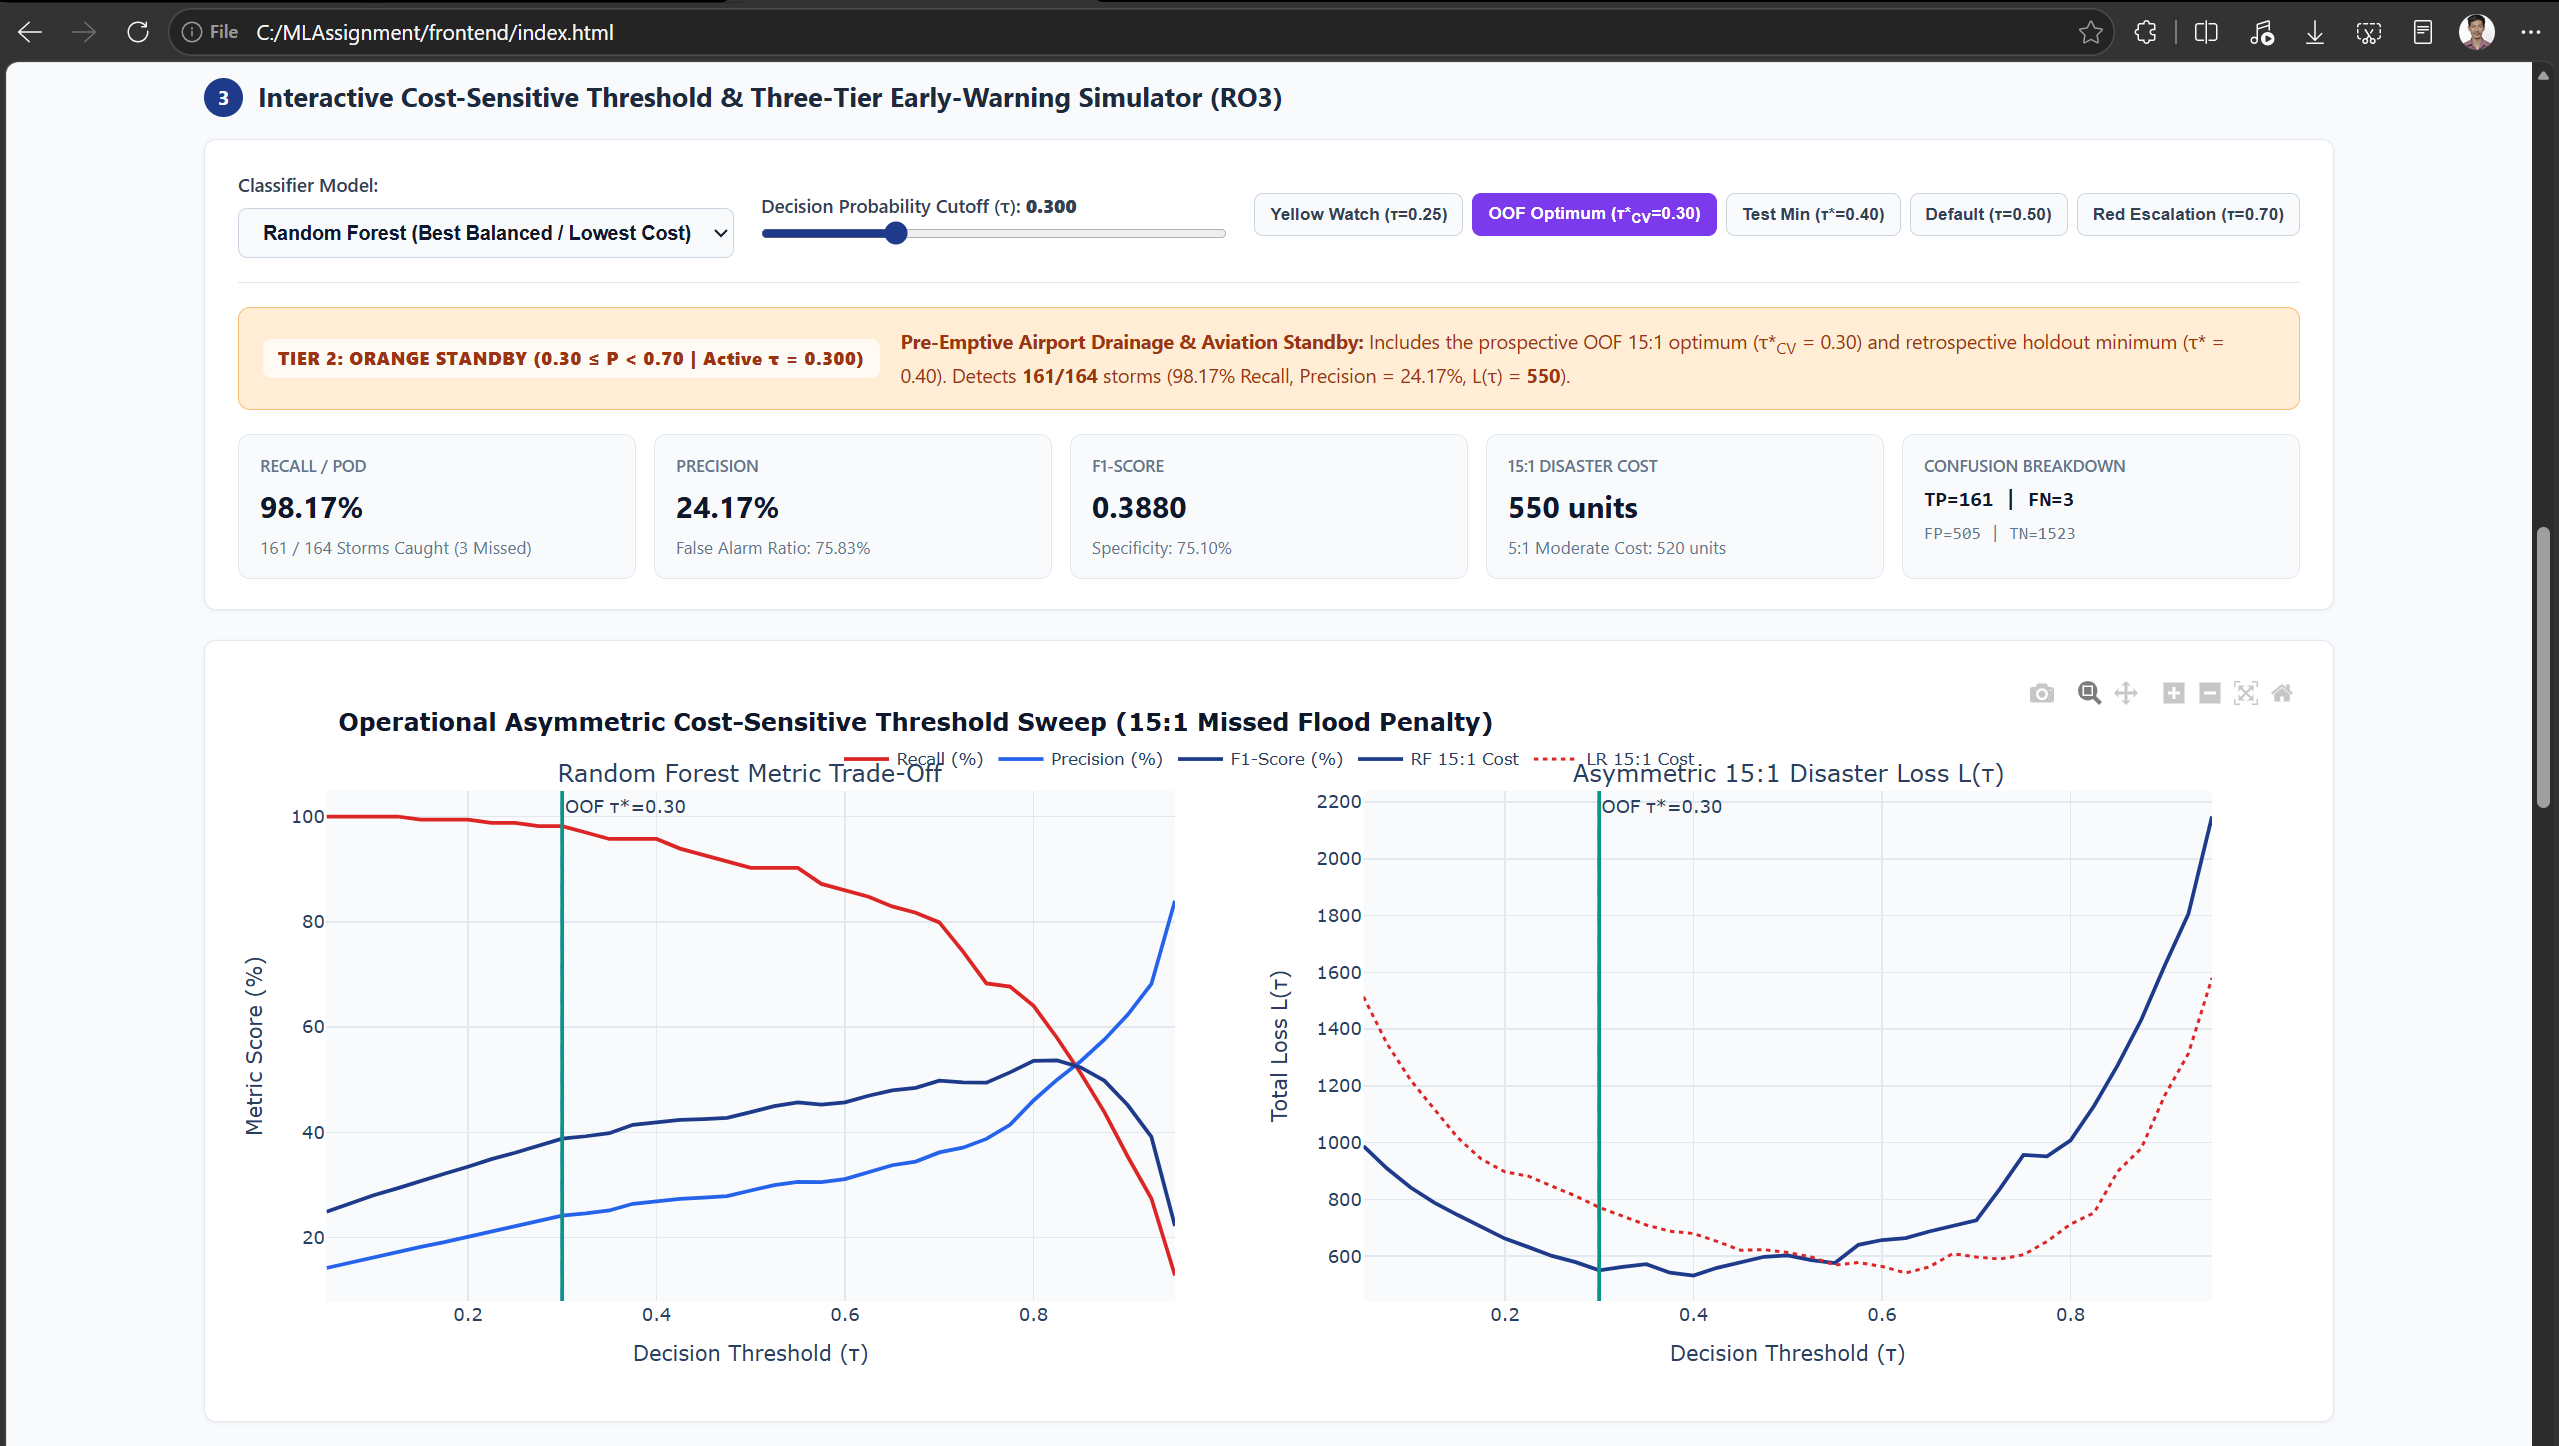
\includegraphics[width=\textwidth,height=0.33\textheight,keepaspectratio]{../figures/dashboard3.png}
\end{minipage}\hfill
\begin{minipage}[t]{0.475\textwidth}\vspace{0pt}
    \centering
    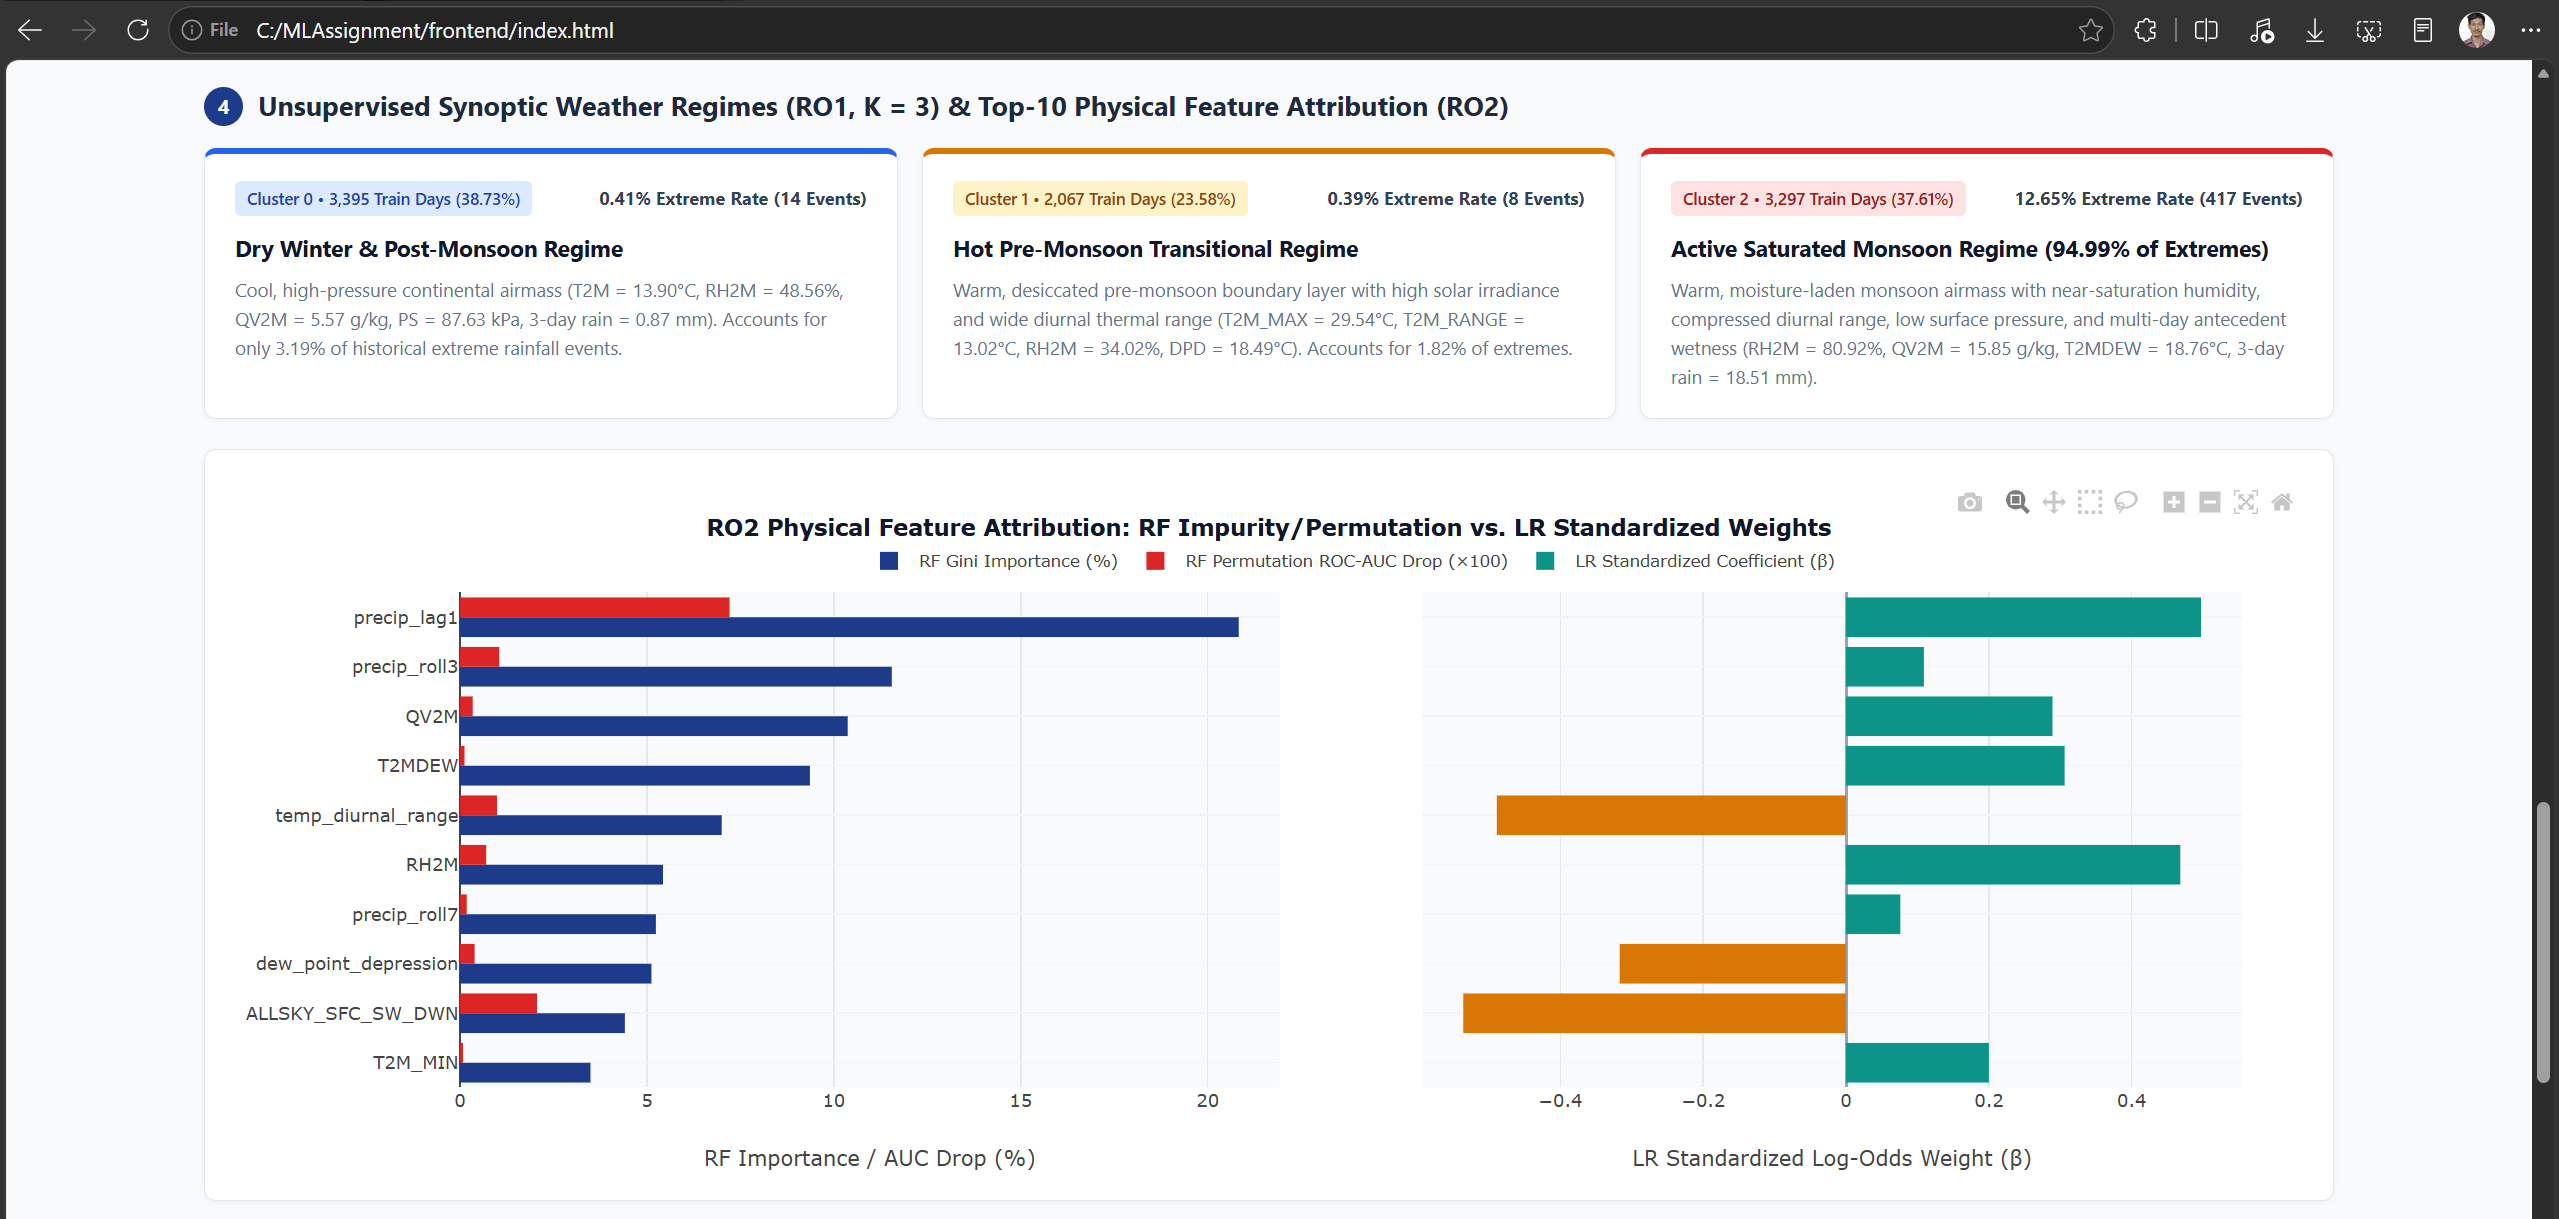
\includegraphics[width=\textwidth,height=0.33\textheight,keepaspectratio]{../figures/dashboard4.png}
\end{minipage}
\clearpage
\noindent
\begin{minipage}[t]{0.475\textwidth}\vspace{0pt}
    \centering
    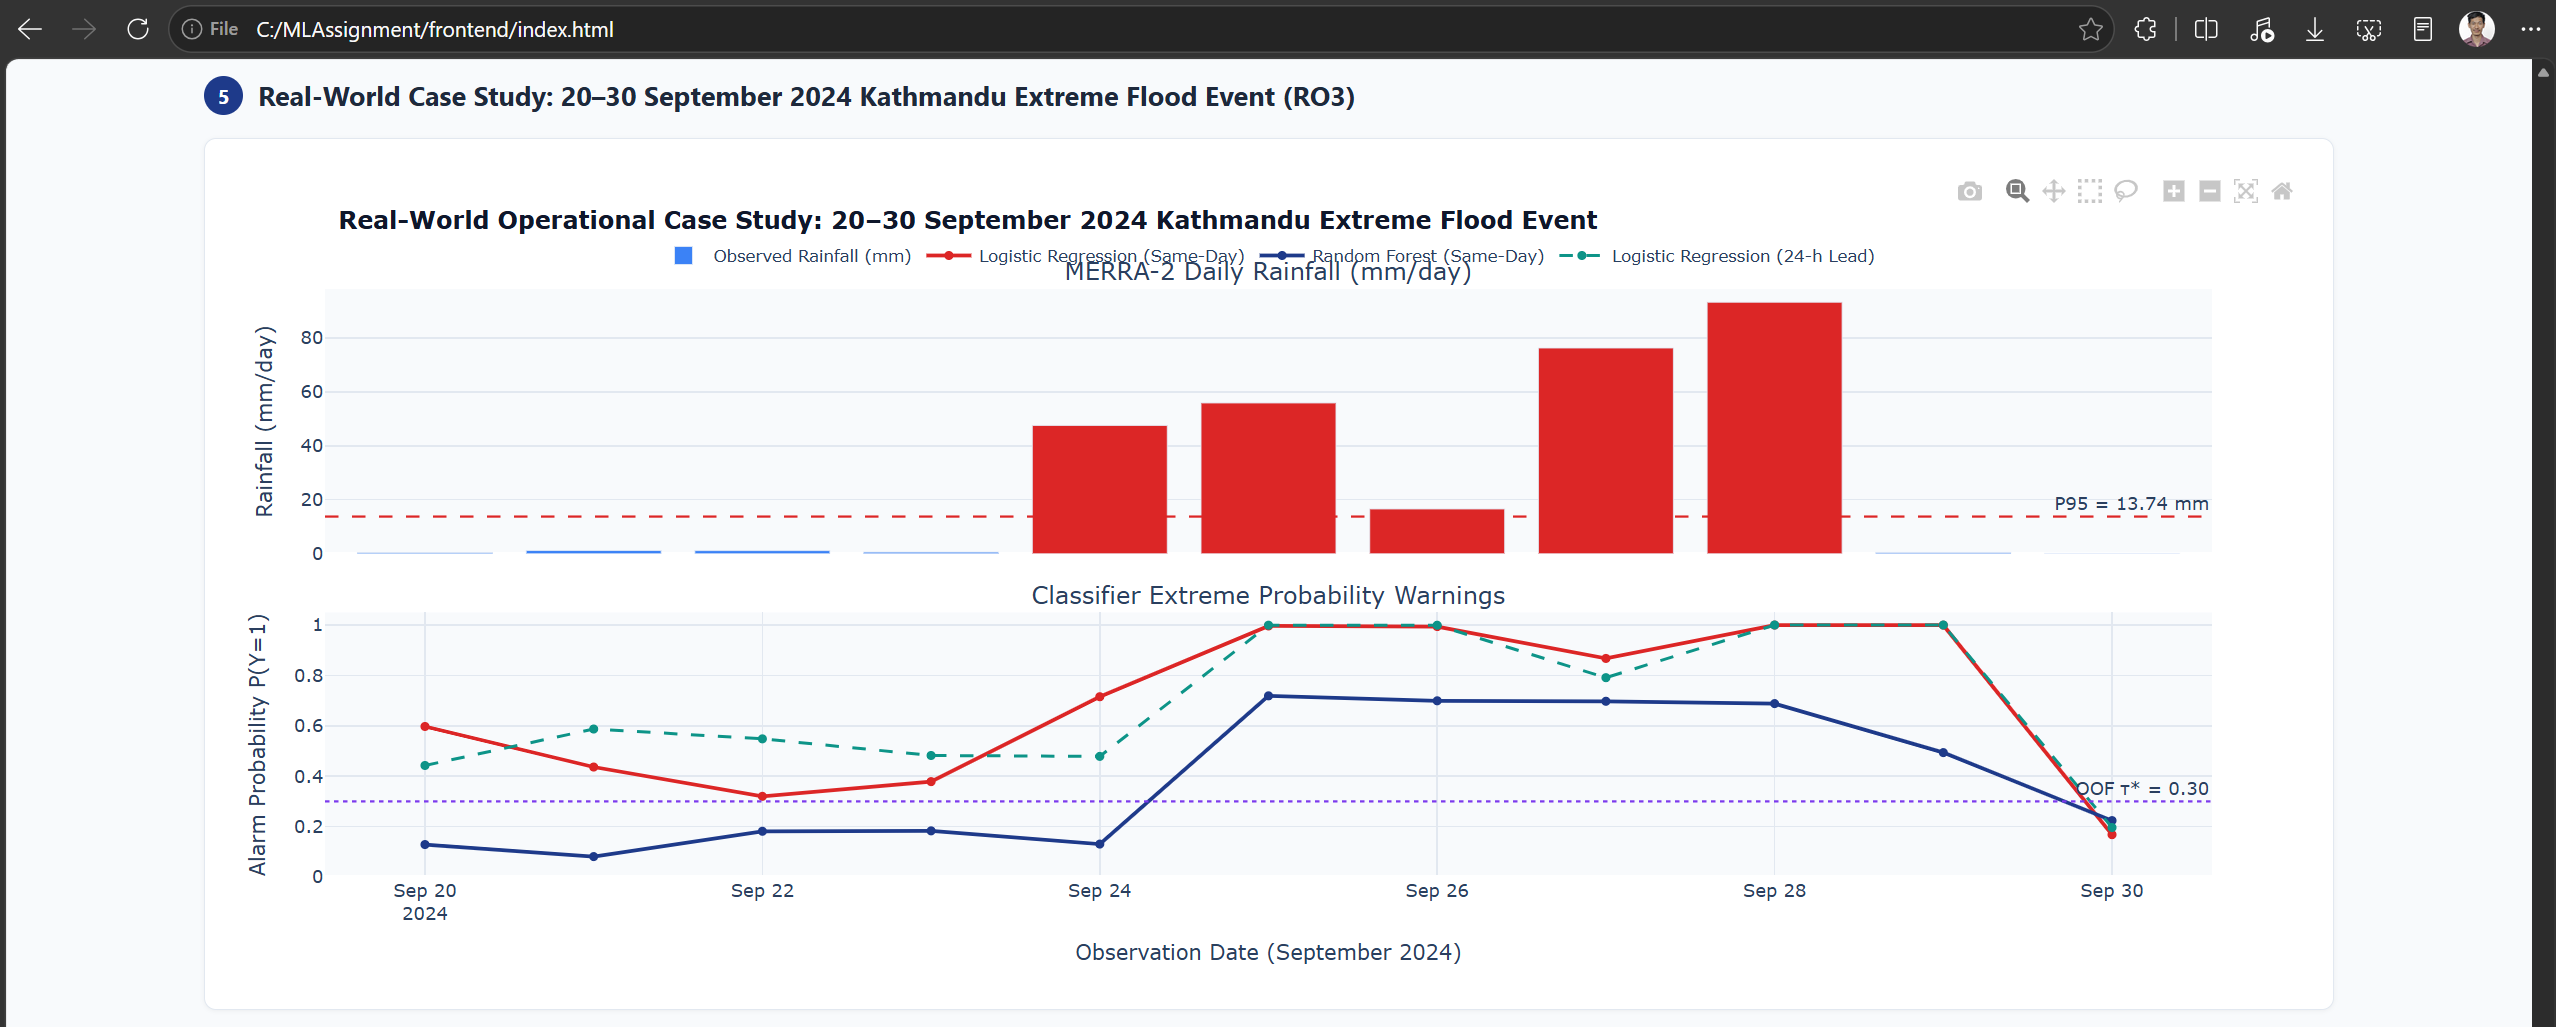
\includegraphics[width=\textwidth,height=0.33\textheight,keepaspectratio]{../figures/dashboard5.png}
\end{minipage}\hfill
\begin{minipage}[t]{0.475\textwidth}\vspace{0pt}
    \centering
    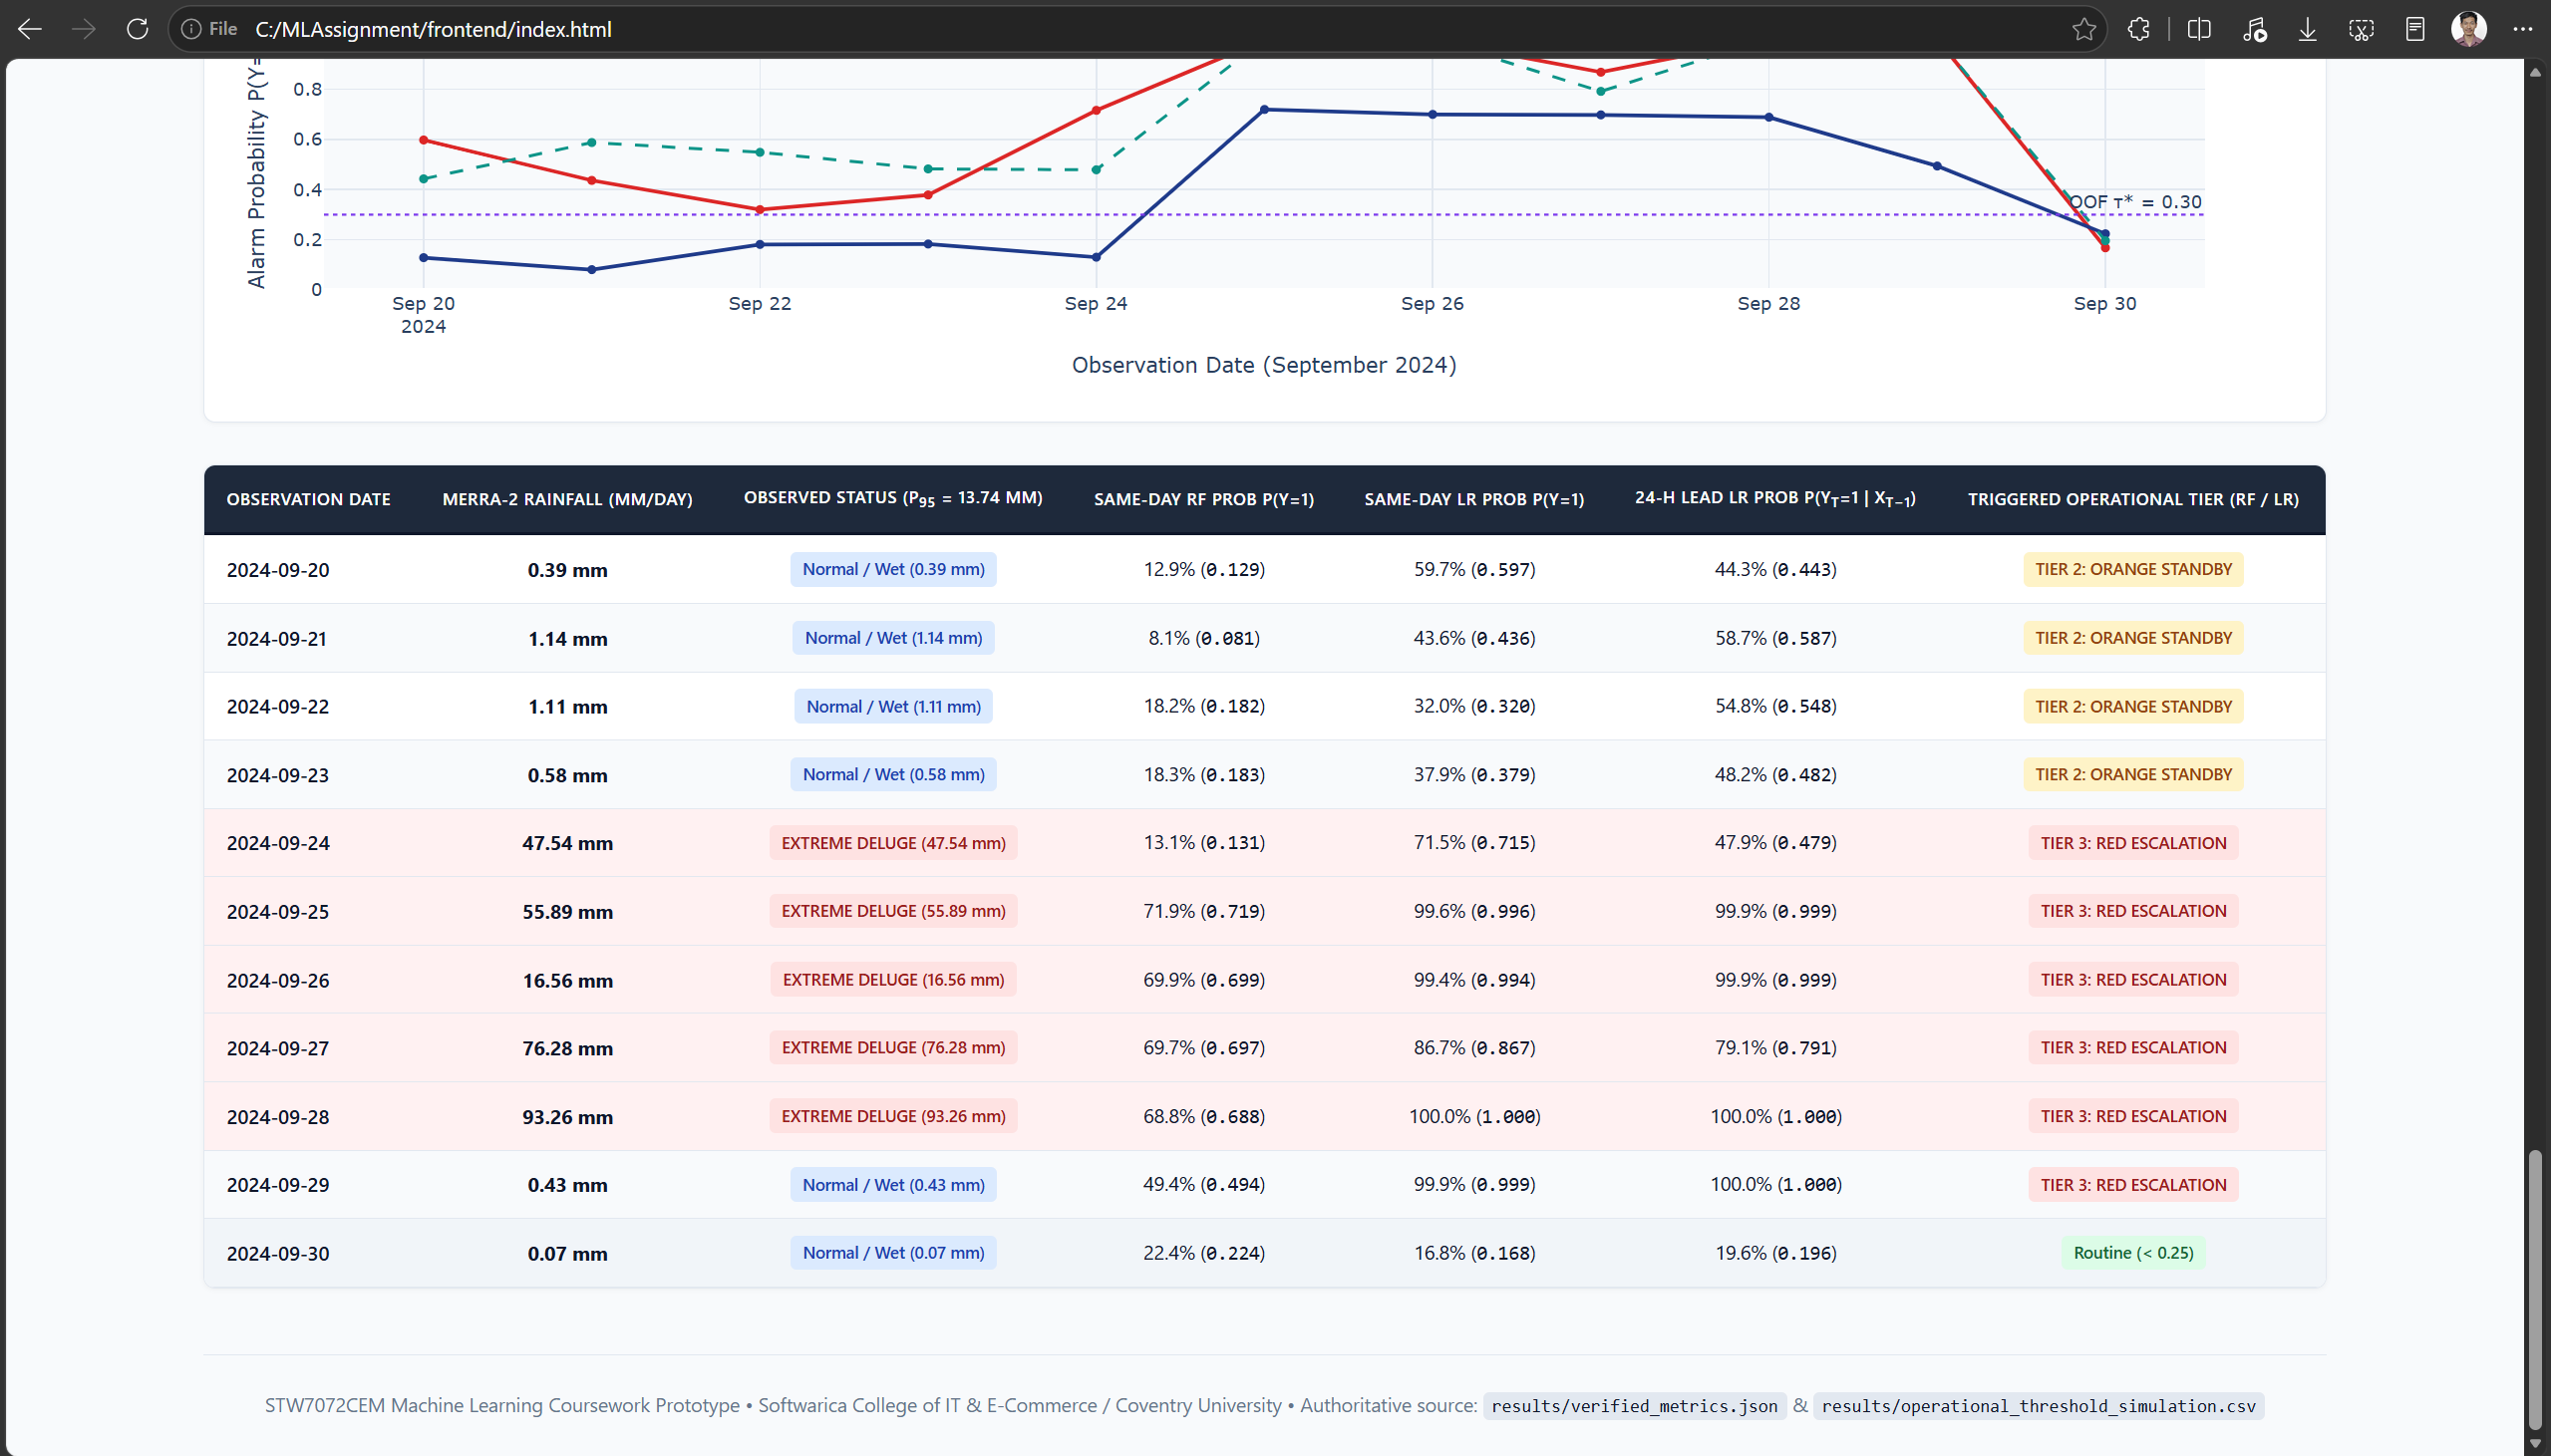
\includegraphics[width=\textwidth,height=0.33\textheight,keepaspectratio]{../figures/dashboard6.png}
\end{minipage}

\end{document}
